% Template for PLoS
% Version 3.5 March 2018
%
% % % % % % % % % % % % % % % % % % % % % %
%
% -- IMPORTANT NOTE
%
% This template contains comments intended
% to minimize problems and delays during our production
% process. Please follow the template instructions
% whenever possible.
%
% % % % % % % % % % % % % % % % % % % % % % %
%
% Once your paper is accepted for publication,
% PLEASE REMOVE ALL TRACKED CHANGES in this file
% and leave only the final text of your manuscript.
% PLOS recommends the use of latexdiff to track changes during review, as this will help to maintain a clean tex file.
% Visit https://www.ctan.org/pkg/latexdiff?lang=en for info or contact us at latex@plos.org.
%
%
% There are no restrictions on package use within the LaTeX files except that
% no packages listed in the template may be deleted.
%
% Please do not include colors or graphics in the text.
%
% The manuscript LaTeX source should be contained within a single file (do not use \input, \externaldocument, or similar commands).
%
% % % % % % % % % % % % % % % % % % % % % % %
%
% -- FIGURES AND TABLES
%
% Please include tables/figure captions directly after the paragraph where they are first cited in the text.
%
% DO NOT INCLUDE GRAPHICS IN YOUR MANUSCRIPT
% - Figures should be uploaded separately from your manuscript file.
% - Figures generated using LaTeX should be extracted and removed from the PDF before submission.
% - Figures containing multiple panels/subfigures must be combined into one image file before submission.
% For figure citations, please use "Fig" instead of "Figure".
% See http://journals.plos.org/plosone/s/figures for PLOS figure guidelines.
%
% Tables should be cell-based and may not contain:
% - spacing/line breaks within cells to alter layout or alignment
% - do not nest tabular environments (no tabular environments within tabular environments)
% - no graphics or colored text (cell background color/shading OK)
% See http://journals.plos.org/plosone/s/tables for table guidelines.
%
% For tables that exceed the width of the text column, use the adjustwidth environment as illustrated in the example table in text below.
%
% % % % % % % % % % % % % % % % % % % % % % % %
%
% -- EQUATIONS, MATH SYMBOLS, SUBSCRIPTS, AND SUPERSCRIPTS
%
% IMPORTANT
% Below are a few tips to help format your equations and other special characters according to our specifications. For more tips to help reduce the possibility of formatting errors during conversion, please see our LaTeX guidelines at http://journals.plos.org/plosone/s/latex
%
% For inline equations, please be sure to include all portions of an equation in the math environment.
%
% Do not include text that is not math in the math environment.
%
% Please add line breaks to long display equations when possible in order to fit size of the column.
%
% For inline equations, please do not include punctuation (commas, etc) within the math environment unless this is part of the equation.
%
% When adding superscript or subscripts outside of brackets/braces, please group using {}.
%
% Do not use \cal for caligraphic font.  Instead, use \mathcal{}
%
% % % % % % % % % % % % % % % % % % % % % % % %
%
% Please contact latex@plos.org with any questions.
%
% % % % % % % % % % % % % % % % % % % % % % % %

\documentclass[10pt,letterpaper]{article}
\usepackage[top=0.85in,left=2.75in,footskip=0.75in]{geometry}

% amsmath and amssymb packages, useful for mathematical formulas and symbols
\usepackage{amsmath,amssymb}

% Use adjustwidth environment to exceed column width (see example table in text)
\usepackage{changepage}

% Use Unicode characters when possible
\usepackage[utf8x]{inputenc}

% textcomp package and marvosym package for additional characters
\usepackage{textcomp,marvosym}

% cite package, to clean up citations in the main text. Do not remove.
% \usepackage{cite}

% Use nameref to cite supporting information files (see Supporting Information section for more info)
\usepackage{nameref,hyperref}

% line numbers
\usepackage[right]{lineno}

% ligatures disabled
\usepackage{microtype}
\DisableLigatures[f]{encoding = *, family = * }

% color can be used to apply background shading to table cells only
\usepackage[table]{xcolor}

% array package and thick rules for tables
\usepackage{array}

% create "+" rule type for thick vertical lines
\newcolumntype{+}{!{\vrule width 2pt}}

% create \thickcline for thick horizontal lines of variable length
\newlength\savedwidth
\newcommand\thickcline[1]{%
  \noalign{\global\savedwidth\arrayrulewidth\global\arrayrulewidth 2pt}%
  \cline{#1}%
  \noalign{\vskip\arrayrulewidth}%
  \noalign{\global\arrayrulewidth\savedwidth}%
}

% \thickhline command for thick horizontal lines that span the table
\newcommand\thickhline{\noalign{\global\savedwidth\arrayrulewidth\global\arrayrulewidth 2pt}%
\hline
\noalign{\global\arrayrulewidth\savedwidth}}


% Remove comment for double spacing
%\usepackage{setspace}
%\doublespacing

% Text layout
\raggedright
\setlength{\parindent}{0.5cm}
\textwidth 5.25in
\textheight 8.75in

% Bold the 'Figure #' in the caption and separate it from the title/caption with a period
% Captions will be left justified
\usepackage[aboveskip=1pt,labelfont=bf,labelsep=period,justification=raggedright,singlelinecheck=off]{caption}
\renewcommand{\figurename}{Fig}

% Use the PLoS provided BiBTeX style
% \bibliographystyle{plos2015}

% Remove brackets from numbering in List of References
\makeatletter
\renewcommand{\@biblabel}[1]{\quad#1.}
\makeatother



% Header and Footer with logo
\usepackage{lastpage,fancyhdr,graphicx}
\usepackage{epstopdf}
%\pagestyle{myheadings}
\pagestyle{fancy}
\fancyhf{}
%\setlength{\headheight}{27.023pt}
%\lhead{\includegraphics[width=2.0in]{PLOS-submission.eps}}
\rfoot{\thepage/\pageref{LastPage}}
\renewcommand{\headrulewidth}{0pt}
\renewcommand{\footrule}{\hrule height 2pt \vspace{2mm}}
\fancyheadoffset[L]{2.25in}
\fancyfootoffset[L]{2.25in}
\lfoot{\today}

%% Include all macros below

\newcommand{\lorem}{{\bf LOREM}}
\newcommand{\ipsum}{{\bf IPSUM}}


% tightlist command for lists without linebreak
\providecommand{\tightlist}{%
  \setlength{\itemsep}{0pt}\setlength{\parskip}{0pt}}


% Pandoc citation processing
\newlength{\cslhangindent}
\setlength{\cslhangindent}{1.5em}
\newlength{\csllabelwidth}
\setlength{\csllabelwidth}{3em}
\newlength{\cslentryspacingunit} % times entry-spacing
\setlength{\cslentryspacingunit}{\parskip}
% for Pandoc 2.8 to 2.10.1
\newenvironment{cslreferences}%
  {}%
  {\par}
% For Pandoc 2.11+
\newenvironment{CSLReferences}[2] % #1 hanging-ident, #2 entry spacing
 {% don't indent paragraphs
  \setlength{\parindent}{0pt}
  % turn on hanging indent if param 1 is 1
  \ifodd #1
  \let\oldpar\par
  \def\par{\hangindent=\cslhangindent\oldpar}
  \fi
  % set entry spacing
  \setlength{\parskip}{#2\cslentryspacingunit}
 }%
 {}
\usepackage{calc}
\newcommand{\CSLBlock}[1]{#1\hfill\break}
\newcommand{\CSLLeftMargin}[1]{\parbox[t]{\csllabelwidth}{#1}}
\newcommand{\CSLRightInline}[1]{\parbox[t]{\linewidth - \csllabelwidth}{#1}\break}
\newcommand{\CSLIndent}[1]{\hspace{\cslhangindent}#1}

\usepackage{lineno}
\usepackage[T1]{fontenc}
\linenumbers
\newcommand{\beginsupplement}{\setcounter{table}{0}  \renewcommand{\thetable}{S\arabic{table}} \setcounter{figure}{0} \renewcommand{\thefigure}{S\arabic{figure}}}
\usepackage{caption}
\usepackage{booktabs}
\usepackage{longtable}
\usepackage{array}
\usepackage{multirow}
\usepackage{wrapfig}
\usepackage{float}
\usepackage{colortbl}
\usepackage{pdflscape}
\usepackage{tabu}
\usepackage{threeparttable}
\usepackage{threeparttablex}
\usepackage[normalem]{ulem}
\usepackage{makecell}
\usepackage{xcolor}


\usepackage{forarray}
\usepackage{xstring}
\newcommand{\getIndex}[2]{
  \ForEach{,}{\IfEq{#1}{\thislevelitem}{\number\thislevelcount\ExitForEach}{}}{#2}
}

\setcounter{secnumdepth}{0}

\newcommand{\getAff}[1]{
  \getIndex{#1}{London School of Hygiene \& Tropical Medicine,Karlsruhe
Institute of Technology Institute of Economic Theory and Statistics,Max
Planck Institute for Multidisciplinary Sciences,UK Health Security
Agency,Imperial College London}
}

\begin{document}
\vspace*{0.2in}

\setcounter{table}{0}  \renewcommand{\thetable}{S\arabic{table}} \setcounter{figure}{0} \renewcommand{\thefigure}{S\arabic{figure}}

\hypertarget{appendix-supplementary-information}{%
\section*{(APPENDIX) Supplementary
information}\label{appendix-supplementary-information}}
\addcontentsline{toc}{section}{(APPENDIX) Supplementary information}

\hypertarget{supplementary-information}{%
\section{Supplementary information}\label{supplementary-information}}

\hypertarget{scoring-metrics-used}{%
\subsection{Scoring metrics used}\label{scoring-metrics-used}}

\begin{longtable}[t]{>{\raggedright\arraybackslash}p{2.5cm}>{\raggedright\arraybackslash}p{9.3cm}}
\caption{\label{tab:scoring-metrics}Overview of the scoring metrics used.}\\
\toprule
Metric & Explanation\\
\midrule
\endfirsthead
\caption[]{Overview of the scoring metrics used. \textit{(continued)}}\\
\toprule
Metric & Explanation\\
\midrule
\endhead

\endfoot
\bottomrule
\endlastfoot
WIS (Weighted) interval score & The weighted interval score (smaller values are better) is a proper scoring rule for quantile forecasts. It converges to the continuos ranked probability score (which itself is a generalisation of the absolute error to probabilistic forecasts) for an increasing number of intervals. The score can be decomposed into a dispersion (uncertainty) component and penalties for over- and underprediction. For a single interval, the score is computed as 
  $$IS_\alpha(F,y) = (u-l) + \frac{2}{\alpha} \cdot (l-y) \cdot 1(y \leq l) + \frac{2}{\alpha} \cdot (y-u) \cdot 1(y \geq u), $$ 
  where $1()$ is the indicator function, $y$ is the true value, and $l$ and $u$ are the $\frac{\alpha}{2}$ and $1 - \frac{\alpha}{2}$ quantiles of the predictive distribution $F$, i.e. the lower and upper bound of a single prediction interval. For a set of $K$ prediction intervals and the median $m$, the score is computed as a weighted sum, 
  $$WIS = \frac{1}{K + 0.5} \cdot \left( w_0 \cdot |y - m| + \sum_{k = 1}^{K} w_k \cdot IS_{\alpha}(F, y) \right), $$
  where $w_k$ is a weight for every interval. Usually, $w_k = \frac{\alpha_k}{2}$ and $w_0 = 0.5$. 

\cellcolor{gray!6}{Its proximity to the absolute error means that when averaging across multiple targets (e.g. different weeks), it will be dominated by targets with higher absolute values.}\\
\addlinespace \addlinespace
Interval coverage & Interval coverage is a measure of marginal calibration and indicates the proportion of observed values that fall in a given prediction interval range. Nominal coverage represents the percentage of observed values that should ideally be covered (e.g. we would like a 50 percent prediction interval to cover on average 50 percent of the observations), while empirical coverage is the actual percentage of observations covered by a certain prediction interval.\\
\addlinespace \addlinespace
Bias & (Relative) bias is a measure of the general tendency of a forecaster to over- or underpredict. Values are between -1 and 1 and 0 ideally. For continuous forecasts, bias is given as 
$$B(F, y) = 1 - 2 \cdot (F (y)), $$ 
where $F$ is the CDF of the predictive distribution and $y$ is the observed value. 

For quantile forecasts, $F(y)$ is replaced by a quantile rank. The appropriate quantile rank is determined by whether the median forecast is below  or above the true value. We then take the innermost quantile rank for which the quantile is still larger (under-prediction) or smaller (over-prediction) than the observed value. 

\cellcolor{gray!6}{In contrast to the over- and underprediction penalties of the interval score it is bound between 0 and 1 and represents a general tendency of forecasts to be biased rather than the absolute amount of over- and underprediction. It is therefore a more robust measurement.}\\*
\end{longtable}

\clearpage

\hypertarget{the-crowdforecasting-app}{%
\subsection{The crowdforecasting app}\label{the-crowdforecasting-app}}

\begin{figure}[H]
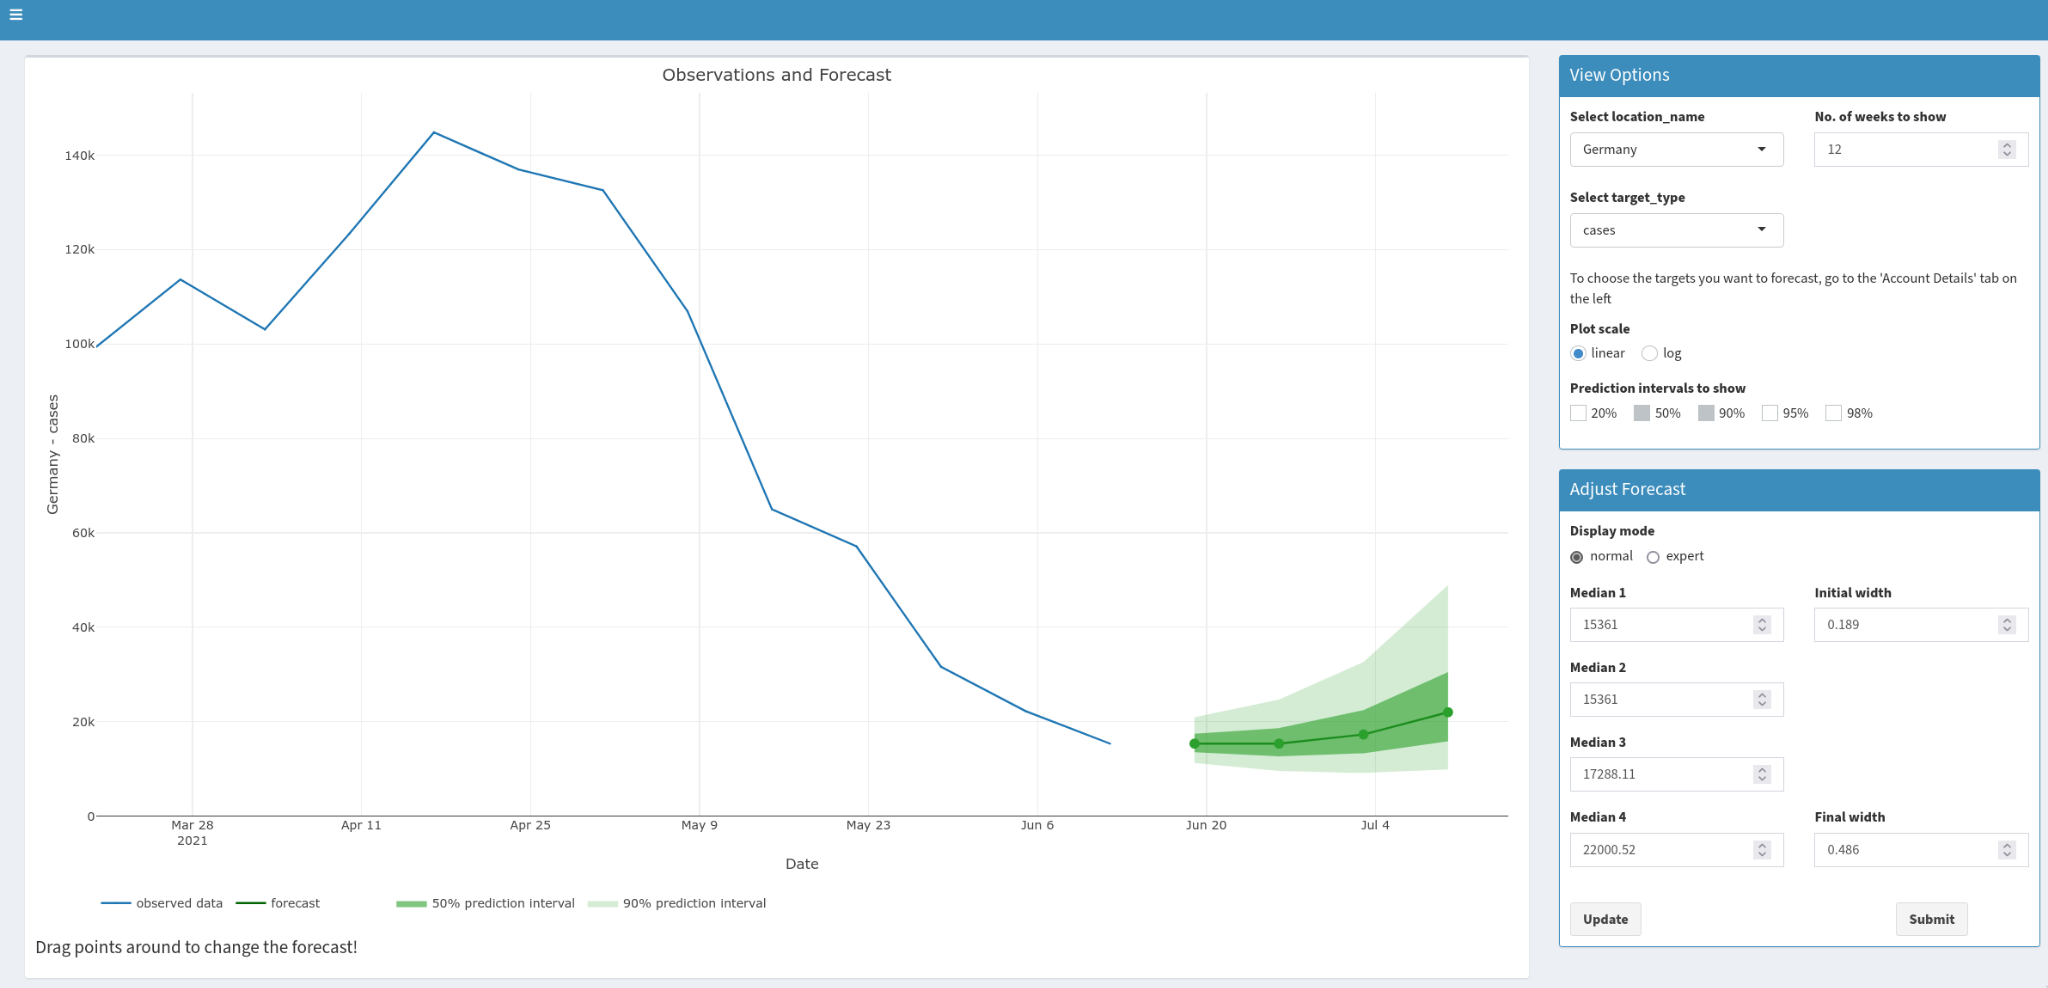
\includegraphics[width=1\linewidth,]{../../../crowd-forecast/Screenshot-forecasting-app} 
\caption{Screenshot of the crowdforecasting app used to elicit predictions (made in June 2021). }\label{fig:screenshot}
\end{figure}

\clearpage

\hypertarget{text-s1.-further-details-on-the-semi-mechanistic-forecasting-models}{%
\subsection{Text S1. Further details on the semi-mechanistic forecasting
models}\label{text-s1.-further-details-on-the-semi-mechanistic-forecasting-models}}

\hypertarget{renewal-equation-model}{%
\subsubsection{Renewal equation model}\label{renewal-equation-model}}

The model was initialised prior to the first observed data point by
assuming constant exponential growth for the mean of assumed delays from
infection to case report.

\begin{align}
  I_{t} &= I_0 \exp  \left(r t \right)  \\
  I_0 &\sim \mathcal{LN}(\log I_{obs}, 0.2) \\
  r &\sim \mathcal{LN}(r_{obs}, 0.2) 
\end{align}

Where \(I_{obs}\) and \(r_{obs}\) are estimated from the first week of
observed data. For the time window of the observed data infections were
then modelled by weighting previous infections by the generation time
and scaling by the instantaneous reproduction number. These infections
were then convolved to cases by date (\(O_t\)) and cases by date of
report (\(D_t\)) using log-normal delay distributions. This model can be
defined mathematically as follows,

\begin{align}
  \log R_{t} &= \log R_{t-1} + \mathrm{GP}_t \\
  I_t &= R_t \sum_{\tau = 1}^{15} w(\tau | \mu_{w}, \sigma_{w}) I_{t - \tau} \\
  O_t &= \sum_{\tau = 0}^{15} \xi_{O}(\tau | \mu_{\xi_{O}}, \sigma_{\xi_{O}}) I_{t-\tau} \\
  D_t &= \alpha \sum_{\tau = 0}^{15} \xi_{D}(\tau | \mu_{\xi_{D}}, \sigma_{\xi_{D}}) O_{t-\tau} \\ 
  C_t &\sim \mathrm{NB}\left(\omega_{(t \mod 7)}D_t, \phi\right)
\end{align}

Where, \begin{align}
     w &\sim \mathcal{G}(\mu_{w}, \sigma_{w}) \\
    \xi_{O} &\sim \mathcal{LN}(\mu_{\xi_{O}}, \sigma_{\xi_{O}}) \\
    \xi_{D} &\sim \mathcal{LN}(\mu_{\xi_{D}}, \sigma_{\xi_{D}}) 
\end{align}

This model used the following priors for cases,

\begin{align}
     R_0 &\sim \mathcal{LN}(0.079, 0.18) \\
    \mu_w &\sim \mathcal{N}(3.6, 0.7) \\
    \sigma_w &\sim \mathcal{N}(3.1, 0.8) \\
    \mu_{\xi_{O}} &\sim \mathcal{N}(1.62, 0.064) \\
    \sigma_{\xi_{O}} &\sim \mathcal{N}(0.418, 0.069) \\
    \mu_{\xi_{D}} &\sim \mathcal{N}(0.614, 0.066) \\
    \sigma_{\xi_{D}} &\sim \mathcal{N}(1.51, 0.048) \\
    \alpha &\sim \mathcal{N}(0.25, 0.05) \\
    \frac{\omega}{7} &\sim \mathrm{Dirichlet}(1, 1, 1, 1, 1, 1, 1) \\
    \phi &\sim \frac{1}{\sqrt{\mathcal{N}(0, 1)}}
\end{align}

and updated the reporting process as follows when forecasting deaths,

\begin{align}
    \mu_{\xi_{D}} &\sim \mathcal{N}(2.29, 0.076) \\
    \sigma_{\xi_{D}} &\sim \mathcal{N}(0.76, 0.055) \\
    \alpha &\sim \mathcal{N}(0.005, 0.0025) 
\end{align}

\(\alpha\), \(\mu\), \(\sigma\), and \(\phi\) were truncated to be
greater than 0 and with \(\xi\), and \(w\) normalised to sum to 1.

The prior for the generation time was sourced from {[}51{]} but refit
using a log-normal incubation period with a mean of 5.2 days (SD 1.1)
and SD of 1.52 days (SD 1.1) with this incubation period also being used
as a prior {[}52{]} for \(\xi_{O}\). This resulted in a
gamma-distributed generation time with mean 3.6 days (standard deviation
(SD) 0.7), and SD of 3.1 days (SD 0.8) for all estimates. We estimated
the delay between symptom onset and case report or death required to
convolve latent infections to observations by fitting an integer
adjusted log-normal distribution to 10 subsampled bootstraps of a public
linelist for cases in Germany from April 2020 to June 2020 with each
bootstrap using 1\% or 1769 samples of the available data {[}45,53{]}
and combining the posteriors for the mean and standard deviation of the
log-normal distribution {[}40,42,46,54{]}.

\(GP_t\) is an approximate Hilbert space Gaussian process as defined in
{[}55{]} using a Matern 3/2 kernel using a boundary factor of 1.5 and 17
basis functions (20\% of the number of days used in fitting). The length
scale of the Gaussian process was given a log-normal prior with a mean
of 21 days, and a standard deviation of 7 days truncated to be greater
than 3 days and less than 60 days. The magnitude of the Gaussian process
was assumed to be normally distributed centred at 0 with a standard
deviation of 0.1.

From the forecast time horizon (\(T\)) and onwards the last value of the
Gaussian process was used (hence \(R_t\) was assumed to be fixed) and
latent infections were adjusted to account for the proportion of the
population that was susceptible to infection as follows,

\begin{equation}
    I_t = (N - I^c_{t-1}) \left(1 - \exp \left(\frac{-I'_t}{N - I^c_{T}}\right)\right),
\end{equation}

where \(I^c_t = \sum_{s< t} I_s\) are cumulative infections by \(t-1\)
and \(I'_t\) are the unadjusted infections defined above. This
adjustment is based on that implemented in the \texttt{epidemia} R
package {[}56,57{]}.

\hypertarget{convolution-model}{%
\paragraph{Convolution model}\label{convolution-model}}

The convolution model shares the same observation model as the renewal
model but rather than assuming that an observation is predicted by
itself using the renewal equation instead assumes that it is predicted
entirely by another observation after some parametric delay. It can be
defined mathematically as follows,

\begin{equation} 
    D_{t} \sim \mathrm{NB}\left(\omega_{(t \mod 7)} \alpha \sum_{\tau = 0}^{30} \xi(\tau | \mu, \sigma) C_{t-\tau},  \phi \right)
\end{equation}

with the following priors,

\begin{align}
    \frac{\omega}{7} &\sim \mathrm{Dirichlet}(1, 1, 1, 1, 1, 1, 1) \\
    \alpha &\sim \mathcal{N}(0.01, 0.02) \\
    \xi &\sim \mathcal{LN}(\mu, \sigma) \\
    \mu &\sim \mathcal{N}(2.5, 0.5) \\
\sigma &\sim \mathcal{N}(0.47, 0.2) \\
\phi &\sim \frac{1}{\sqrt{\mathcal{N}(0, 1)}}
\end{align}

with \(\alpha\), \(\mu\), \(\sigma\), and \(\phi\) truncated to be
greater than 0 and with \(\xi\) normalised such that
\(\sum_{\tau = 0}^{30} \xi(\tau | \mu, \sigma) = 1\).

\hypertarget{model-fitting}{%
\subsubsection{Model fitting}\label{model-fitting}}

Both models were implemented using the \texttt{EpiNow2} R package
(version 1.3.3) {[}40{]}. Each forecast target was fitted independently
for each model using Markov-chain Monte Carlo (MCMC) in stan {[}46{]}. A
minimum of 4 chains were used with a warmup of 250 samples for the
renewal equation-based model and 1000 samples for the convolution model.
2000 samples total post warmup were used for the renewal equation model
and 4000 samples for the convolution model. Different settings were
chosen for each model to optimise compute time contingent on
convergence. Convergence was assessed using the R hat diagnostic
{[}46{]}. For the convolution model forecast the case forecast from the
renewal equation model was used in place of observed cases beyond the
forecast horizon using 1000 posterior samples. 12 weeks of data was used
for both models though only 3 weeks of data were included in the
likelihood for the convolution model.

\clearpage

\hypertarget{tables-with-results-of-the-forecast-evaluation}{%
\subsection{Tables with results of the forecast
evaluation}\label{tables-with-results-of-the-forecast-evaluation}}

\begin{table}[!h]
\caption{\label{tab:score-table-2}Scores for one and two week ahead forecasts (cut to three significant digits and rounded). Note that scores for cases (which include the whole period from October 12th 2020 until March 1st 2021) and deaths (which include only forecasts from the 21st of December 2020 on) are computed on different subsets. Numbers in brackets show the metrics relative to the Hub ensemble (i.e. the median ensemble of all other models submitted to the German and Polish Forecast Hub, excluding our contributions). WIS is the mean weighted interval score (lower values are better), WIS - sd is the standard deviation of all scores achieved by a model. Dispersion, over-prediction and under-prediction together sum up to the weighted interval score. Bias (between -1 and 1, 0 is ideal) represents the general average tendency of a model to over- or underpredict. 50\% and 90\%-coverage are the percentage of observed values that fell within the 50\% and 90\% prediction intervals of a model.\\\hspace{\textwidth}}

\centering
\resizebox{\linewidth}{!}{
\begin{tabular}{>{}llccccccccc}
\toprule
  & Model & WIS & WIS - sd & dispersion & Underpred. & Overpred. & Bias & Abs. error & 50\%-Cov. & 90\%-Cov.\\
\midrule
\addlinespace[0.3em]
\multicolumn{11}{l}{\textbf{Cases}}\\
\hline
\cellcolor{white}{} & Crowd forecast & 7010 (0.8) & 7480 (0.64) & 2680 (0.73) & 1700 (1.38) & 2630 (0.68) & -0.01 & 10400 (0.82) & 0.55 & 0.79\\
\cmidrule{2-11}
\cellcolor{white}{} & Hub-ensemble & 8770 (1) & 11700 (1) & 3670 (1) & 1230 (1) & 3870 (1) & -0.04 & 12700 (1) & 0.57 & 0.81\\
\cmidrule{2-11}
\cellcolor{white}{\multirow{-3}{*}{\raggedright\arraybackslash 1 wk ahead}} & Renewal & 8740 (1) & 11800 (1.01) & 2190 (0.6) & 2720 (2.21) & 3830 (0.99) & 0.18 & 12000 (0.94) & 0.48 & 0.71\\
\cmidrule{1-11}
\cellcolor{white}{} & Crowd forecast & 16200 (0.89) & 16600 (0.76) & 3660 (0.6) & 5930 (1.56) & 6600 (0.78) & -0.01 & 23300 (0.87) & 0.36 & 0.55\\
\cmidrule{2-11}
\cellcolor{white}{} & Hub-ensemble & 18300 (1) & 21900 (1) & 6140 (1) & 3800 (1) & 8410 (1) & -0.03 & 26800 (1) & 0.43 & 0.64\\
\cmidrule{2-11}
\cellcolor{white}{\multirow{-3}{*}{\raggedright\arraybackslash 2 wk ahead}} & Renewal & 25600 (1.4) & 33800 (1.54) & 5420 (0.88) & 5920 (1.56) & 14200 (1.69) & 0.17 & 34600 (1.29) & 0.43 & 0.67\\
\cmidrule{1-11}
\addlinespace[0.3em]
\multicolumn{11}{l}{\textbf{Deaths}}\\
\hline
\cellcolor{white}{} & Convolution & 255 (1.03) & 343 (1.01) & 82 (0.89) & 142 (1.23) & 31.1 (0.75) & -0.18 & 399 (1.19) & 0.42 & 0.79\\
\cmidrule{2-11}
\cellcolor{white}{} & Crowd forecast & 265 (1.07) & 317 (0.94) & 78.2 (0.85) & 82 (0.71) & 105 (2.52) & 0.08 & 402 (1.2) & 0.38 & 0.79\\
\cmidrule{2-11}
\cellcolor{white}{} & Hub-ensemble & 248 (1) & 338 (1) & 92.2 (1) & 115 (1) & 41.6 (1) & -0.04 & 334 (1) & 0.62 & 0.92\\
\cmidrule{2-11}
\cellcolor{white}{\multirow{-4}{*}{\raggedright\arraybackslash 1 wk ahead}} & Renewal & 298 (1.2) & 403 (1.19) & 87 (0.94) & 107 (0.93) & 105 (2.52) & -0.07 & 413 (1.24) & 0.50 & 0.79\\
\cmidrule{1-11}
\cellcolor{white}{} & Convolution & 357 (1.22) & 573 (1.49) & 104 (0.79) & 204 (1.89) & 48.8 (0.94) & -0.10 & 565 (1.32) & 0.33 & 0.79\\
\cmidrule{2-11}
\cellcolor{white}{} & Crowd forecast & 368 (1.26) & 442 (1.15) & 107 (0.81) & 102 (0.94) & 160 (3.08) & 0.14 & 576 (1.34) & 0.38 & 0.75\\
\cmidrule{2-11}
\cellcolor{white}{} & Hub-ensemble & 292 (1) & 385 (1) & 132 (1) & 108 (1) & 51.9 (1) & 0.01 & 429 (1) & 0.62 & 0.96\\
\cmidrule{2-11}
\cellcolor{white}{\multirow{-4}{*}{\raggedright\arraybackslash 2 wk ahead}} & Renewal & 524 (1.79) & 671 (1.74) & 155 (1.17) & 133 (1.23) & 236 (4.55) & -0.02 & 750 (1.75) & 0.50 & 0.71\\
\bottomrule
\end{tabular}}
\end{table}

\begin{table}[!h]
\caption{\label{tab:score-table-4}Scores for three and four week ahead forecasts (cut to three significant digits and rounded). Note that scores for cases (which include the whole period from October 12th 2020 until March 1st 2021) and deaths (which include only forecasts from the 21st of December 2020 on) are computed on different subsets. Numbers in brackets show the metrics relative to the Hub ensemble (i.e. the median ensemble of all other models submitted to the German and Polish Forecast Hub, excluding our contributions). WIS is the mean weighted interval score (lower values are better), WIS - sd is the standard deviation of all scores achieved by a model. Dispersion, over-prediction and under-prediction together sum up to the weighted interval score. Bias (between -1 and 1, 0 is ideal) represents the general average tendency of a model to over- or underpredict. 50\% and 90\%-coverage are the percentage of observed values that fell within the 50\% and 90\% prediction intervals of a model.\\\hspace{\textwidth}}

\centering
\resizebox{\linewidth}{!}{
\begin{tabular}{>{}llccccccccc}
\toprule
  & Model & WIS & WIS - sd & dispersion & Underpred. & Overpred. & Bias & Abs. error & 50\%-Cov. & 90\%-Cov.\\
\midrule
\addlinespace[0.3em]
\multicolumn{11}{l}{\textbf{Cases}}\\
\hline
\cellcolor{white}{} & Crowd forecast & 27000 (0.81) & 26200 (0.64) & 4750 (0.52) & 11000 (1.43) & 11200 (0.67) & 0.02 & 39000 (0.83) & 0.14 & 0.48\\
\cmidrule{2-11}
\cellcolor{white}{} & Hub-ensemble & 33400 (1) & 40700 (1) & 9130 (1) & 7690 (1) & 16600 (1) & -0.01 & 46900 (1) & 0.29 & 0.62\\
\cmidrule{2-11}
\cellcolor{white}{\multirow{-3}{*}{\raggedright\arraybackslash 3 wk ahead}} & Renewal & 50600 (1.51) & 70000 (1.72) & 10800 (1.18) & 7710 (1) & 32100 (1.93) & 0.13 & 68700 (1.46) & 0.29 & 0.55\\
\cmidrule{1-11}
\cellcolor{white}{} & Crowd forecast & 39200 (0.7) & 38600 (0.52) & 5970 (0.49) & 15600 (1.26) & 17600 (0.56) & 0.07 & 54800 (0.74) & 0.05 & 0.38\\
\cmidrule{2-11}
\cellcolor{white}{} & Hub-ensemble & 55900 (1) & 73700 (1) & 12200 (1) & 12400 (1) & 31300 (1) & 0.01 & 74400 (1) & 0.24 & 0.52\\
\cmidrule{2-11}
\cellcolor{white}{\multirow{-3}{*}{\raggedright\arraybackslash 4 wk ahead}} & Renewal & 91700 (1.64) & 135000 (1.83) & 19500 (1.6) & 8990 (0.72) & 63200 (2.02) & 0.09 & 125000 (1.68) & 0.31 & 0.48\\
\cmidrule{1-11}
\addlinespace[0.3em]
\multicolumn{11}{l}{\textbf{Deaths}}\\
\hline
\cellcolor{white}{} & Convolution & 541 (1.7) & 802 (2.45) & 157 (0.91) & 279 (3.01) & 105 (1.91) & -0.04 & 747 (1.53) & 0.54 & 0.75\\
\cmidrule{2-11}
\cellcolor{white}{} & Crowd forecast & 414 (1.3) & 526 (1.6) & 137 (0.8) & 82 (0.88) & 194 (3.52) & 0.12 & 648 (1.33) & 0.42 & 0.83\\
\cmidrule{2-11}
\cellcolor{white}{} & Hub-ensemble & 319 (1) & 328 (1) & 172 (1) & 92.7 (1) & 55.1 (1) & -0.03 & 488 (1) & 0.54 & 0.96\\
\cmidrule{2-11}
\cellcolor{white}{\multirow{-4}{*}{\raggedright\arraybackslash 3 wk ahead}} & Renewal & 724 (2.27) & 916 (2.79) & 249 (1.45) & 158 (1.7) & 317 (5.75) & -0.01 & 1040 (2.13) & 0.46 & 0.83\\
\cmidrule{1-11}
\cellcolor{white}{} & Convolution & 763 (1.8) & 932 (2.1) & 268 (1.26) & 331 (2.63) & 164 (1.91) & 0.01 & 985 (1.46) & 0.54 & 0.75\\
\cmidrule{2-11}
\cellcolor{white}{} & Crowd forecast & 498 (1.17) & 633 (1.43) & 168 (0.79) & 83.6 (0.66) & 246 (2.87) & 0.14 & 756 (1.12) & 0.38 & 0.79\\
\cmidrule{2-11}
\cellcolor{white}{} & Hub-ensemble & 424 (1) & 443 (1) & 212 (1) & 126 (1) & 85.7 (1) & -0.06 & 675 (1) & 0.58 & 0.92\\
\cmidrule{2-11}
\cellcolor{white}{\multirow{-4}{*}{\raggedright\arraybackslash 4 wk ahead}} & Renewal & 959 (2.26) & 1210 (2.73) & 337 (1.59) & 200 (1.59) & 421 (4.91) & -0.05 & 1350 (2) & 0.50 & 0.79\\
\bottomrule
\end{tabular}}
\end{table}

\clearpage

\hypertarget{aggregate-performance-by-location}{%
\subsection{Aggregate performance by
location}\label{aggregate-performance-by-location}}

\hypertarget{performance-in-germany}{%
\subsubsection{Performance in Germany}\label{performance-in-germany}}

\begin{figure}[H]
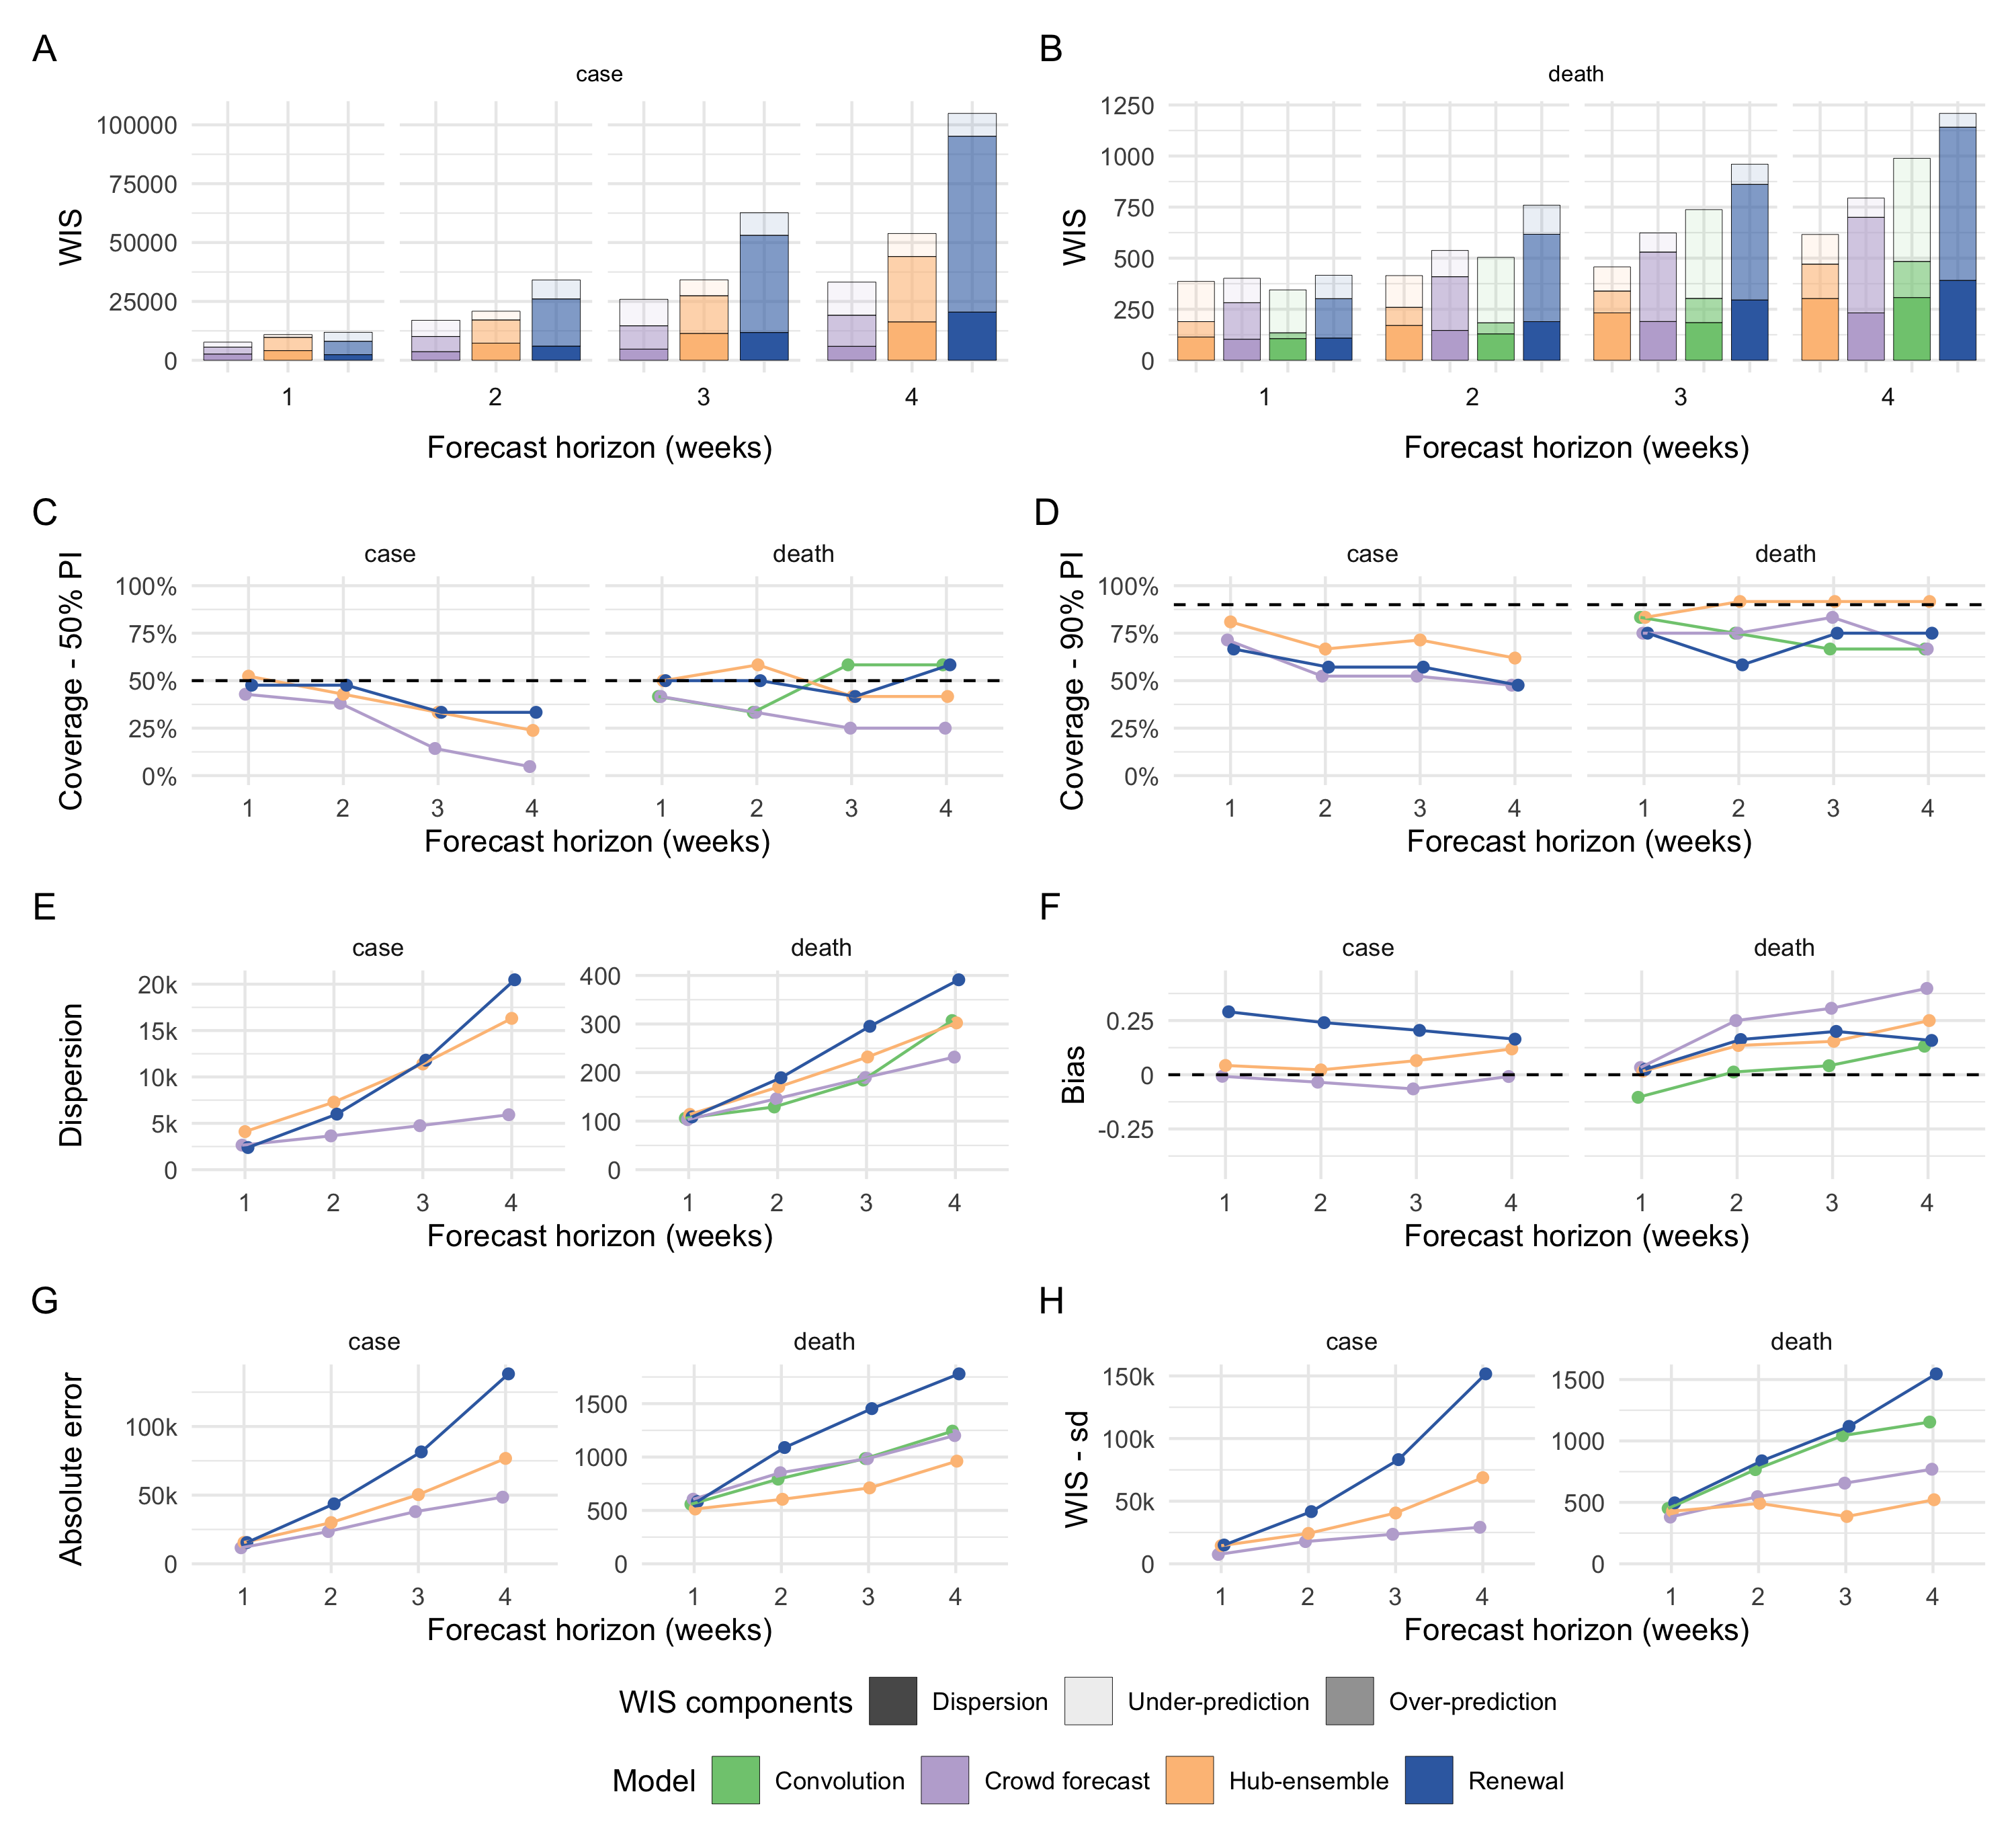
\includegraphics[width=1\linewidth,]{../../../analysis/plots/aggregate-performance-all-Germany-v4}
\caption{Visualisation of aggregate performance metrics for forecasts one to four weeks into the future in Germany. A, B: mean weighted interval score (WIS, lower indicates better performance) across horizons. WIS is decomposed into its components dispersion, over-prediction and under-prediction. C: Empirical coverage of the 50\% prediction intervals (50\% coverage is perfect). D: Empirical coverage of the 90\% prediction intervals. E: Dispersion (same as in panel A, B). Higher values mean greater dispersion of the forecast and imply ceteris paribus a worse score. F: Bias, i.e. general (relative) tendency to over- or underpredict. Values are between -1 (complete under-prediction) and 1 (complete over-prediction) and 0 ideally. G: Absolute error of the median forecast (lower is better). H. Standard deviation of all WIS values for different horizons}\label{fig:agg-performance-all-Germany}
\end{figure}

\hypertarget{performance-in-poland}{%
\subsubsection{Performance in Poland}\label{performance-in-poland}}

\begin{figure}[H]
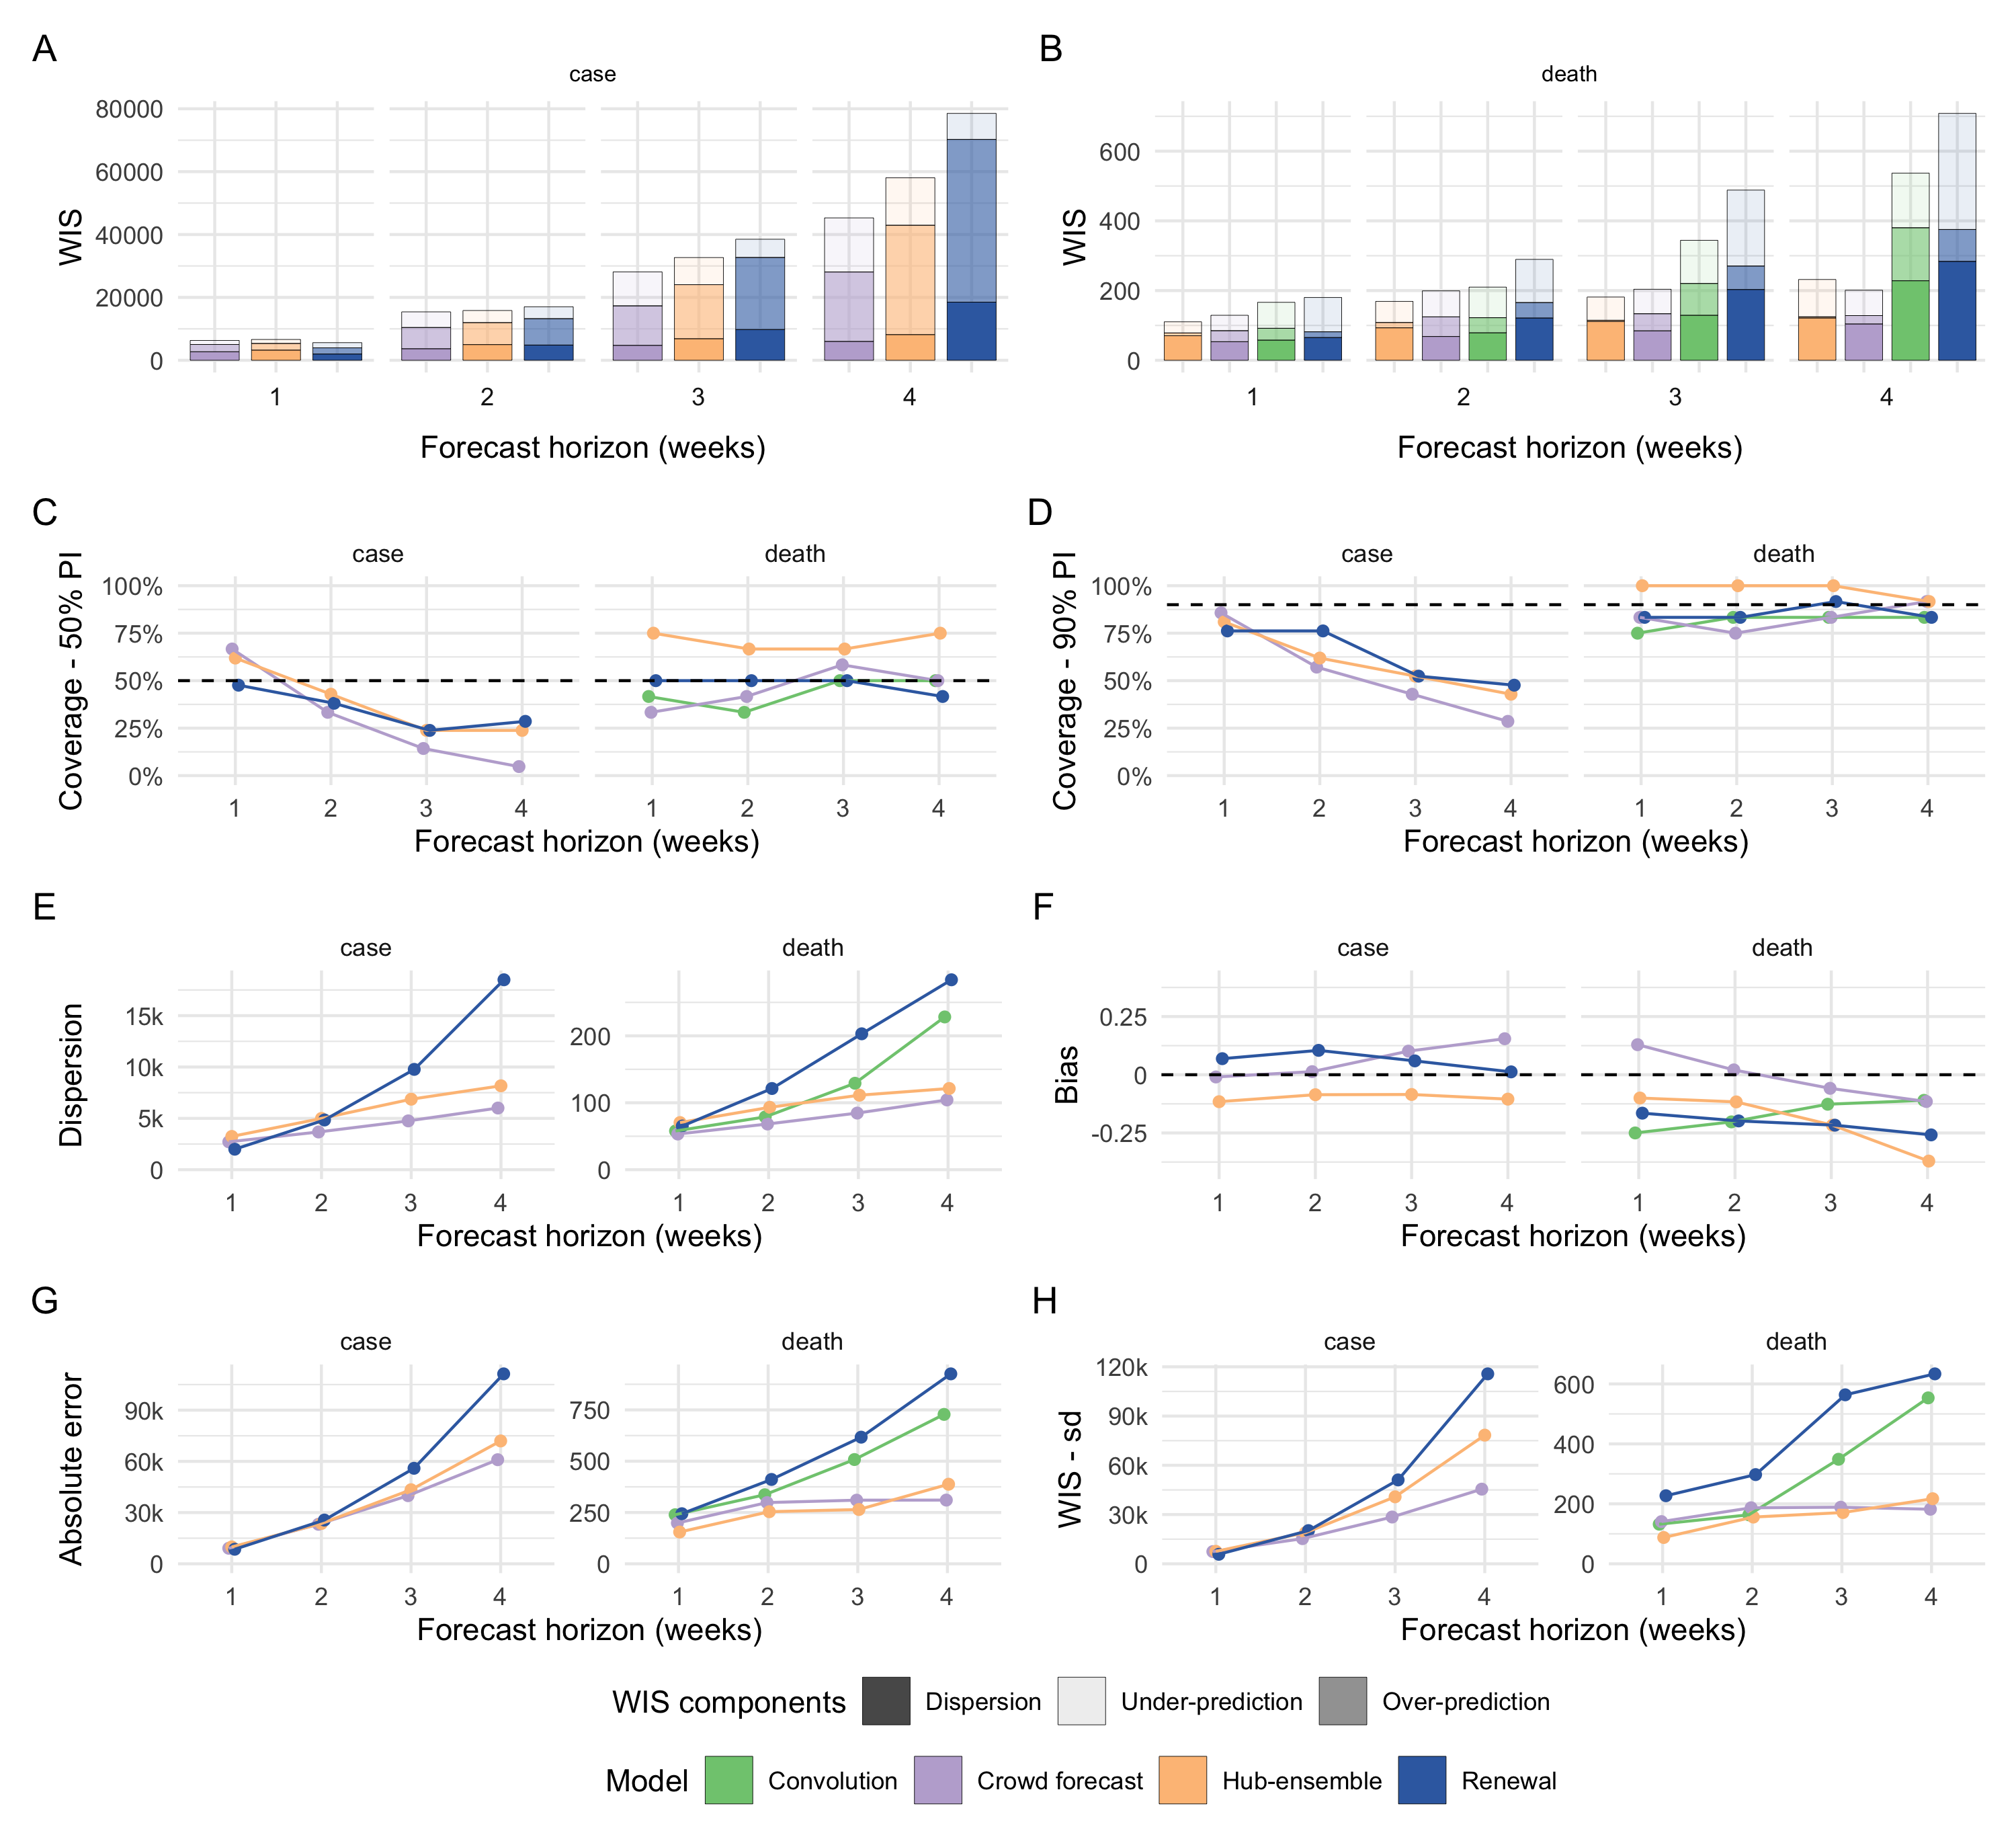
\includegraphics[width=1\linewidth,]{../../../analysis/plots/aggregate-performance-all-Poland-v4}
\caption{Visualisation of aggregate performance metrics for forecasts one to four weeks into the future in Poland. A, B: mean weighted interval score (WIS, lower indicates better performance) across horizons. WIS is decomposed into its components dispersion, over-prediction and under-prediction. C: Empirical coverage of the 50\% prediction intervals (50\% coverage is perfect). D: Empirical coverage of the 90\% prediction intervals. E: Dispersion (same as in panel A, B). Higher values mean greater dispersion of the forecast and imply ceteris paribus a worse score. F: Bias, i.e. general (relative) tendency to over- or underpredict. Values are between -1 (complete under-prediction) and 1 (complete over-prediction) and 0 ideally. G: Absolute error of the median forecast (lower is better). H. Standard deviation of all WIS values for different horizons}\label{fig:agg-performance-all-Poland}
\end{figure}

\hypertarget{performance-across-locations-in-absolute-terms}{%
\subsubsection{Performance across locations in absolute
terms}\label{performance-across-locations-in-absolute-terms}}

\begin{figure}[H]
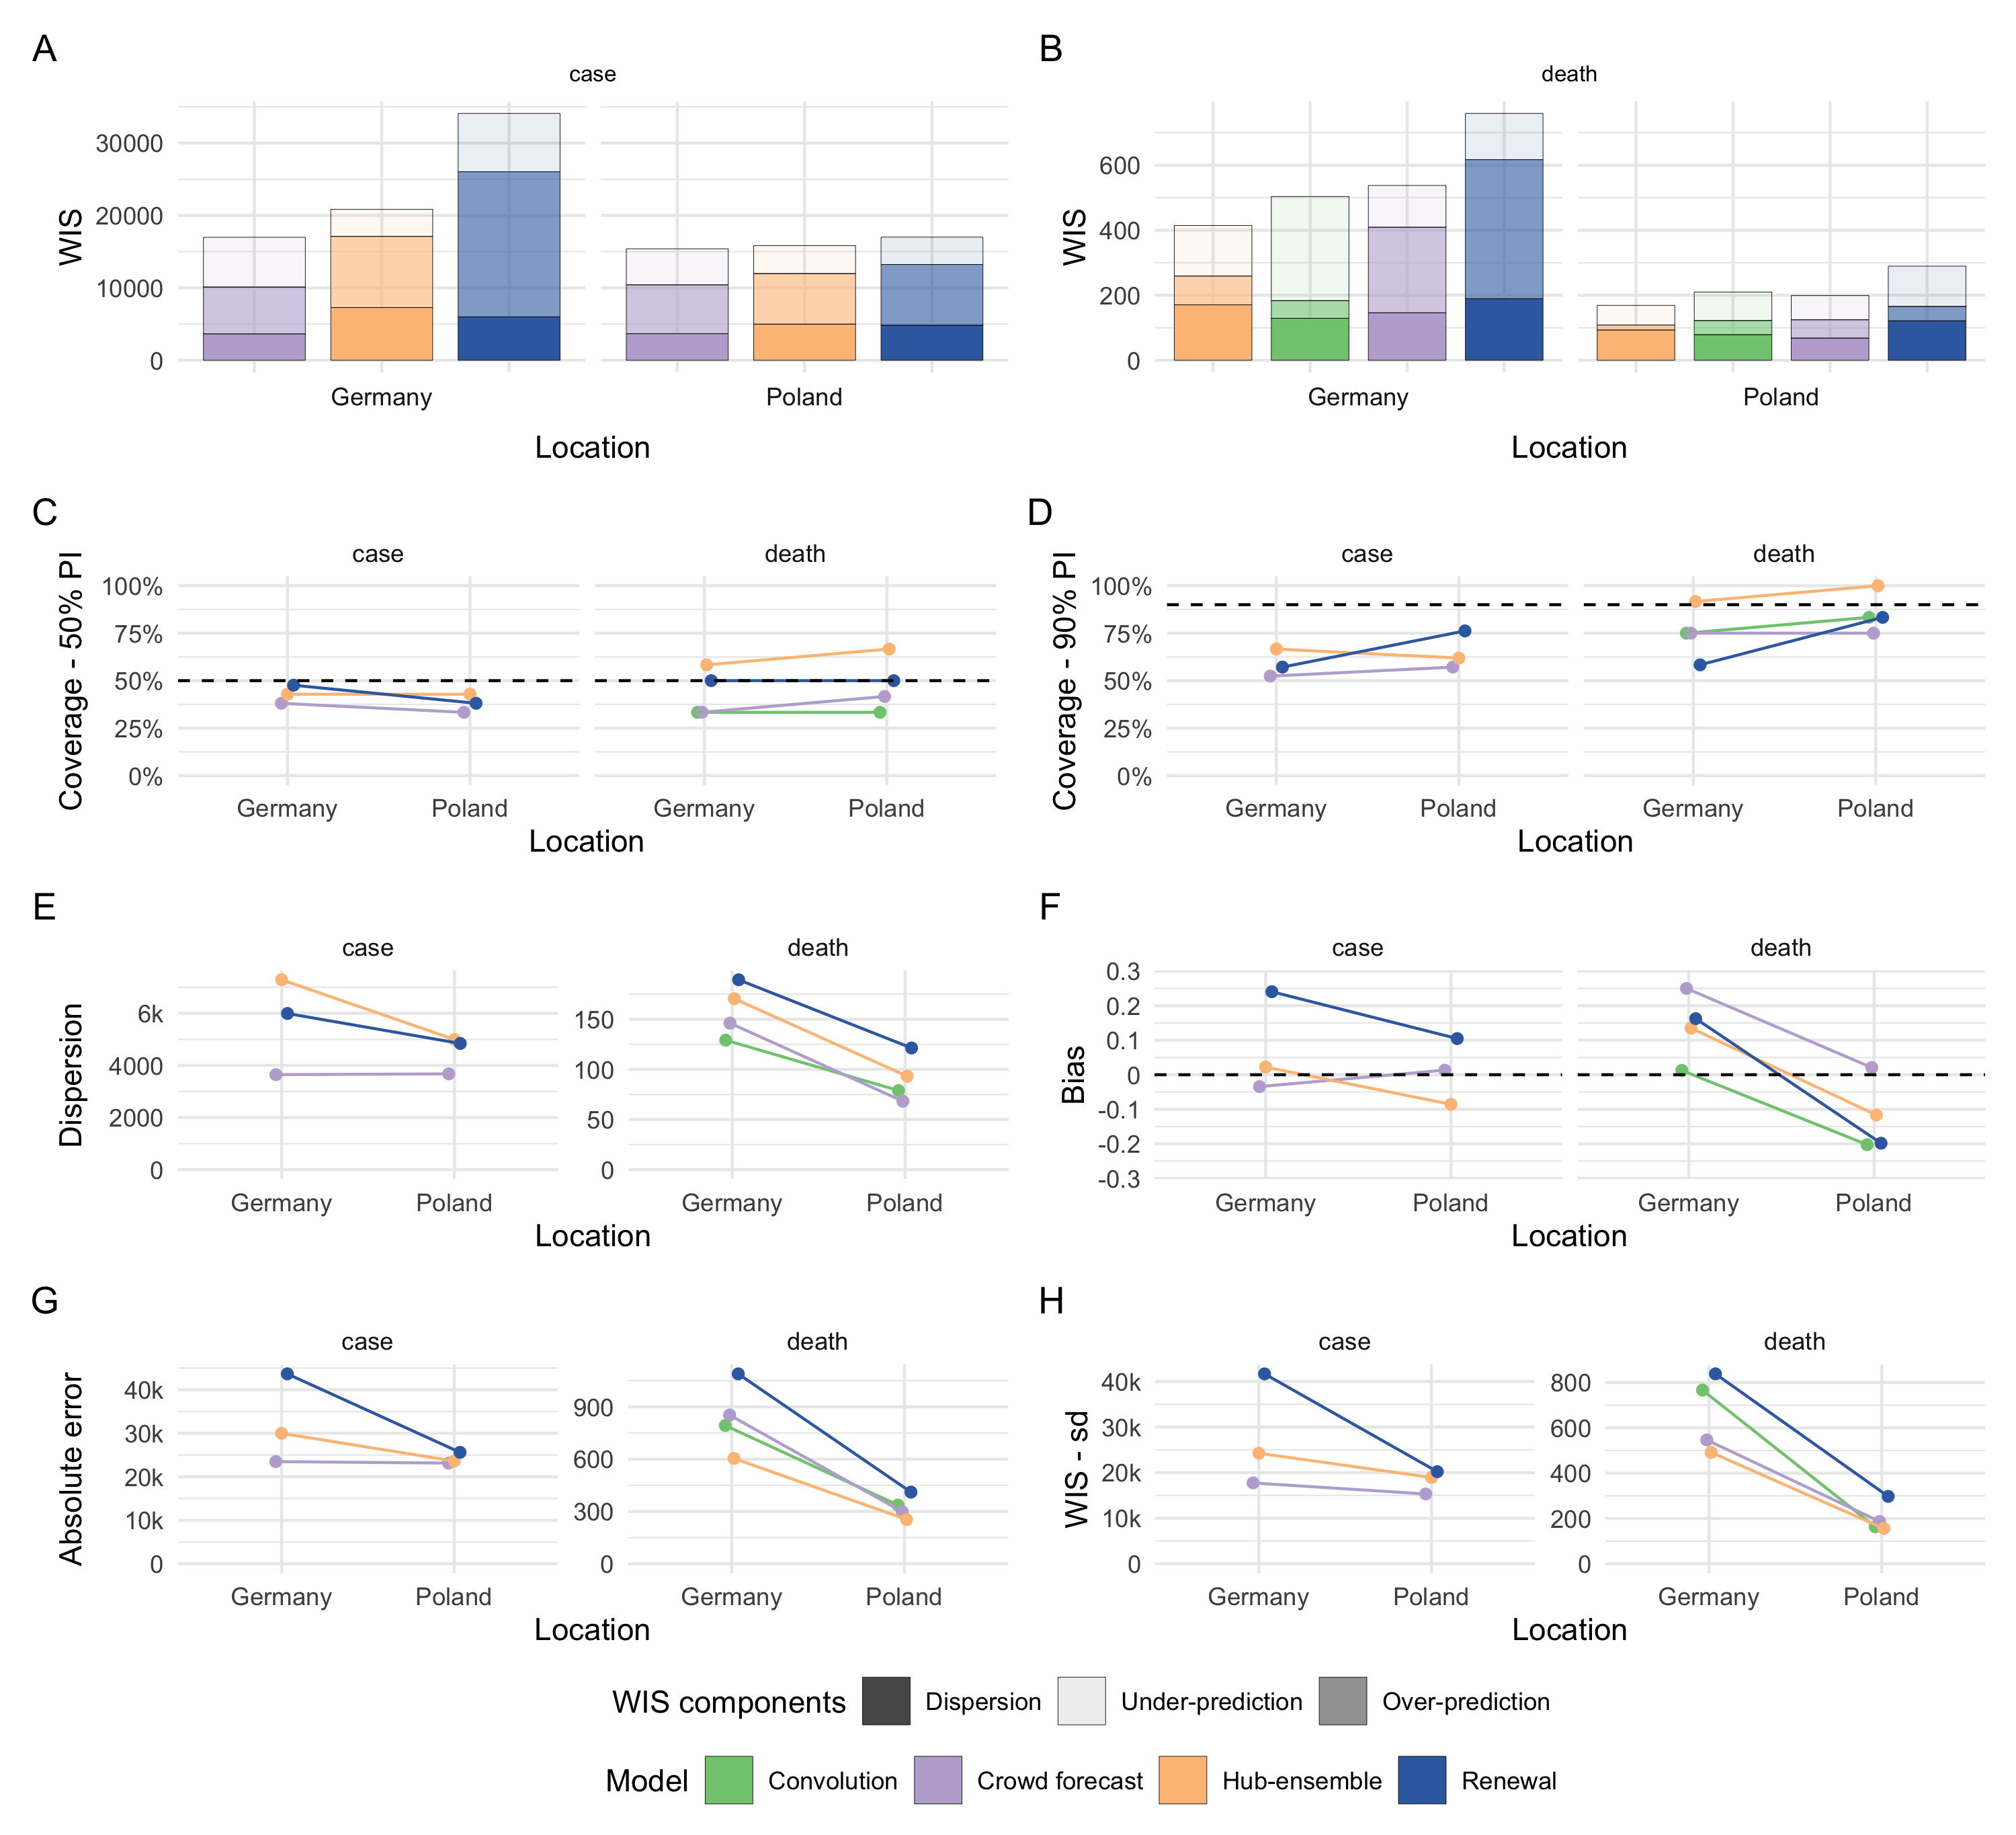
\includegraphics[width=1\linewidth,]{../../../analysis/plots/aggregate-performance-2-weeks-locations-all-v4}
\caption{Visualisation of aggregate performance metrics across locations. A, B: mean weighted interval score (WIS, lower indicates better performance) across horizons. WIS is decomposed into its components dispersion, over-prediction and under-prediction. C: Empirical coverage of the 50\% prediction intervals (50\% coverage is perfect). D: Empirical coverage of the 90\% prediction intervals. E: Dispersion (same as in panel A, B). Higher values mean greater dispersion of the forecast and imply ceteris paribus a worse score. F: Bias, i.e. general (relative) tendency to over- or underpredict. Values are between -1 (complete under-prediction) and 1 (complete over-prediction) and 0 ideally. G: Absolute error of the median forecast (lower is better). H. Standard deviation of WIS values.}\label{fig:performance-locations}
\end{figure}

\hypertarget{performance-across-locations-in-relative-terms}{%
\subsection{Performance across locations in relative
terms}\label{performance-across-locations-in-relative-terms}}

\begin{figure}[H]
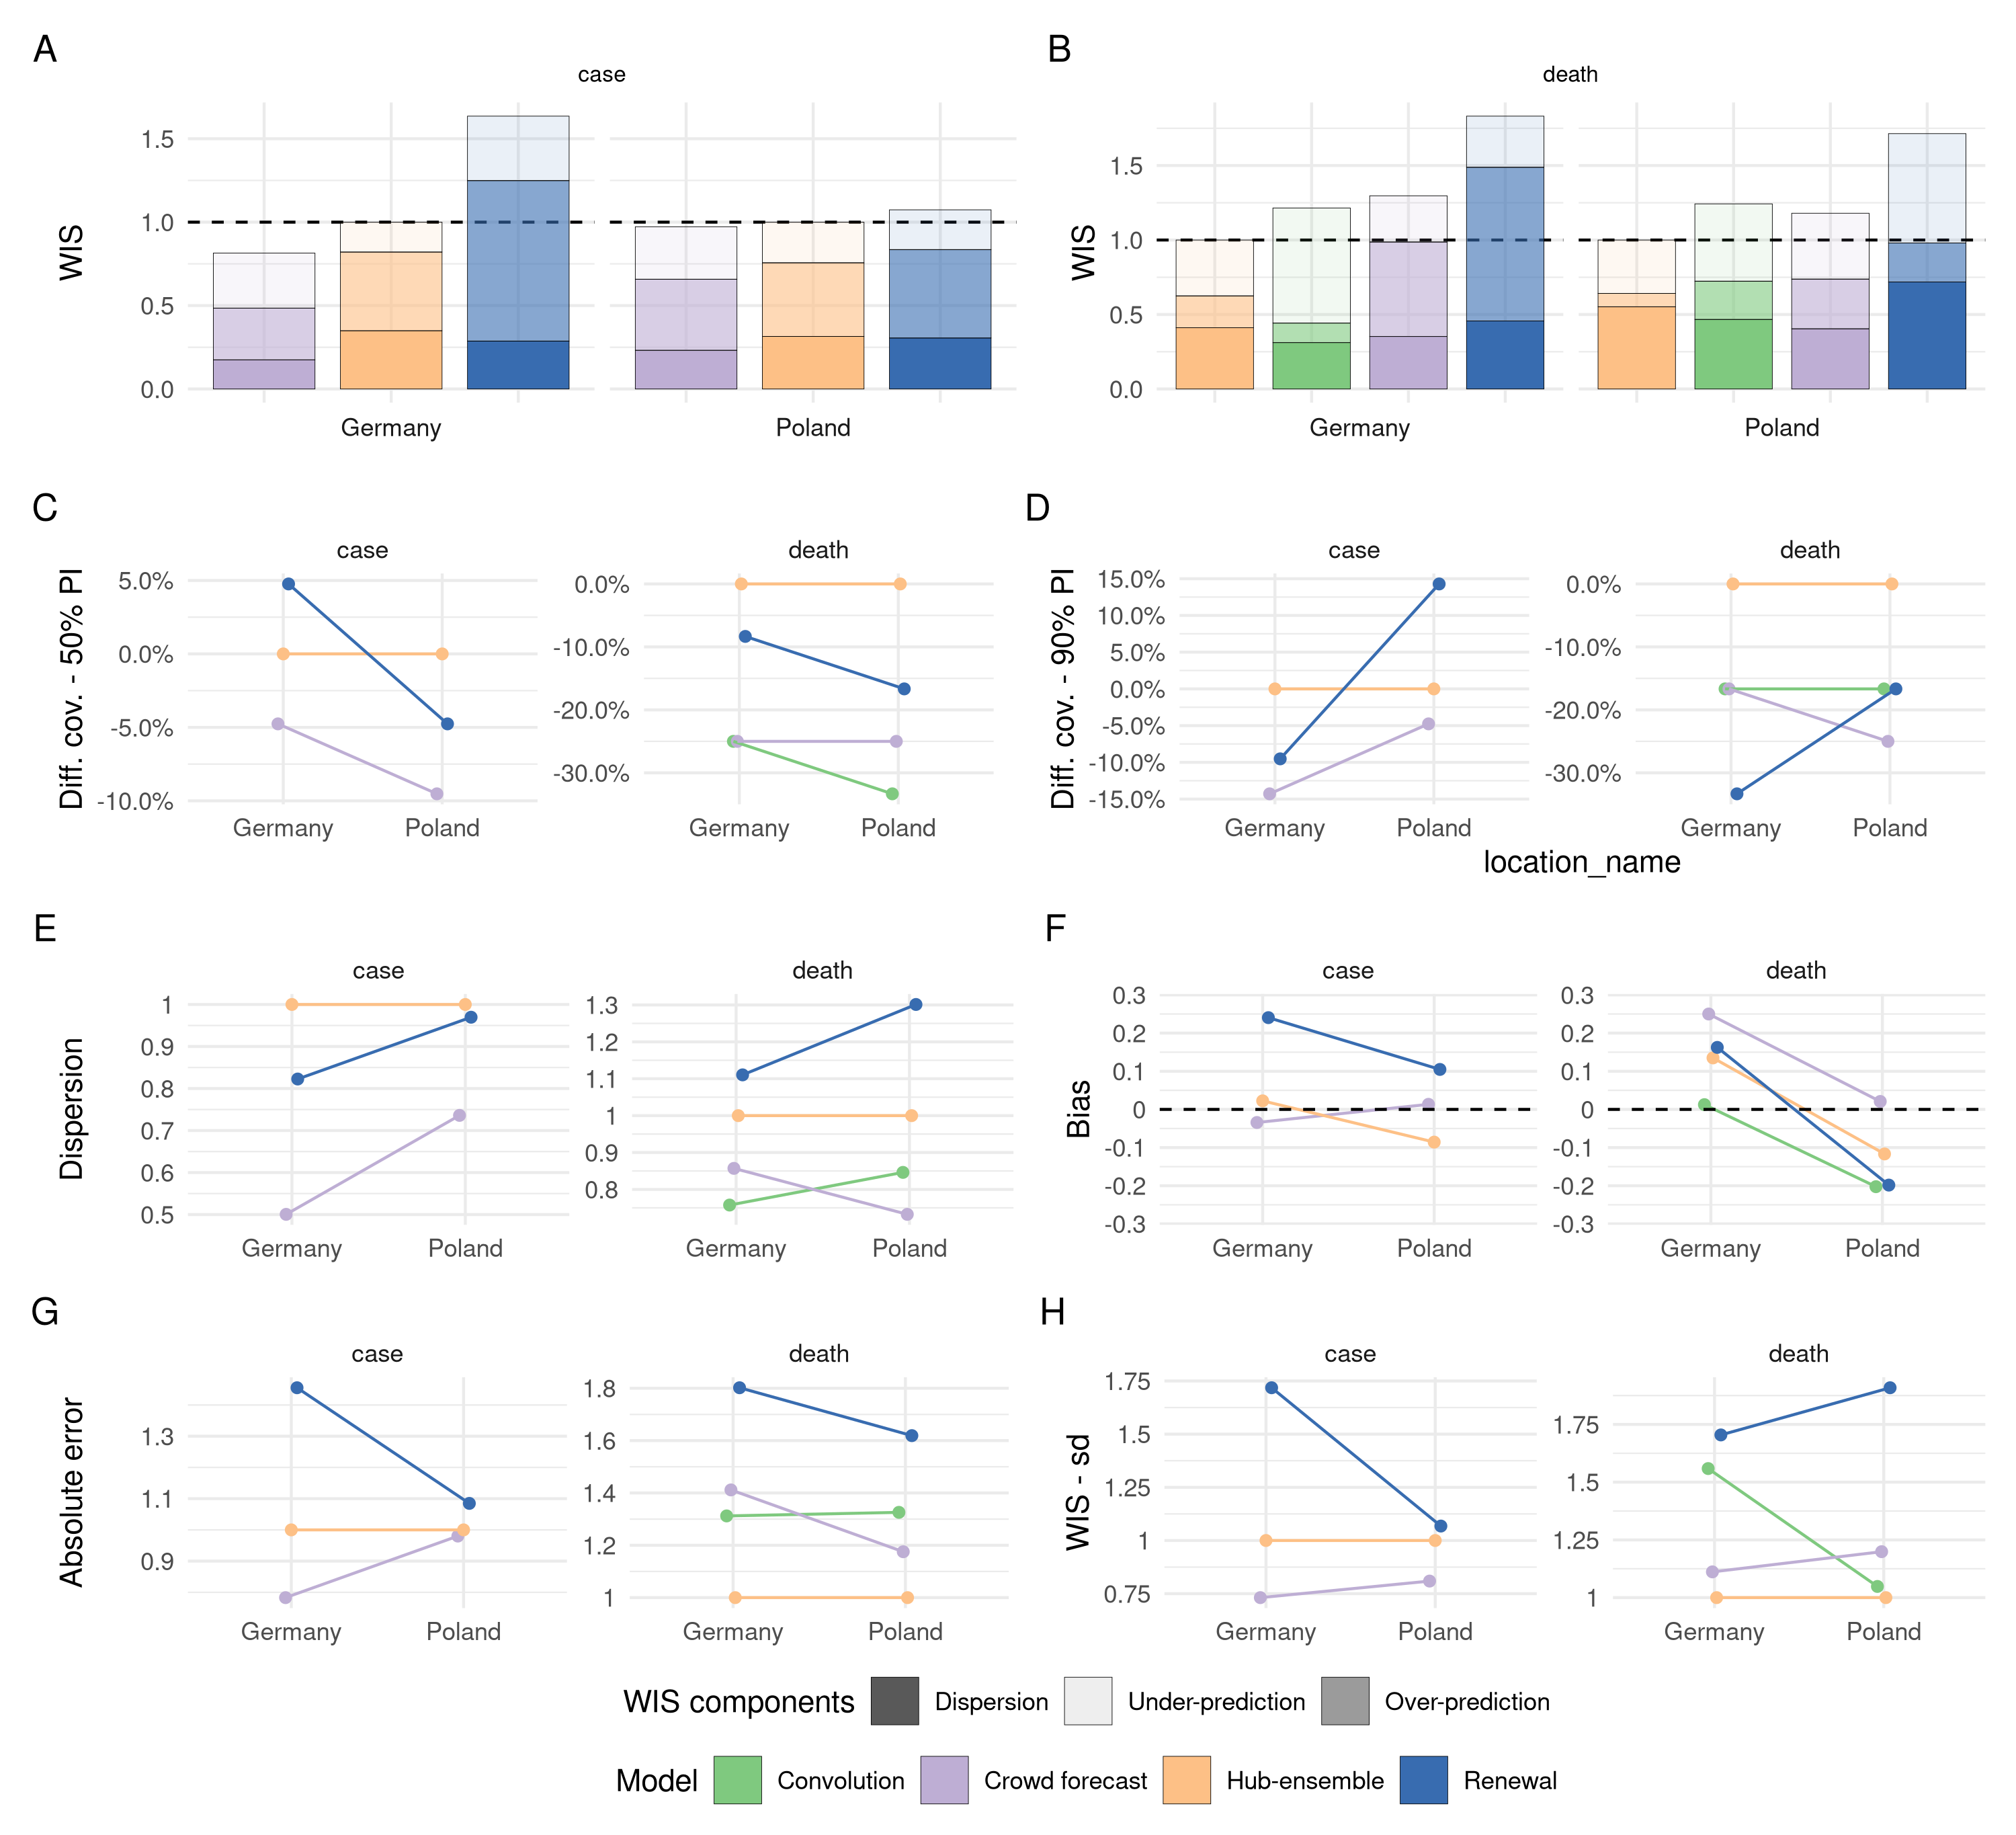
\includegraphics[width=1\linewidth,]{../../../analysis/plots/aggregate-performance-2-weeks-locations-all-rel-v4}
\caption{Visualisation of relative aggregate performance metrics across locations. A, B: mean weighted interval score (WIS) across locations (lower values indicate better performance). C, D: Empirical coverage of the 50\% and 90\% prediction intervals. E: Dispersion. Higher values mean greater dispersion of the forecast and imply ceteris paribus a worse score. F: Bias, i.e. general (relative) tendency to over- orunderpredict. Values are between -1 (complete under-prediction) and 1 (complete over-prediction) and 0 ideally. G: Absolute error of the median forecast. H. Standard deviation of WIS values.}\label{fig:performance-locations-rel}
\end{figure}

\clearpage

\hypertarget{visualisation-of-daily-reported-cases-and-deaths}{%
\subsection{Visualisation of daily reported cases and
deaths}\label{visualisation-of-daily-reported-cases-and-deaths}}

\begin{figure}[H]
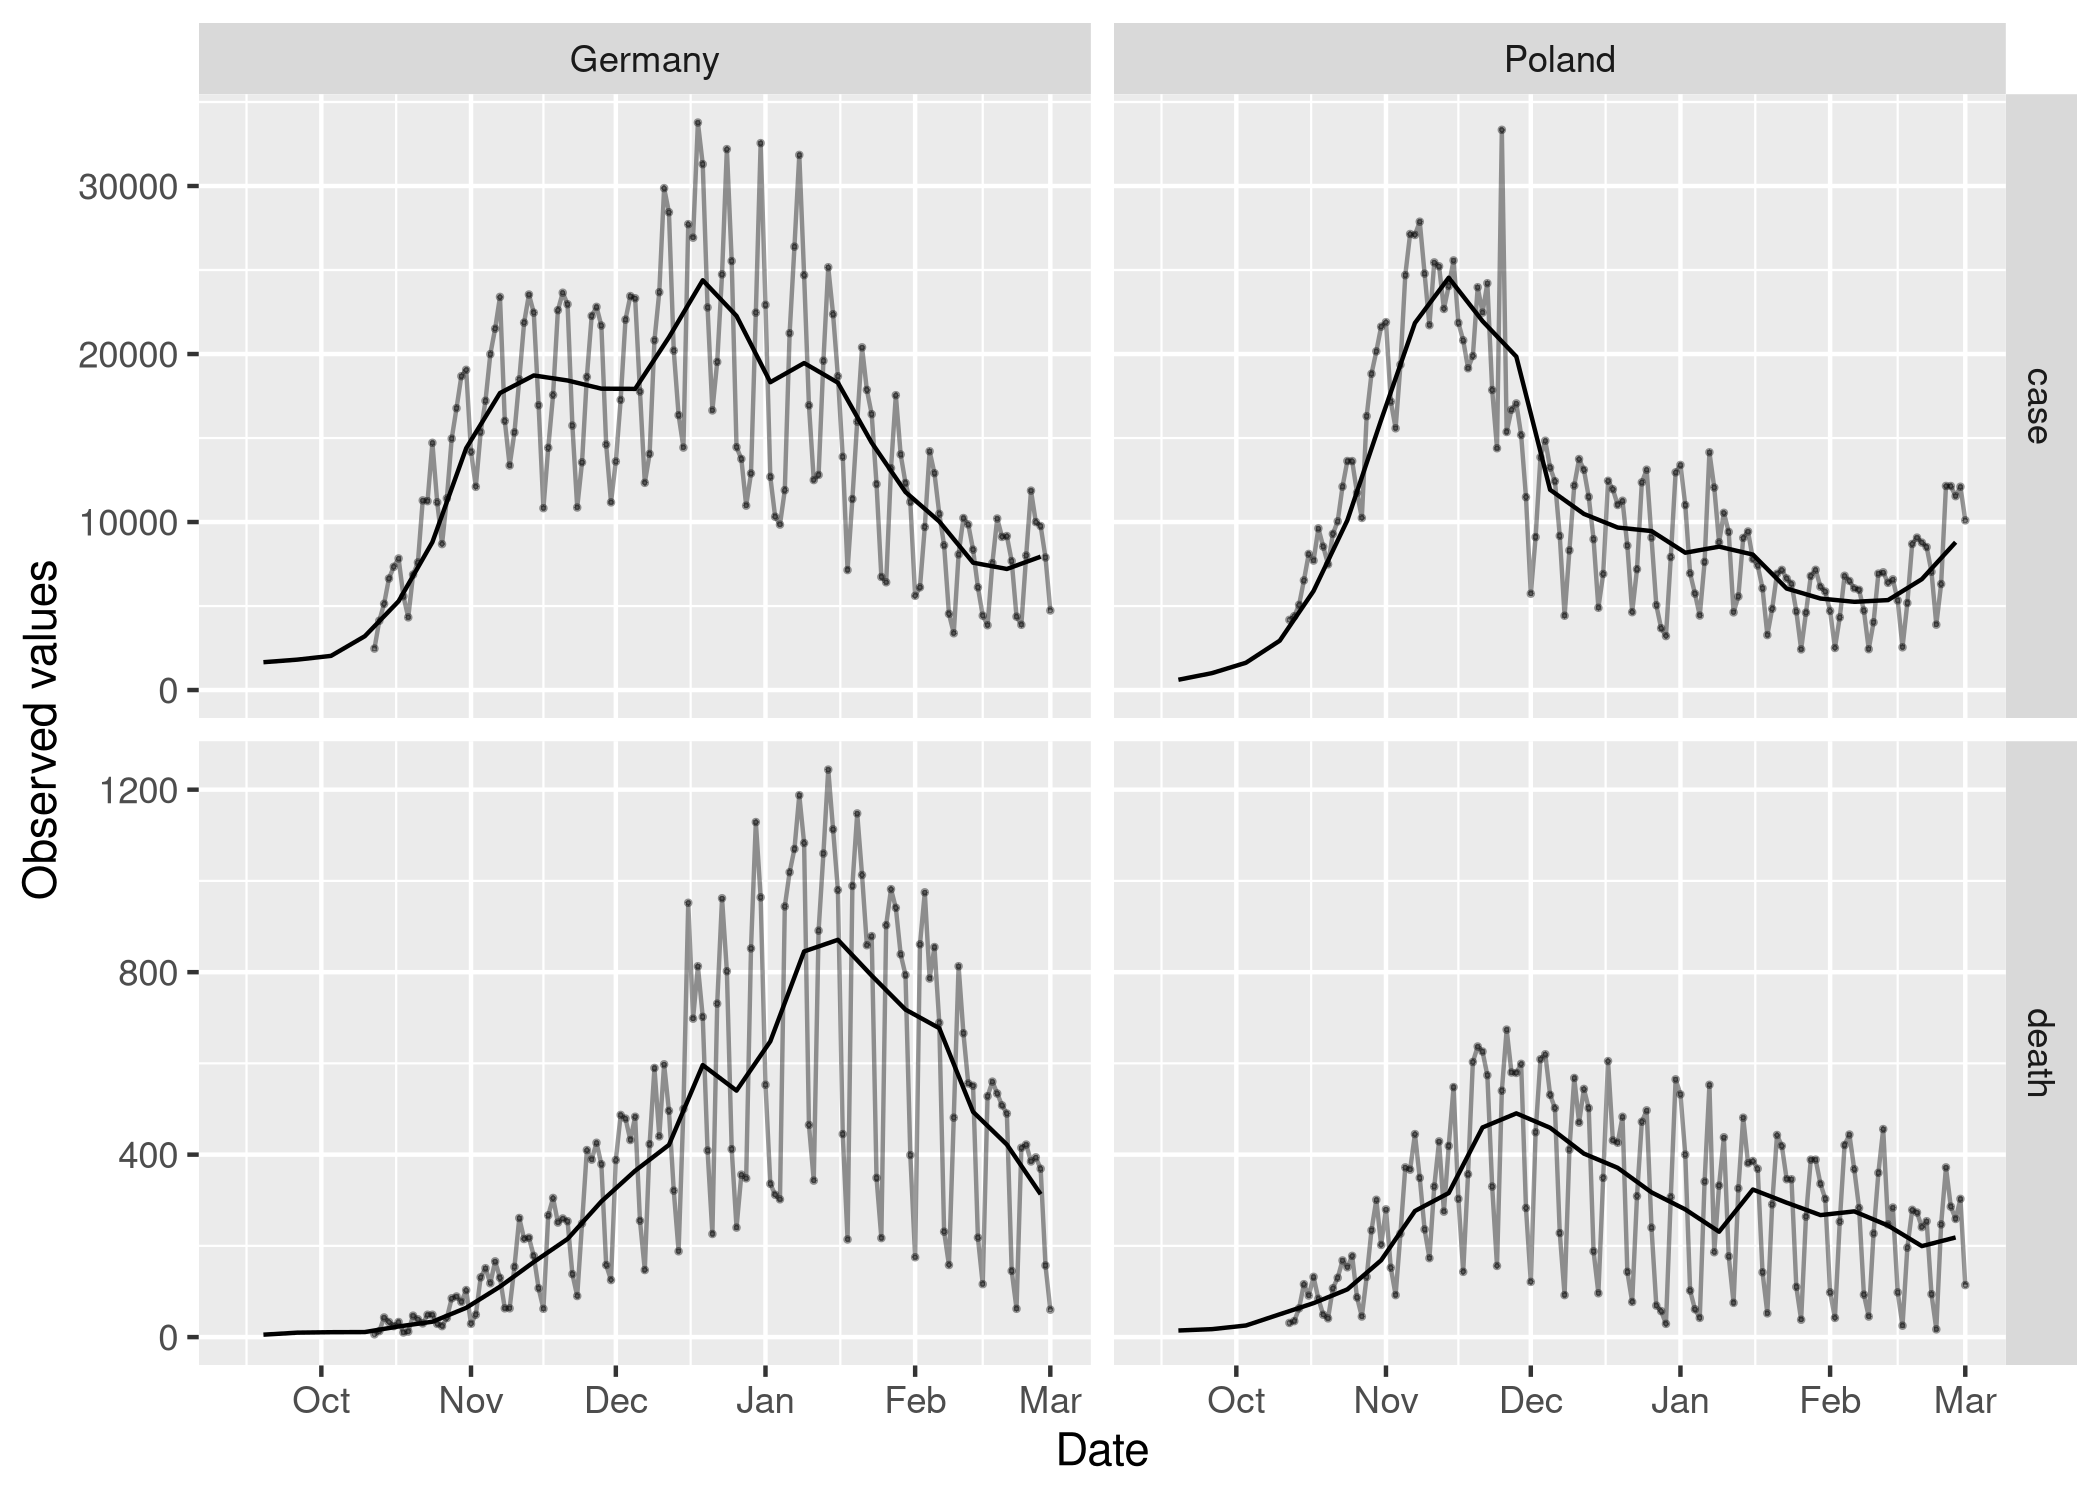
\includegraphics[width=1\linewidth,]{../../../analysis/plots/daily_truth} 
\caption{Visualisation of daily report data. The black line represents weekly data divided by seven. Data were last accessed through the German and Polish Forecast Hub on August 21 2021.}\label{fig:daily-truth}
\end{figure}

\begin{figure}[H]
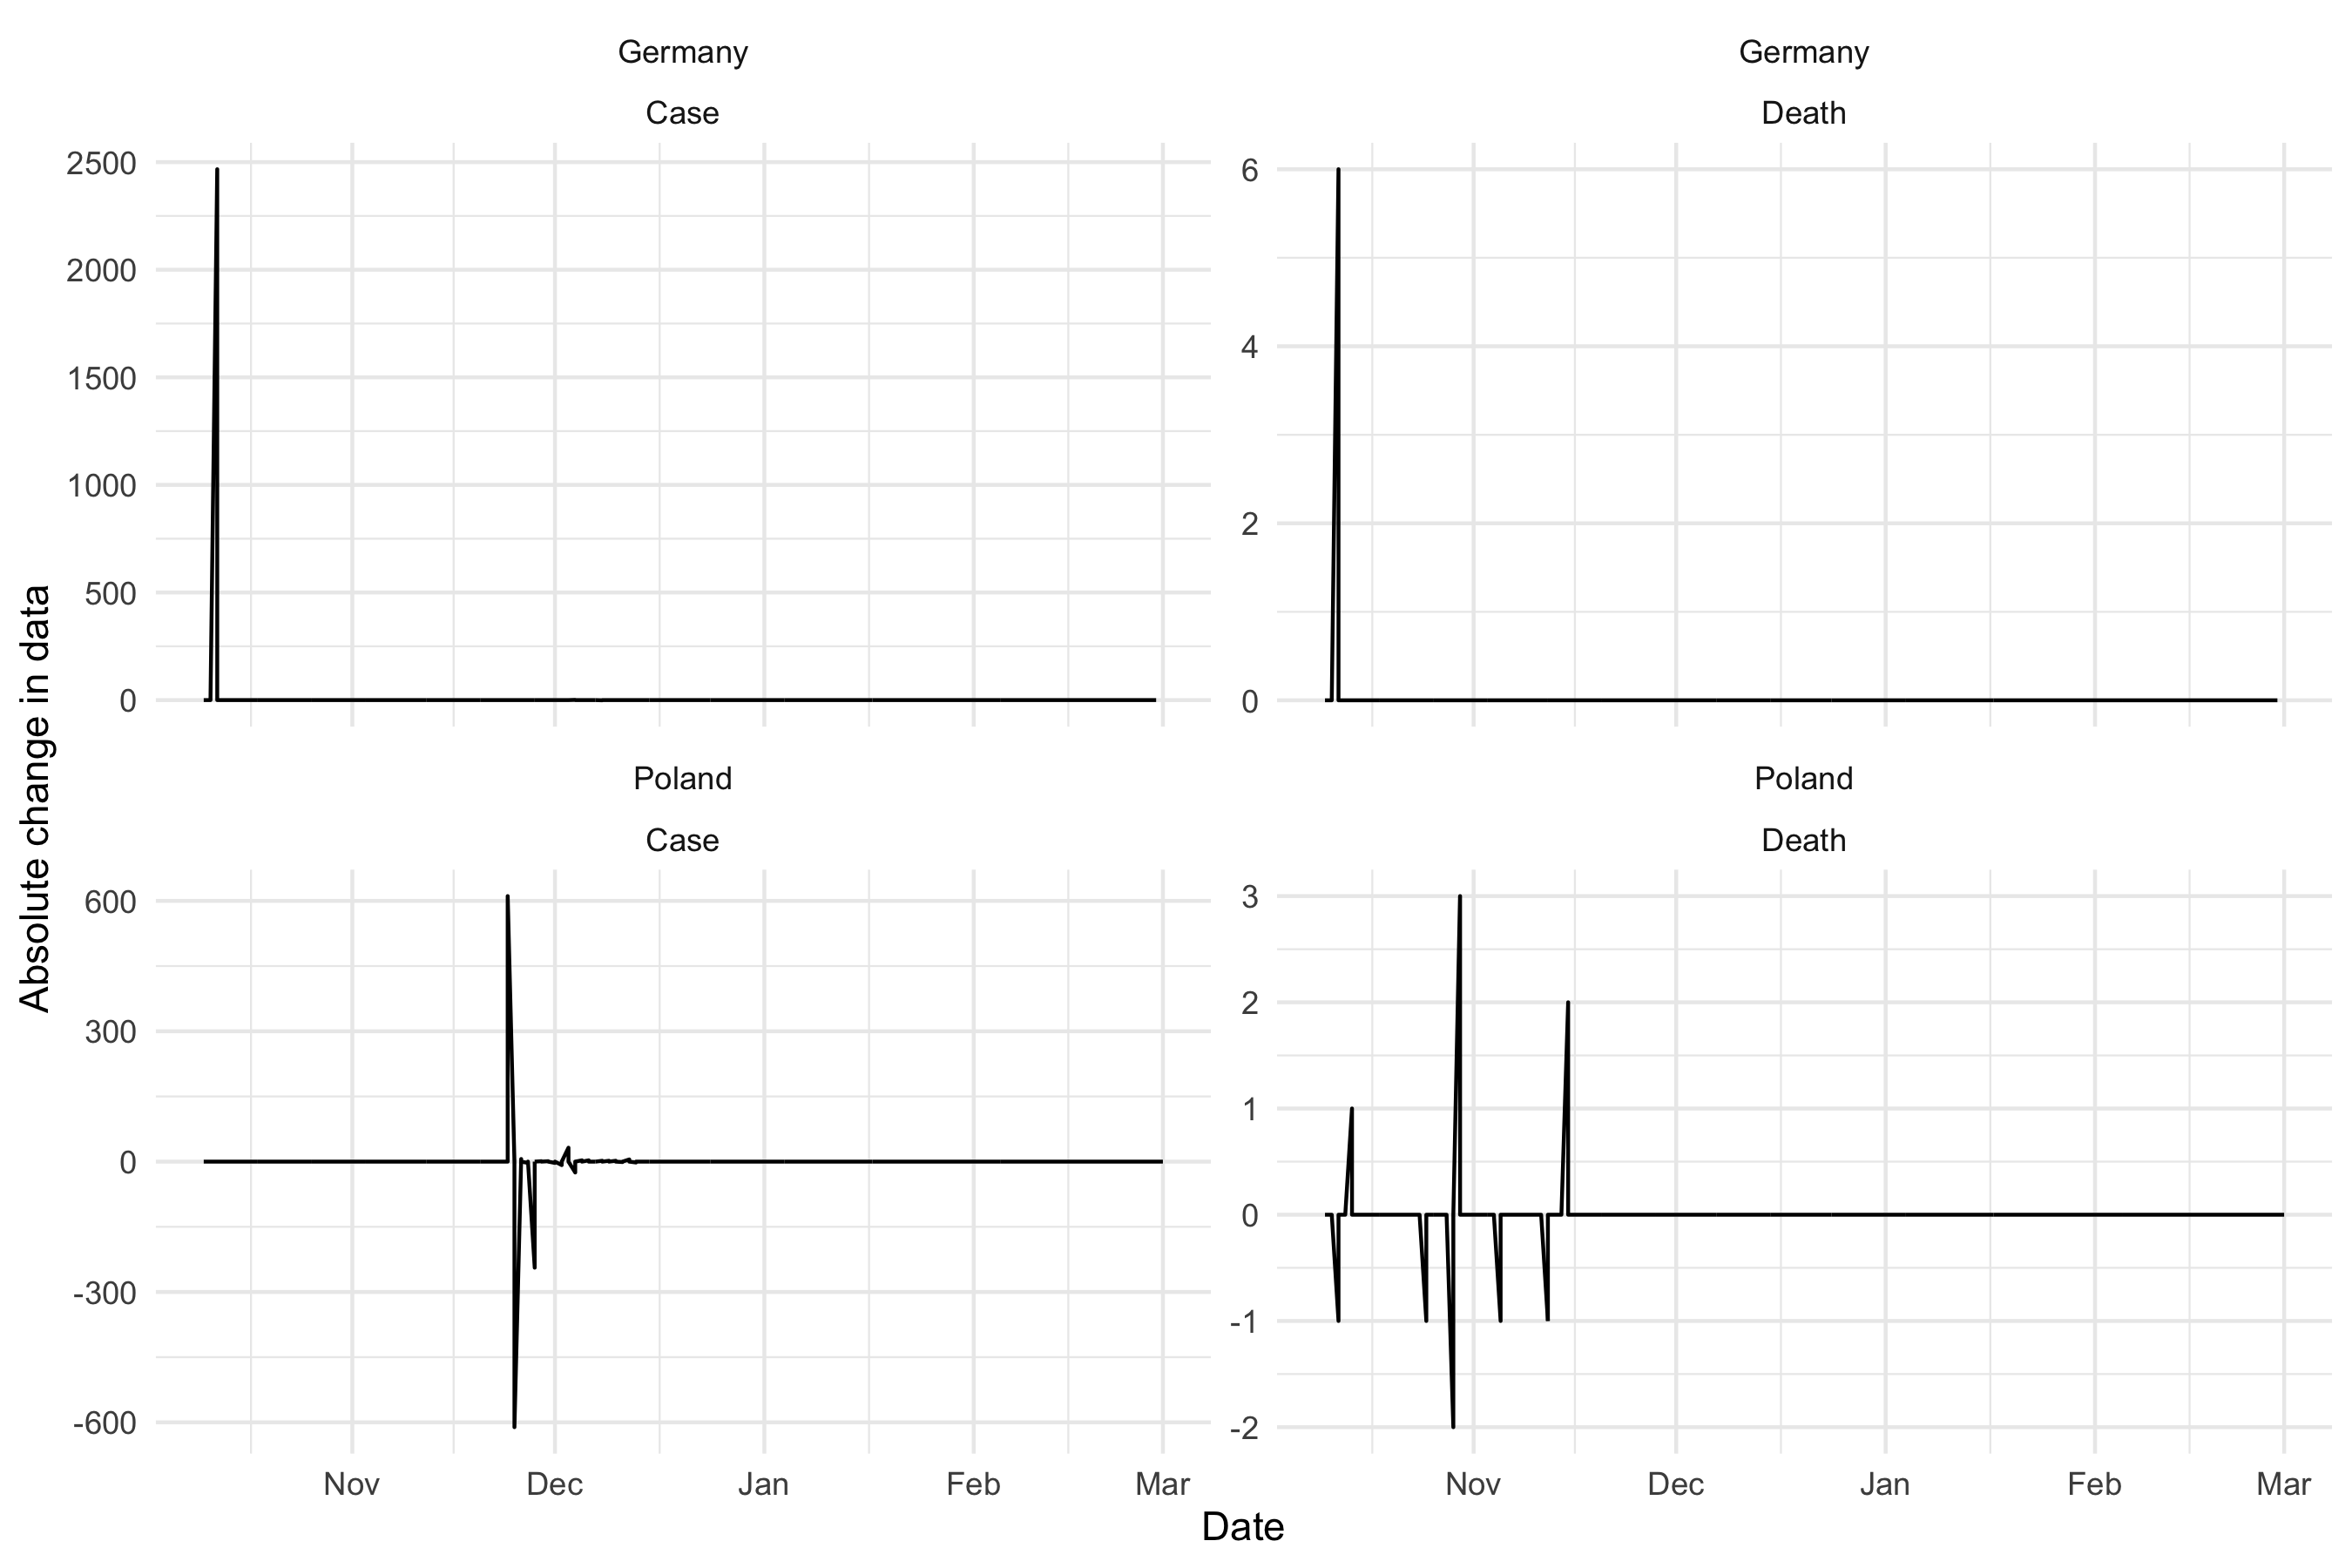
\includegraphics[width=1\linewidth,]{../../../analysis/plots/daily-data-updates}
\caption{Visualisation of the absolute difference between the daily report data at the time and the data now. In Germany, there were zero cases and deaths reported on 2020-10-12, and only later 2467 cases and 6 deaths were added. Data were last accessed through the German and Polish Forecast Hub on May 10 2022.}\label{fig:daily-truth-update}
\end{figure}

\begin{figure}[H]
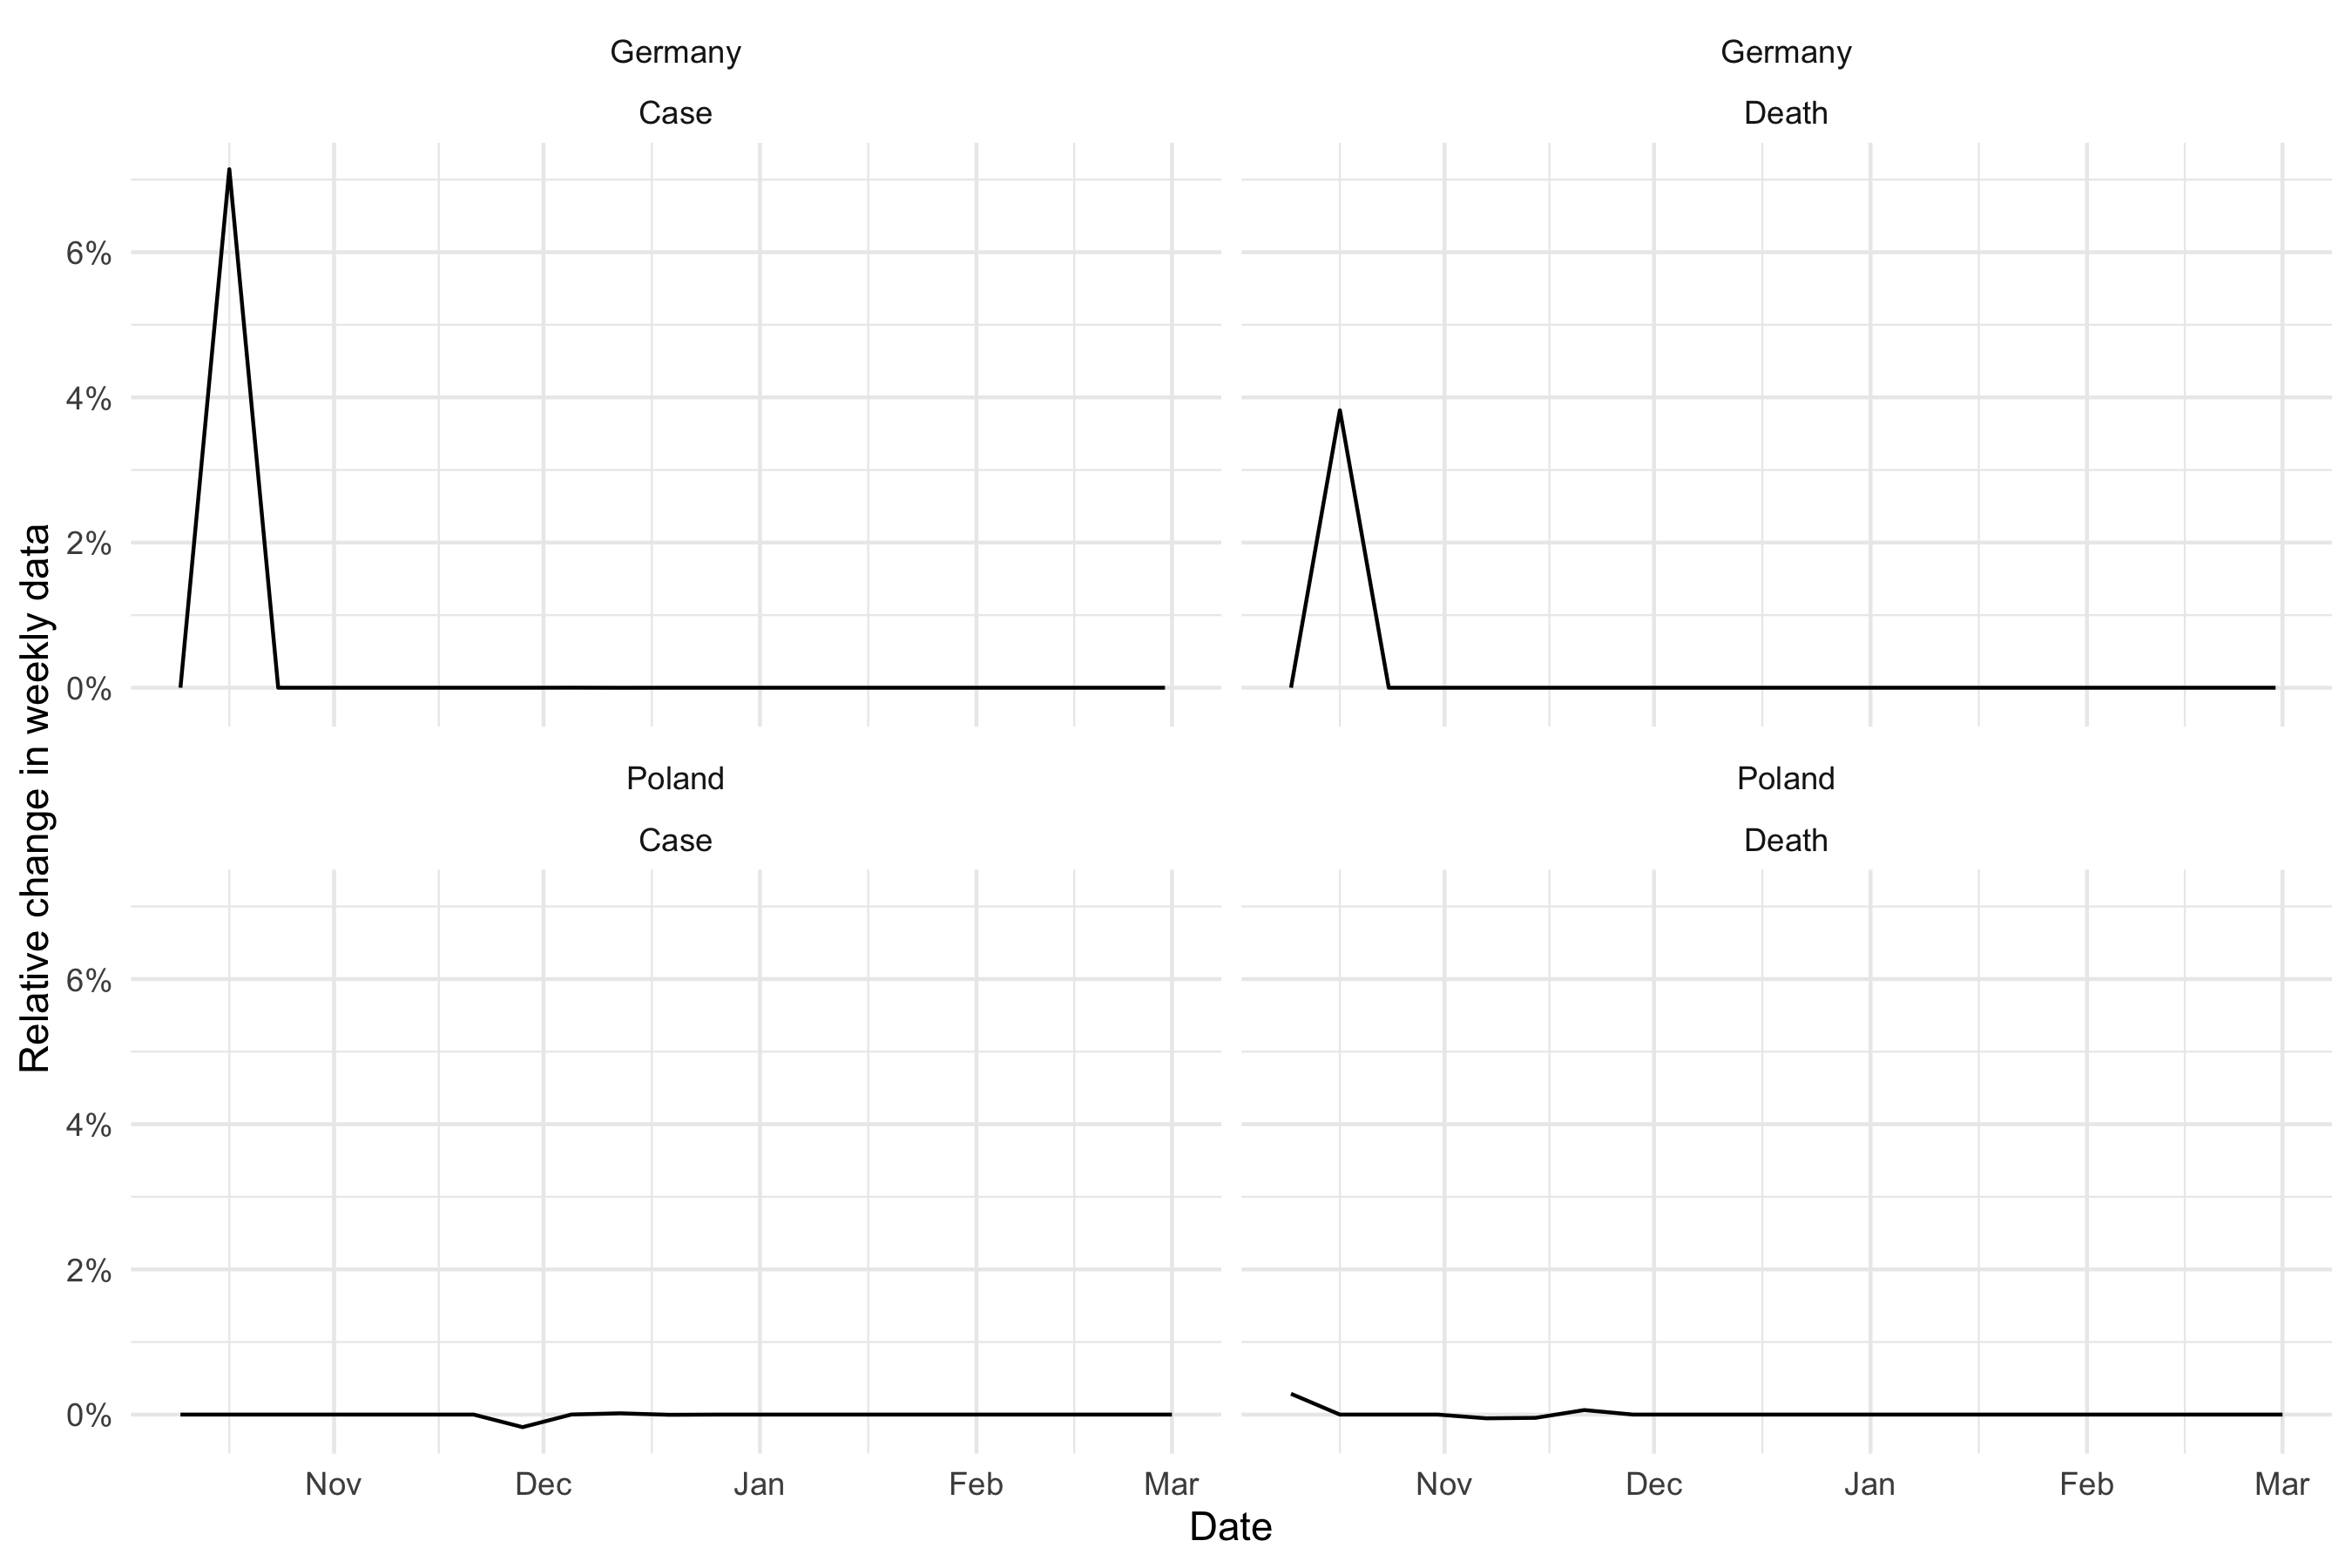
\includegraphics[width=1\linewidth,]{../../../analysis/plots/weekly-data-updates}
\caption{Visualisation of the relative difference between the weekly report data at the time and the data now. Apart from the data that was retrospectively added on 2020-10-12, data updates did not have a noticeable effect on weekly data (as shown in the forecasting application). Data were last accessed through the German and Polish Forecast Hub on May 10 2022.}\label{fig:weekly-truth-update}
\end{figure}

\clearpage

\hypertarget{visualisation-of-scores-and-forecasts-1-3-4-weeks-ahead}{%
\subsection{Visualisation of scores and forecasts 1, 3, 4 weeks
ahead}\label{visualisation-of-scores-and-forecasts-1-3-4-weeks-ahead}}

\begin{figure}[H]
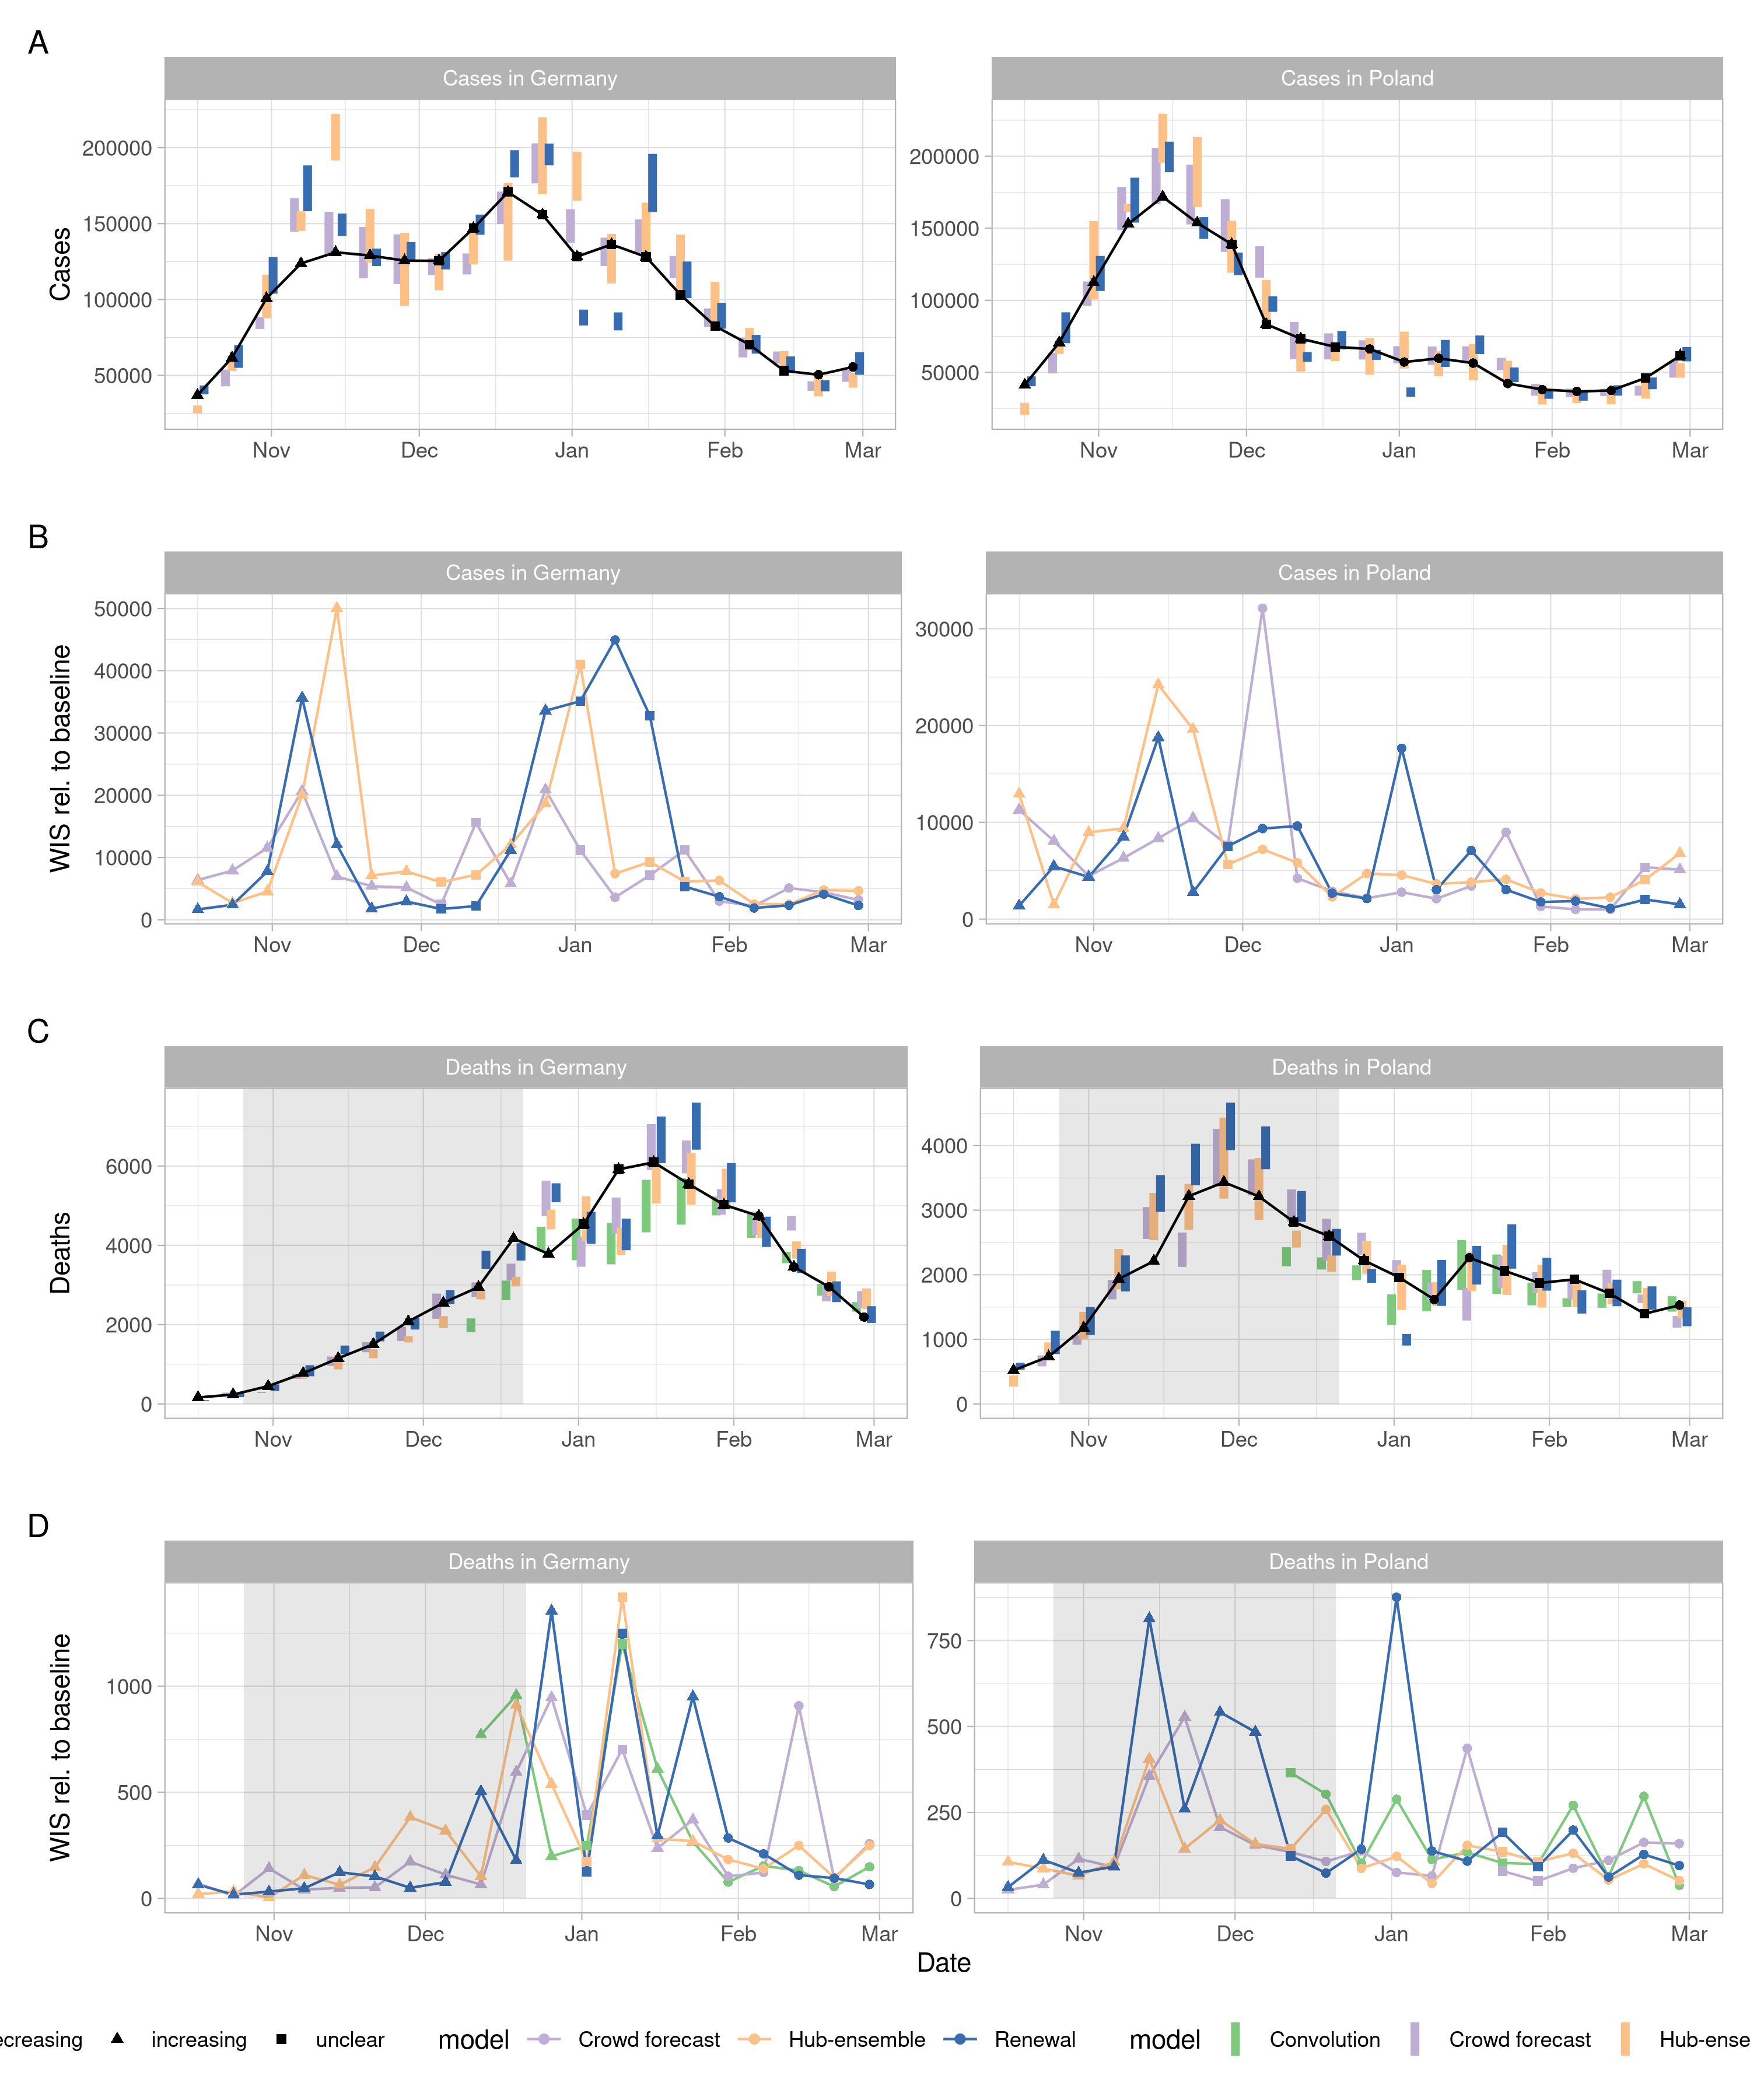
\includegraphics[width=1\linewidth,]{../../../analysis/plots/figure-forecasts-1.png} 
\caption{A, C: Visualisation of 50\% prediction intervals of one week ahead forecasts against the reported values. Forecasts that were not scored (because there was no complete set of death forecasts available) are greyed out. B, D: Visualisation of corresponding WIS.}\label{fig:forecasts-and-truth-1}
\end{figure}

\begin{figure}[H]
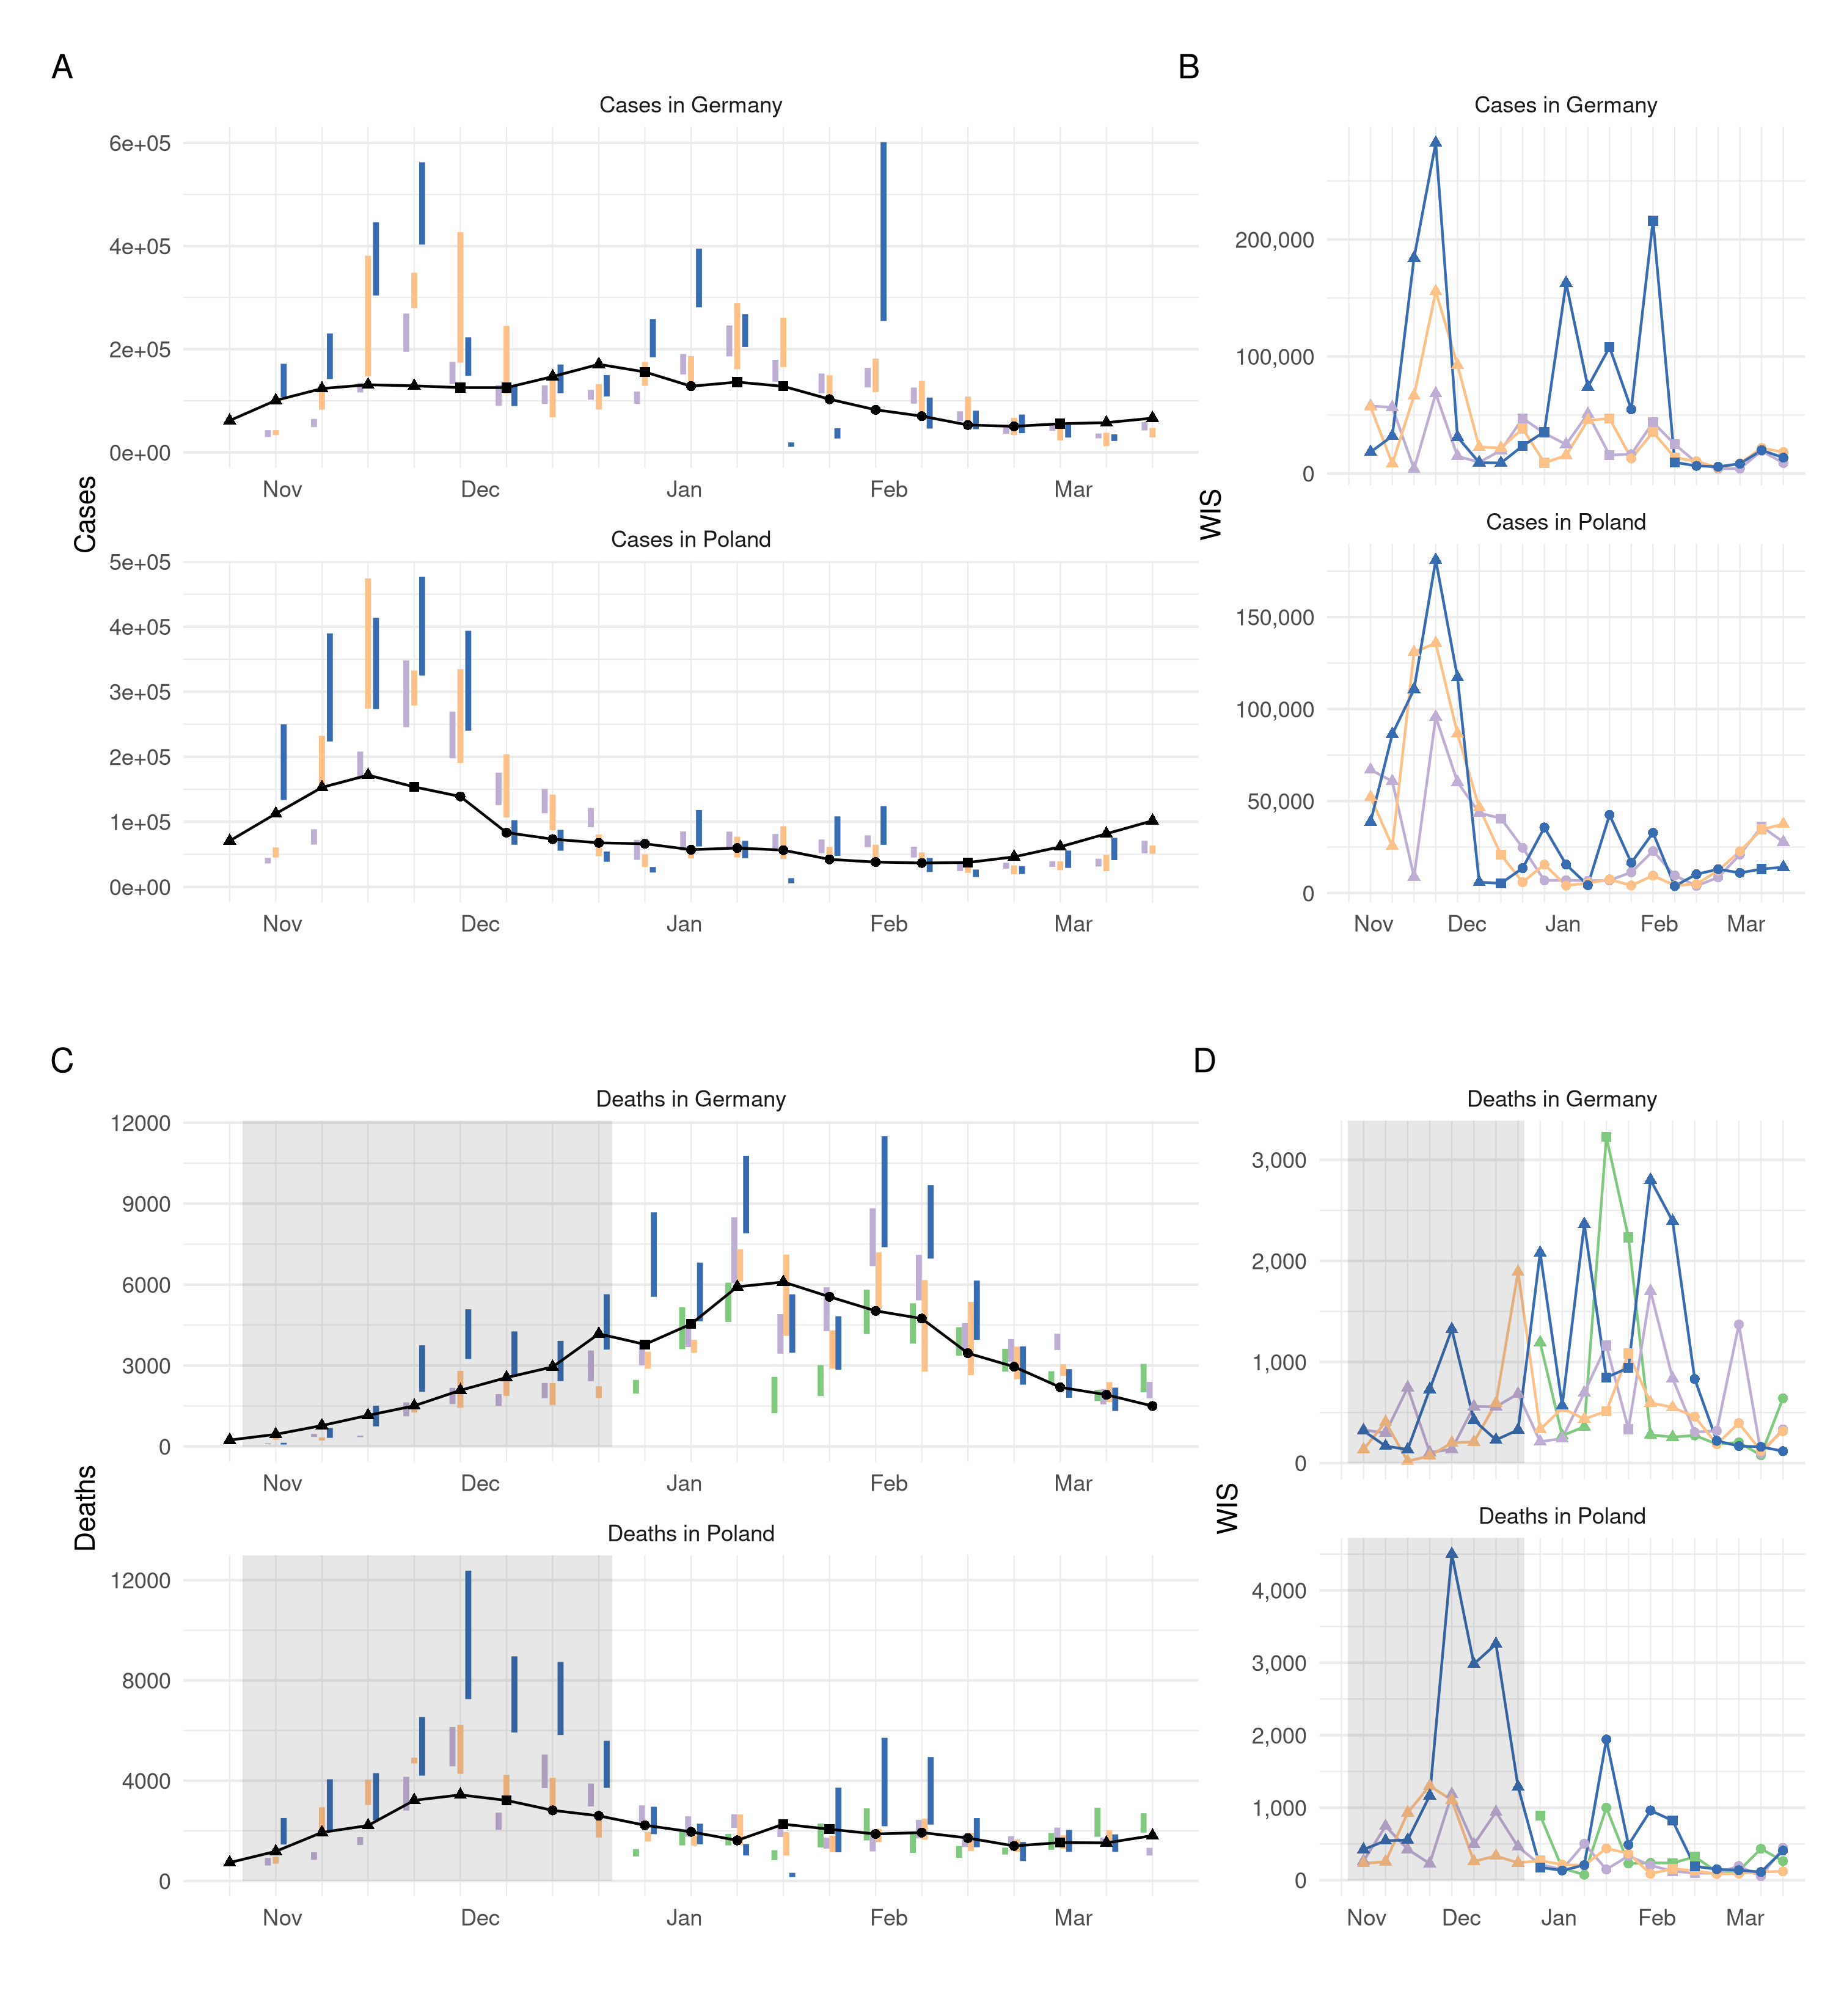
\includegraphics[width=1\linewidth,]{../../../analysis/plots/figure-forecasts-3} 
\caption{A, C: Visualisation of 50\% prediction intervals of three week ahead forecasts against the reported values. Forecasts that were not scored (because there was no complete set of death forecasts available) are greyed out. B, D: Visualisation of corresponding WIS.}\label{fig:forecasts-and-truth-3}
\end{figure}

\begin{figure}[H]
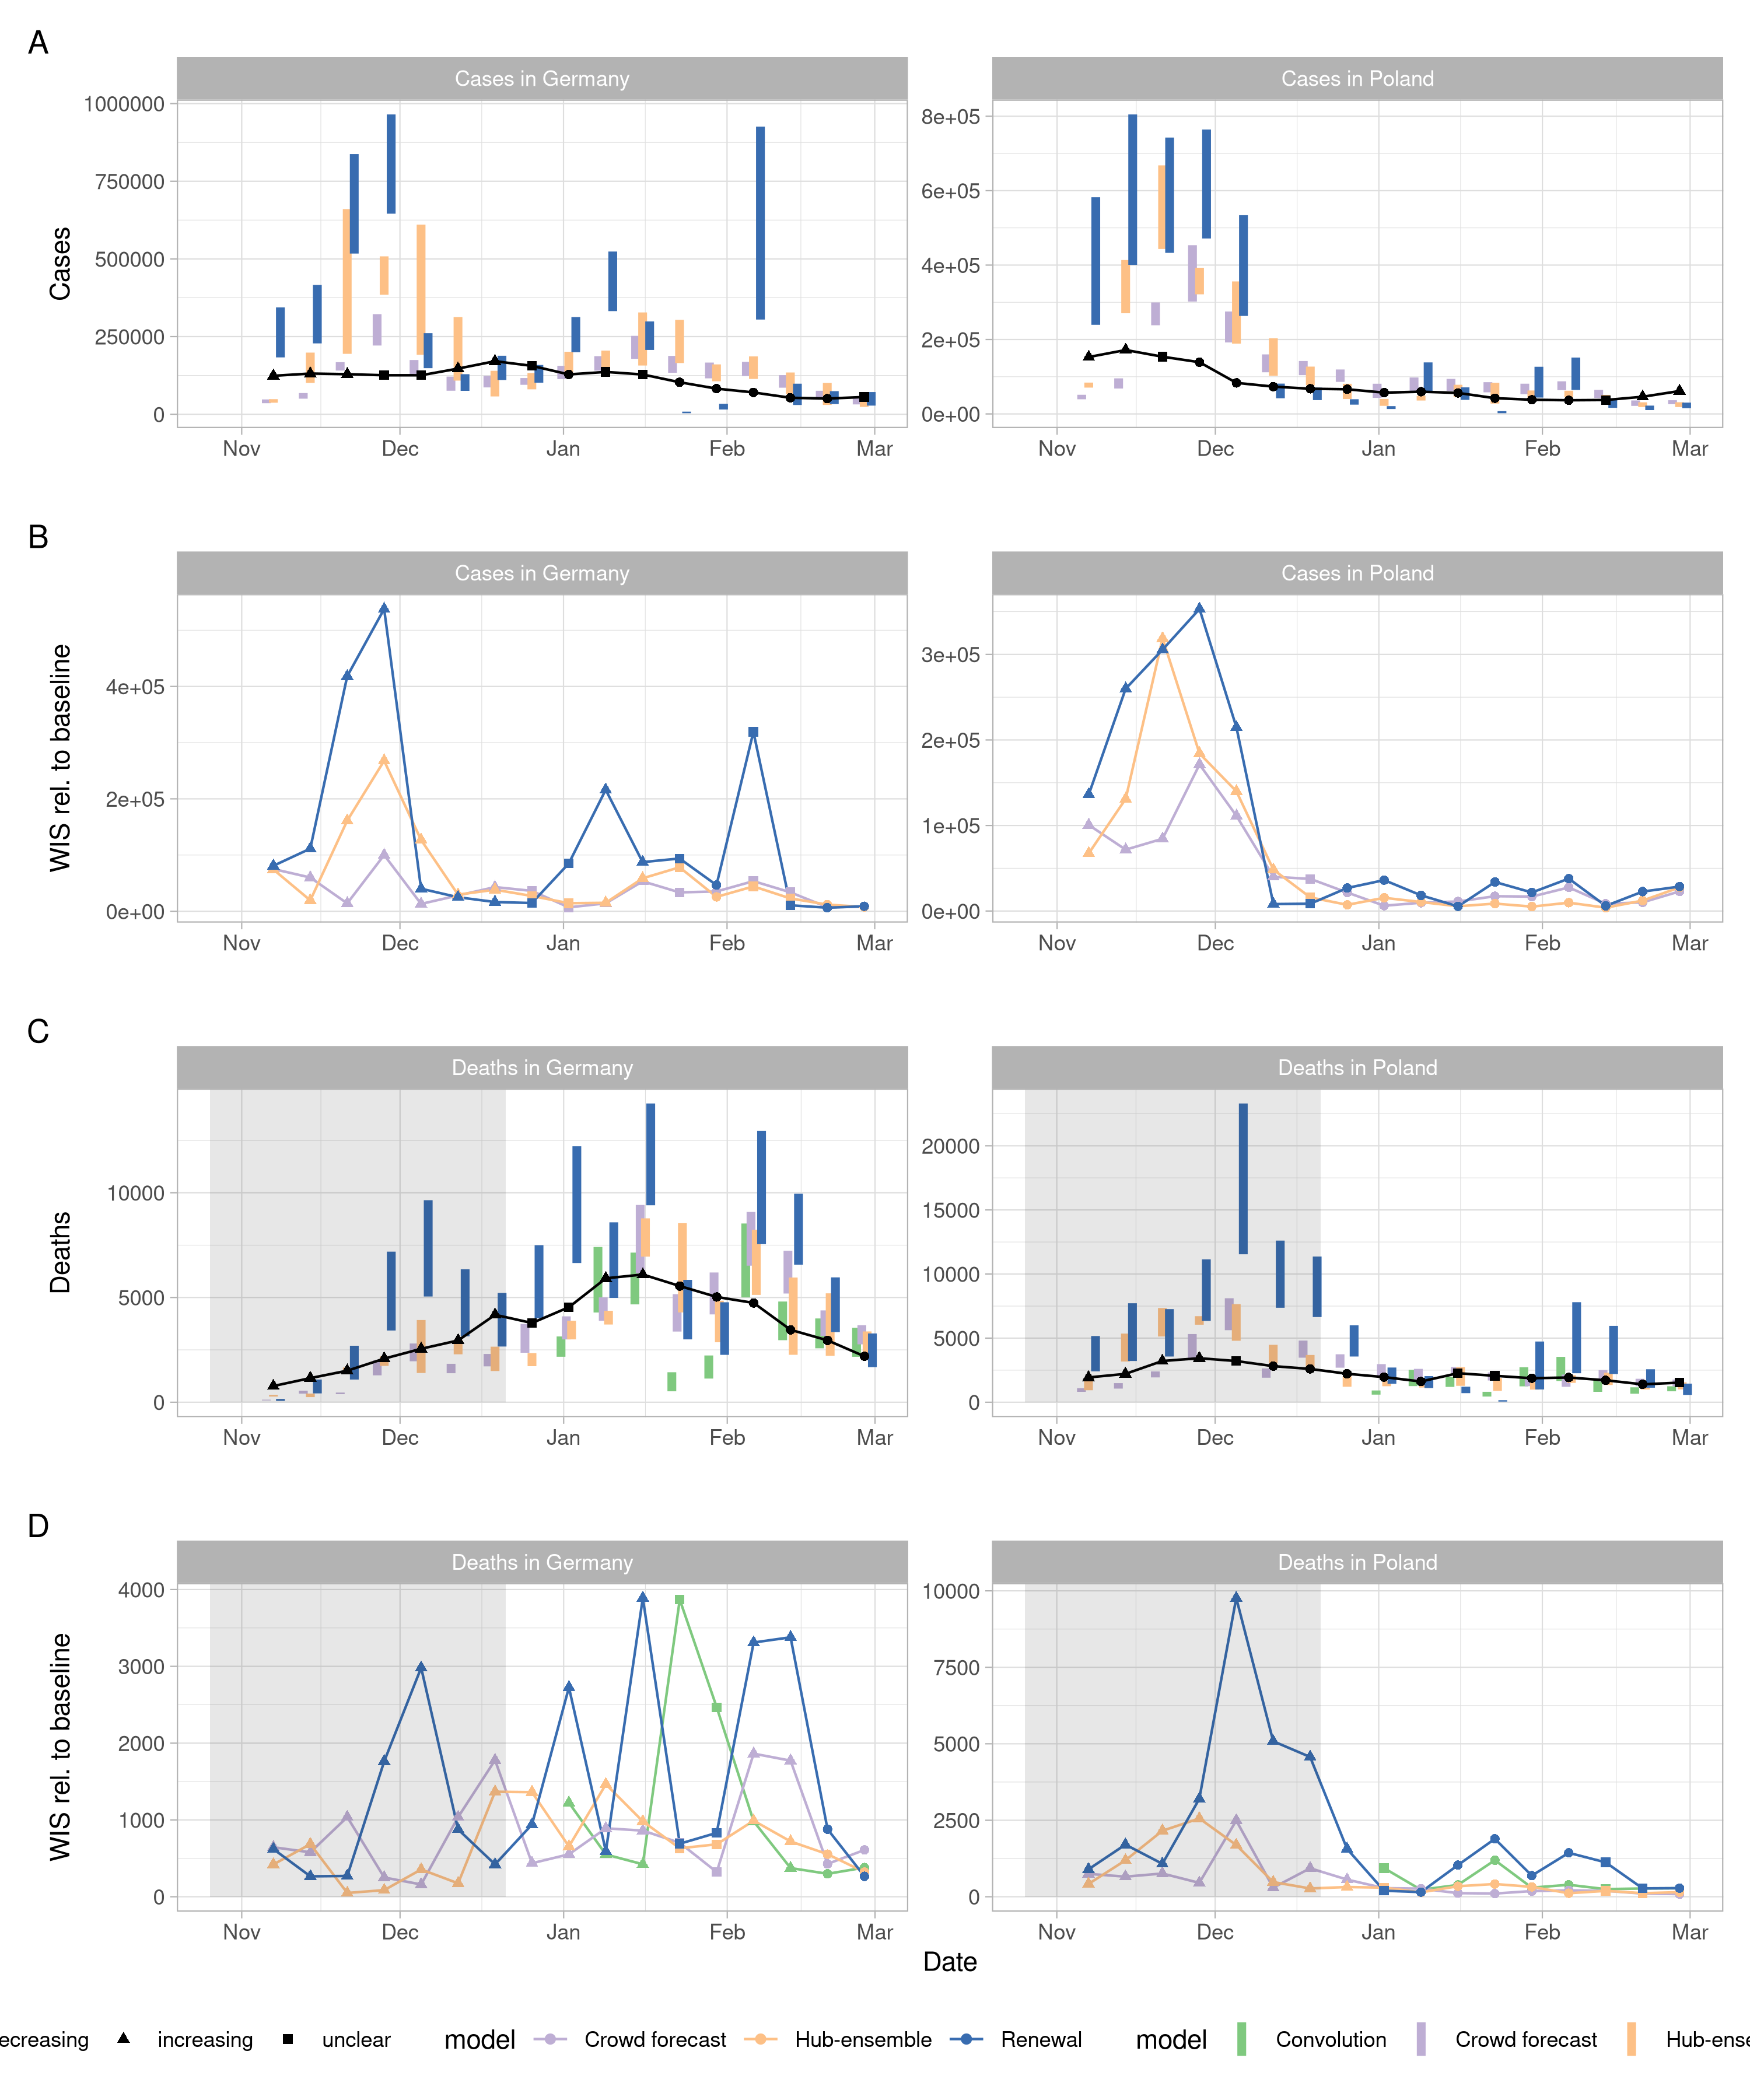
\includegraphics[width=1\linewidth,]{../../../analysis/plots/figure-forecasts-4} 
\caption{A, C: Visualisation of 50\% prediction intervals of four week ahead forecasts against the reported values. Forecasts that were not scored (because there was no complete set of death forecasts available) are greyed out. B, D: Visualisation of corresponding WIS.}\label{fig:forecasts-and-truth-4}
\end{figure}

\clearpage

\hypertarget{distribution-of-scores}{%
\subsection{Distribution of scores}\label{distribution-of-scores}}

\hypertarget{absolute-scores}{%
\subsubsection{Absolute scores}\label{absolute-scores}}

\begin{figure}[H]
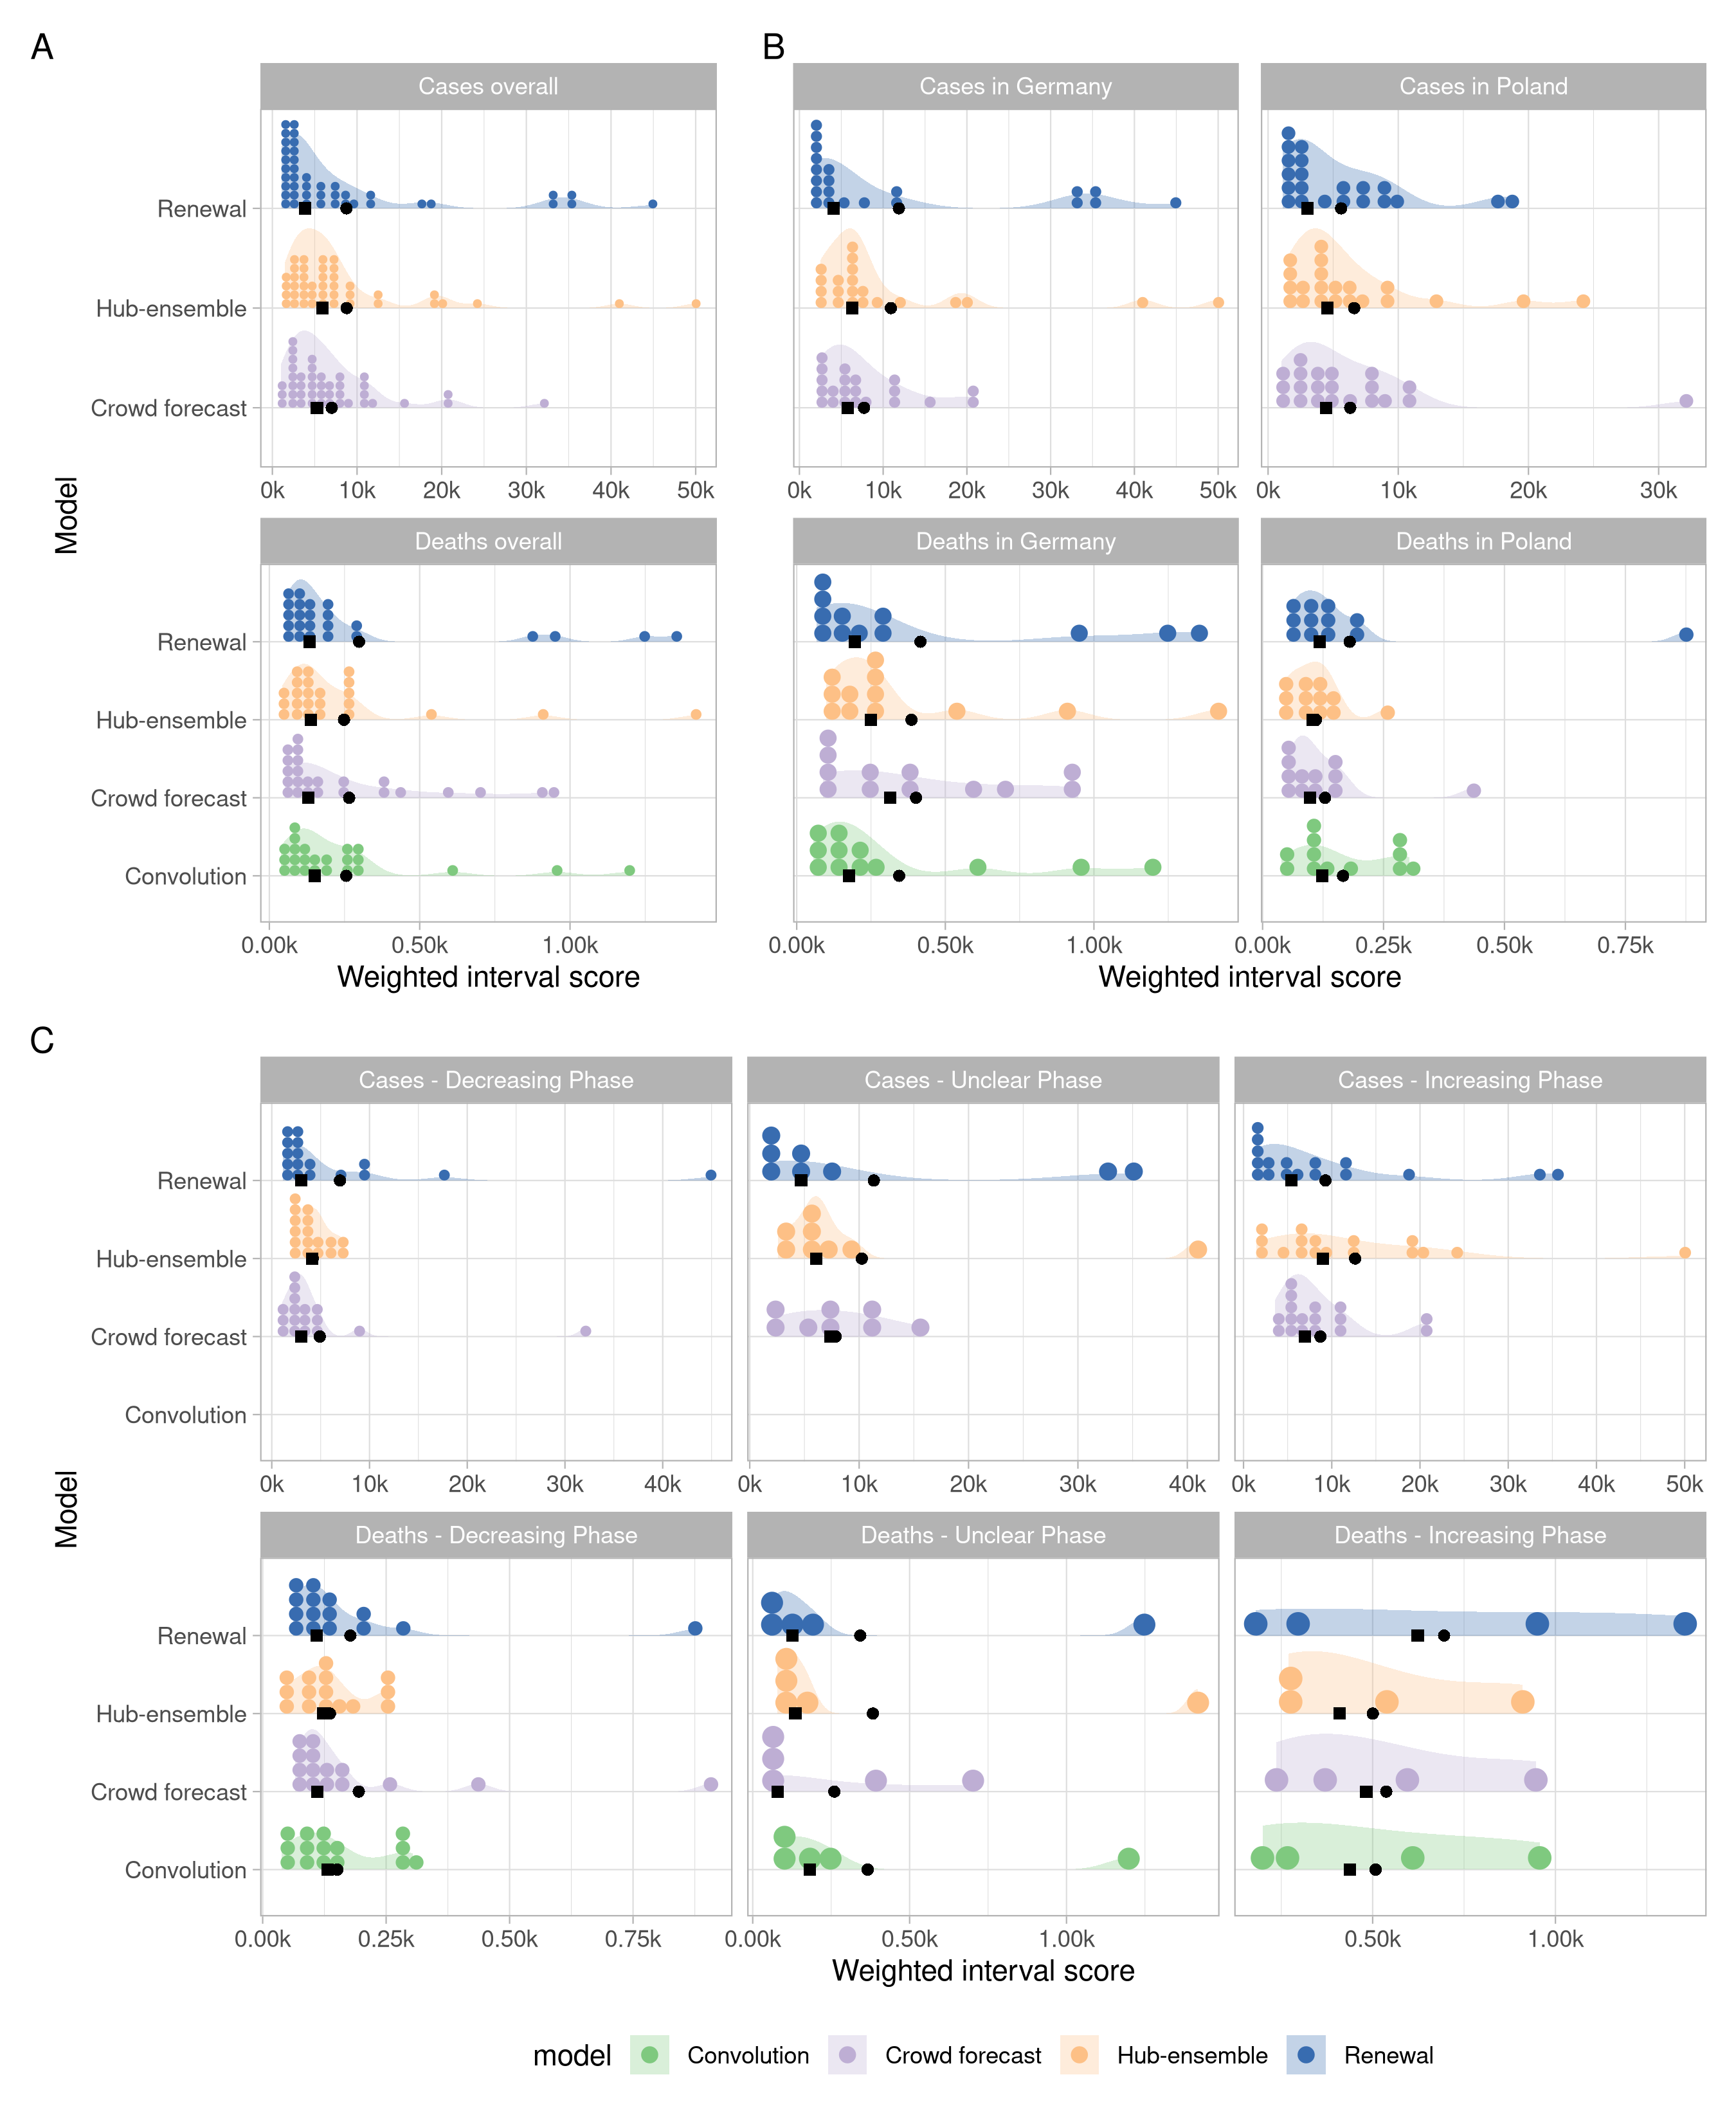
\includegraphics[width=1\linewidth,]{../../../analysis/plots/distribution_scores_wis-1} 
\caption{A: Distribution of weighted interval scores for one week ahead forecasts of the different models and forecast targets. B: Distribution of WIS separate by country.}\label{fig:distribution-scores-1}
\end{figure}

\begin{figure}[H]
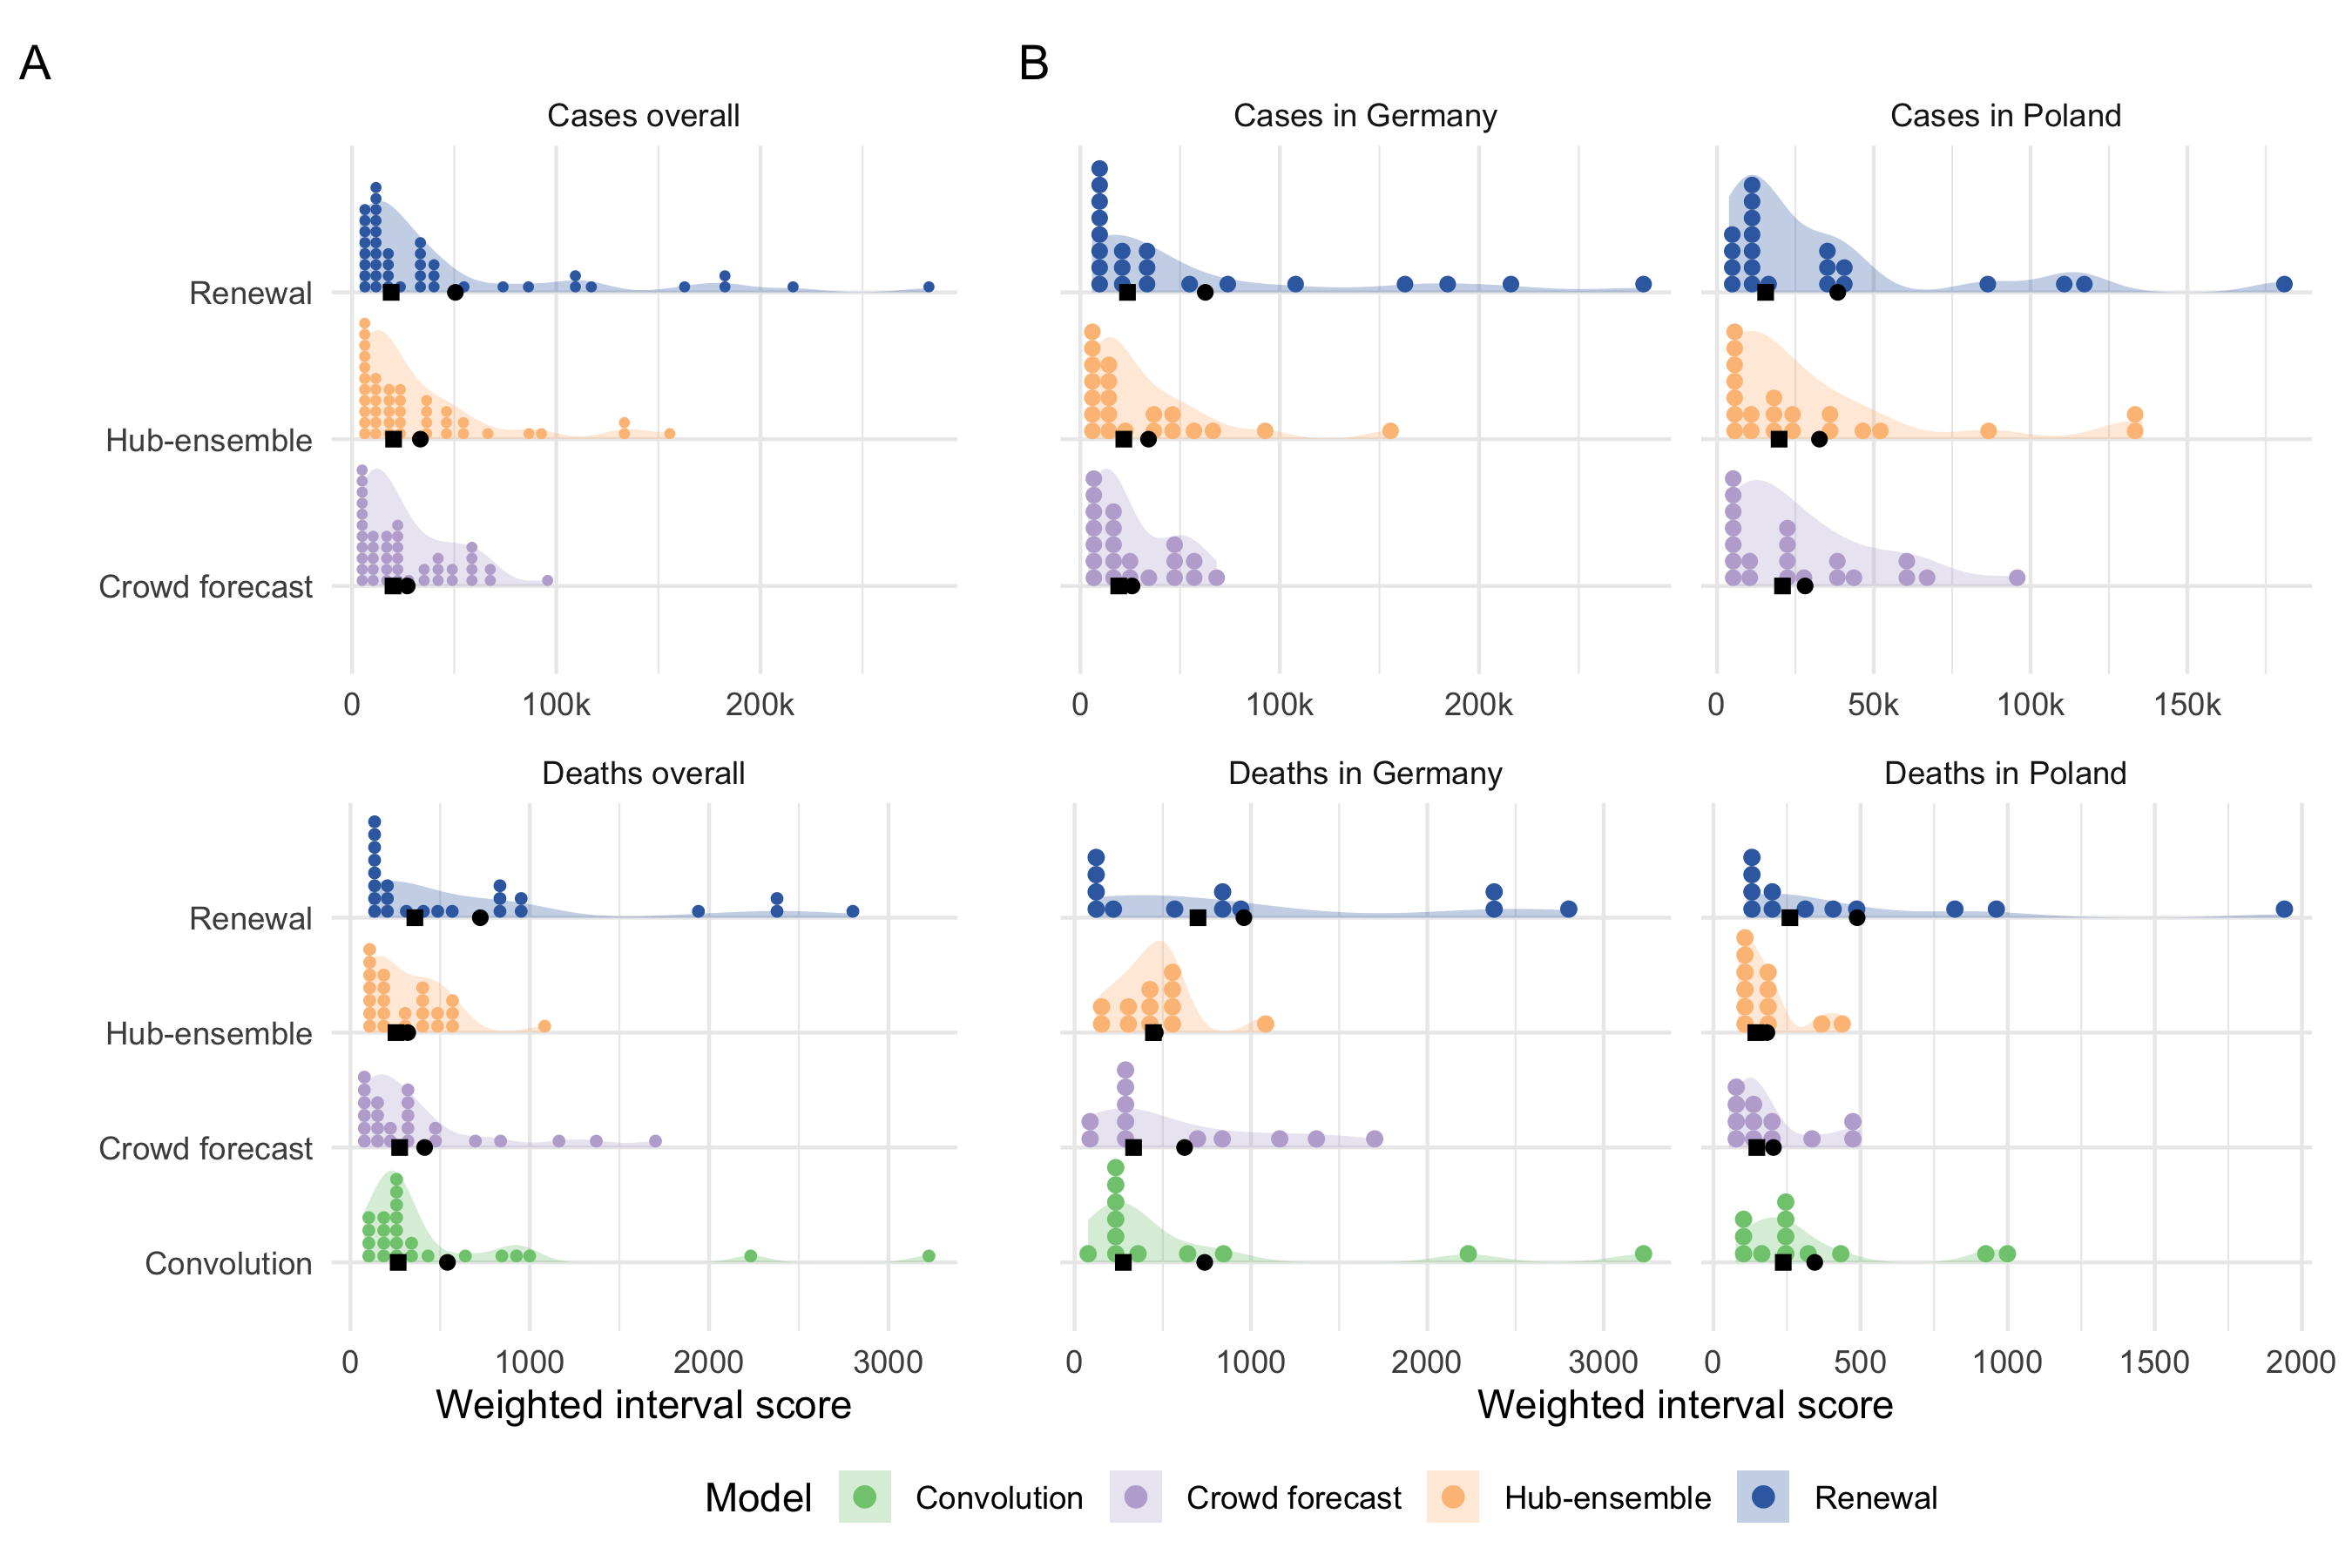
\includegraphics[width=1\linewidth,]{../../../analysis/plots/distribution_scores_wis-3} 
\caption{A: Distribution of weighted interval scores for three week ahead forecasts of the different models and forecast targets. B: Distribution of WIS separate by country.}\label{fig:distribution-scores-3}
\end{figure}

\begin{figure}[H]
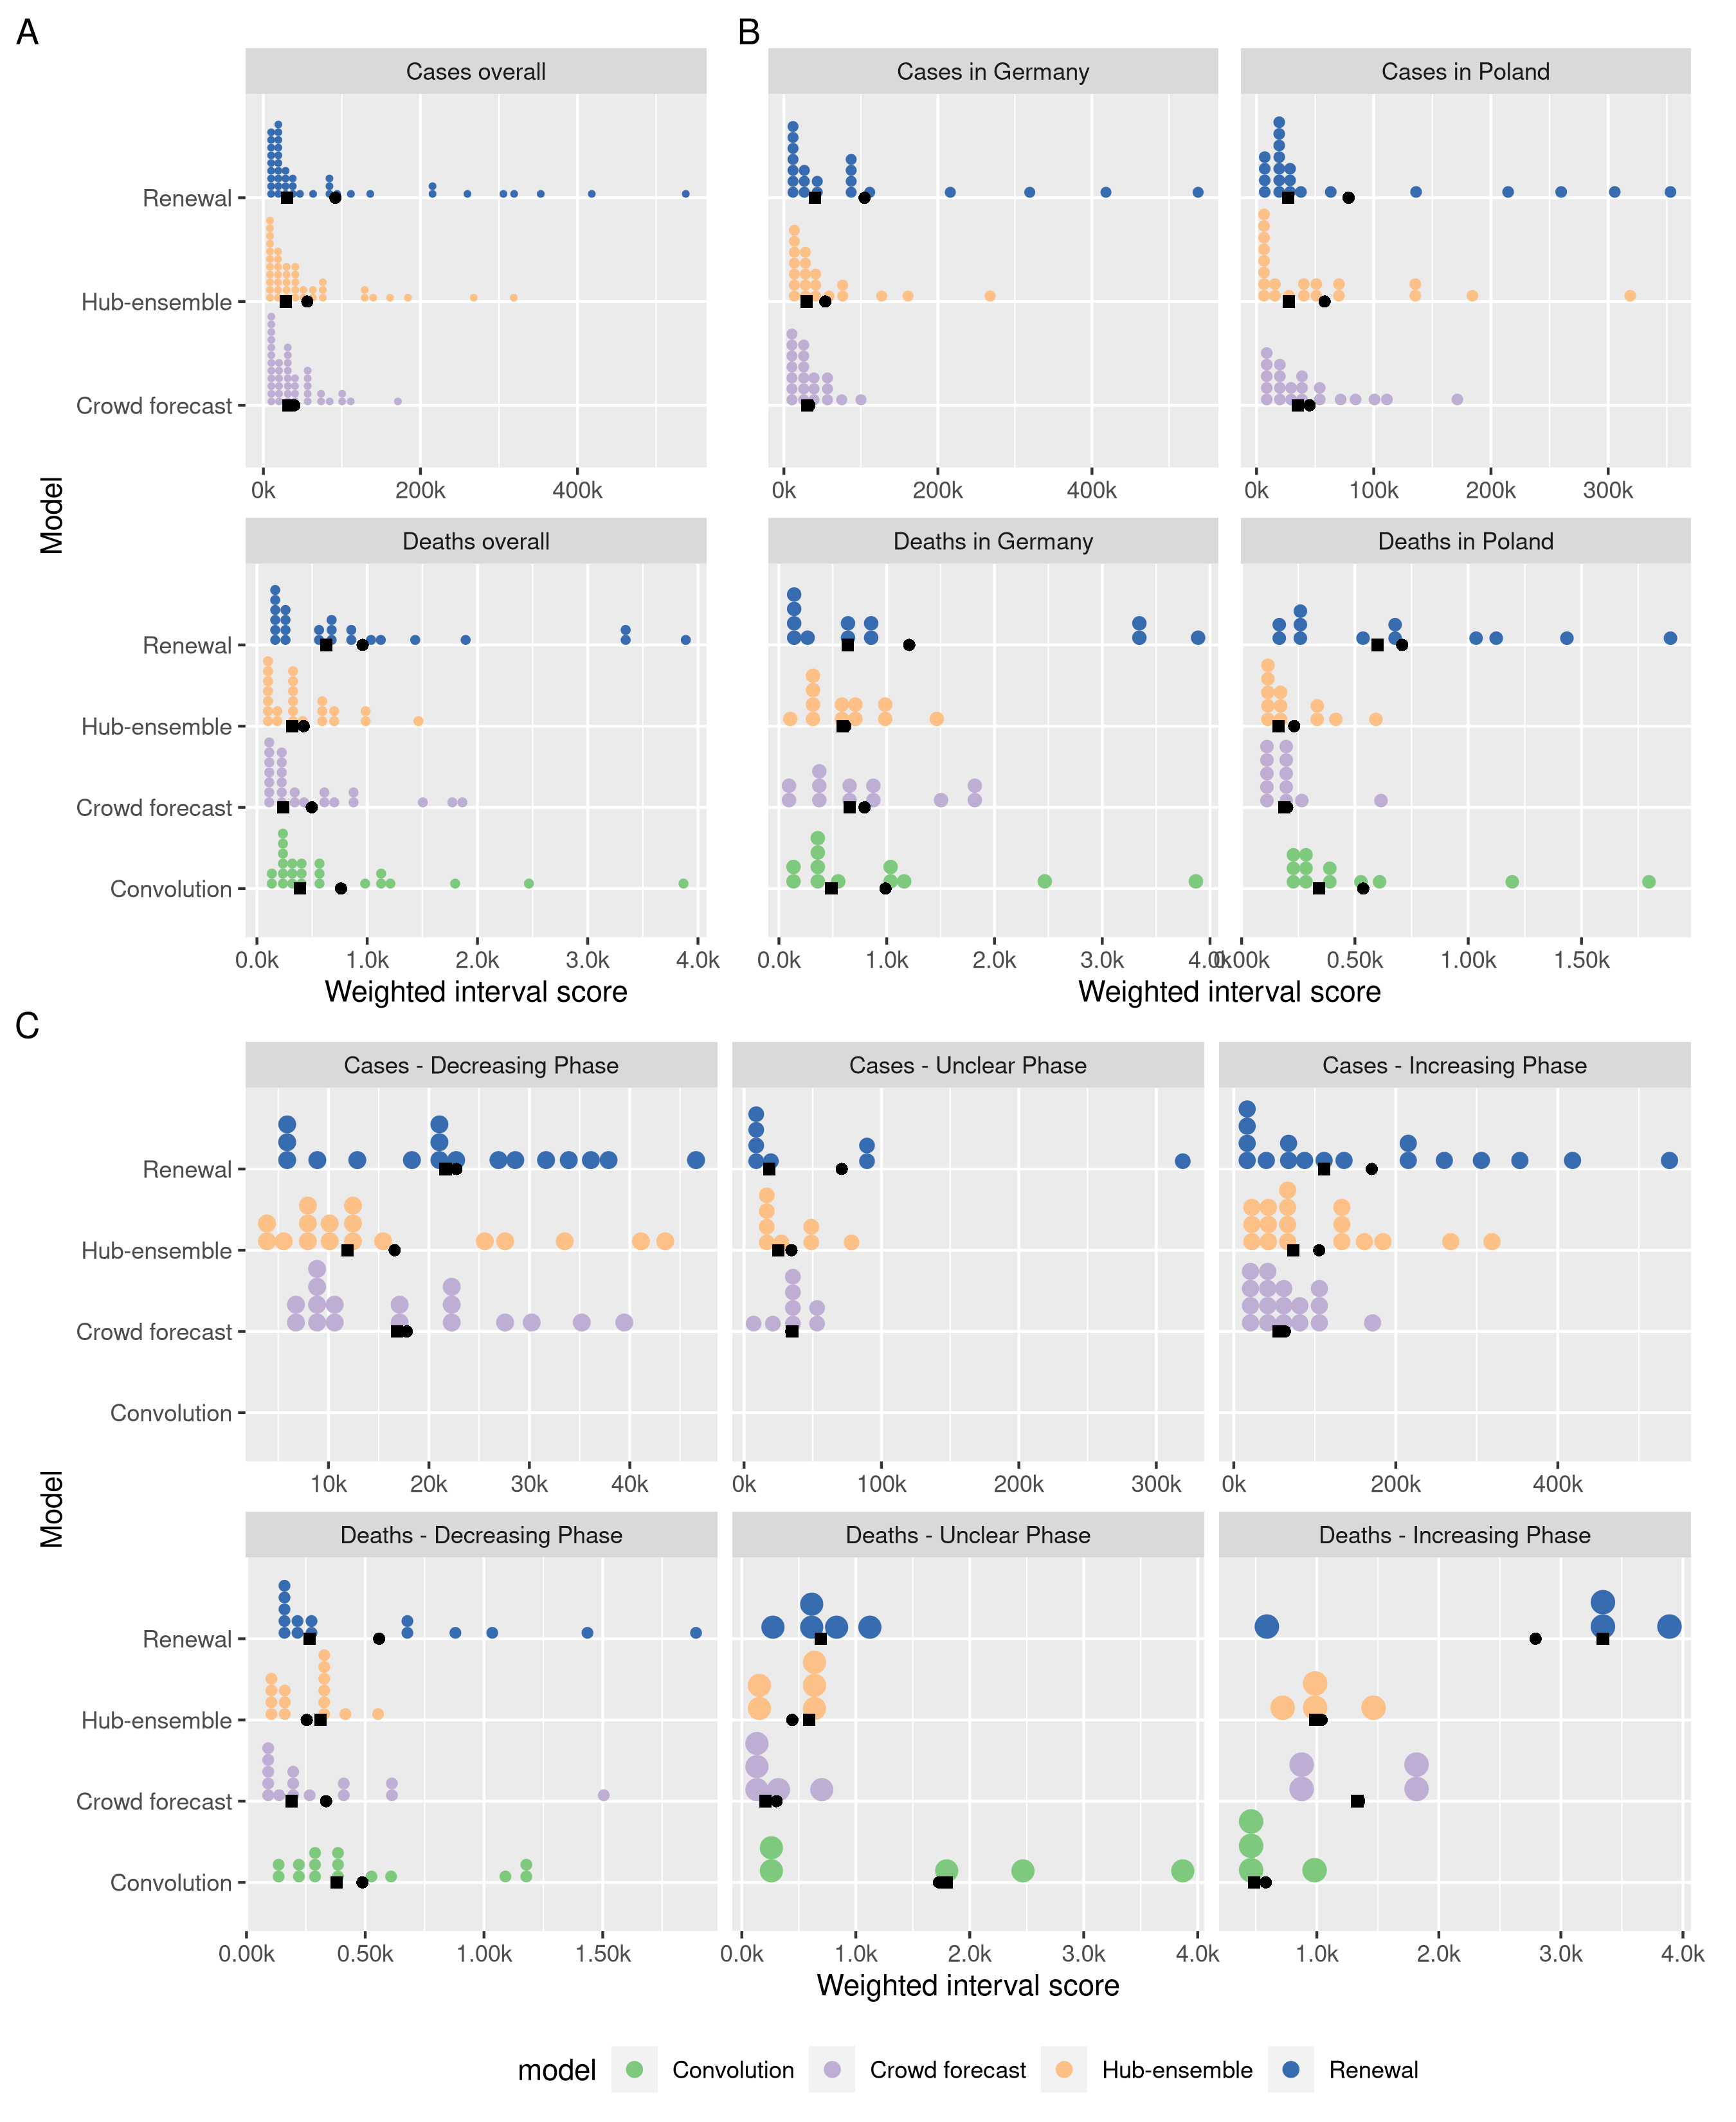
\includegraphics[width=1\linewidth,]{../../../analysis/plots/distribution_scores_wis-4} 
\caption{A: Distribution of weighted interval scores for four week ahead forecasts of the different models and forecast targets. B: Distribution of WIS separate by country.}\label{fig:distribution-scores-4}
\end{figure}

\hypertarget{ranks-achieved-by-forecasts}{%
\subsubsection{Ranks achieved by
forecasts}\label{ranks-achieved-by-forecasts}}

\begin{figure}[H]
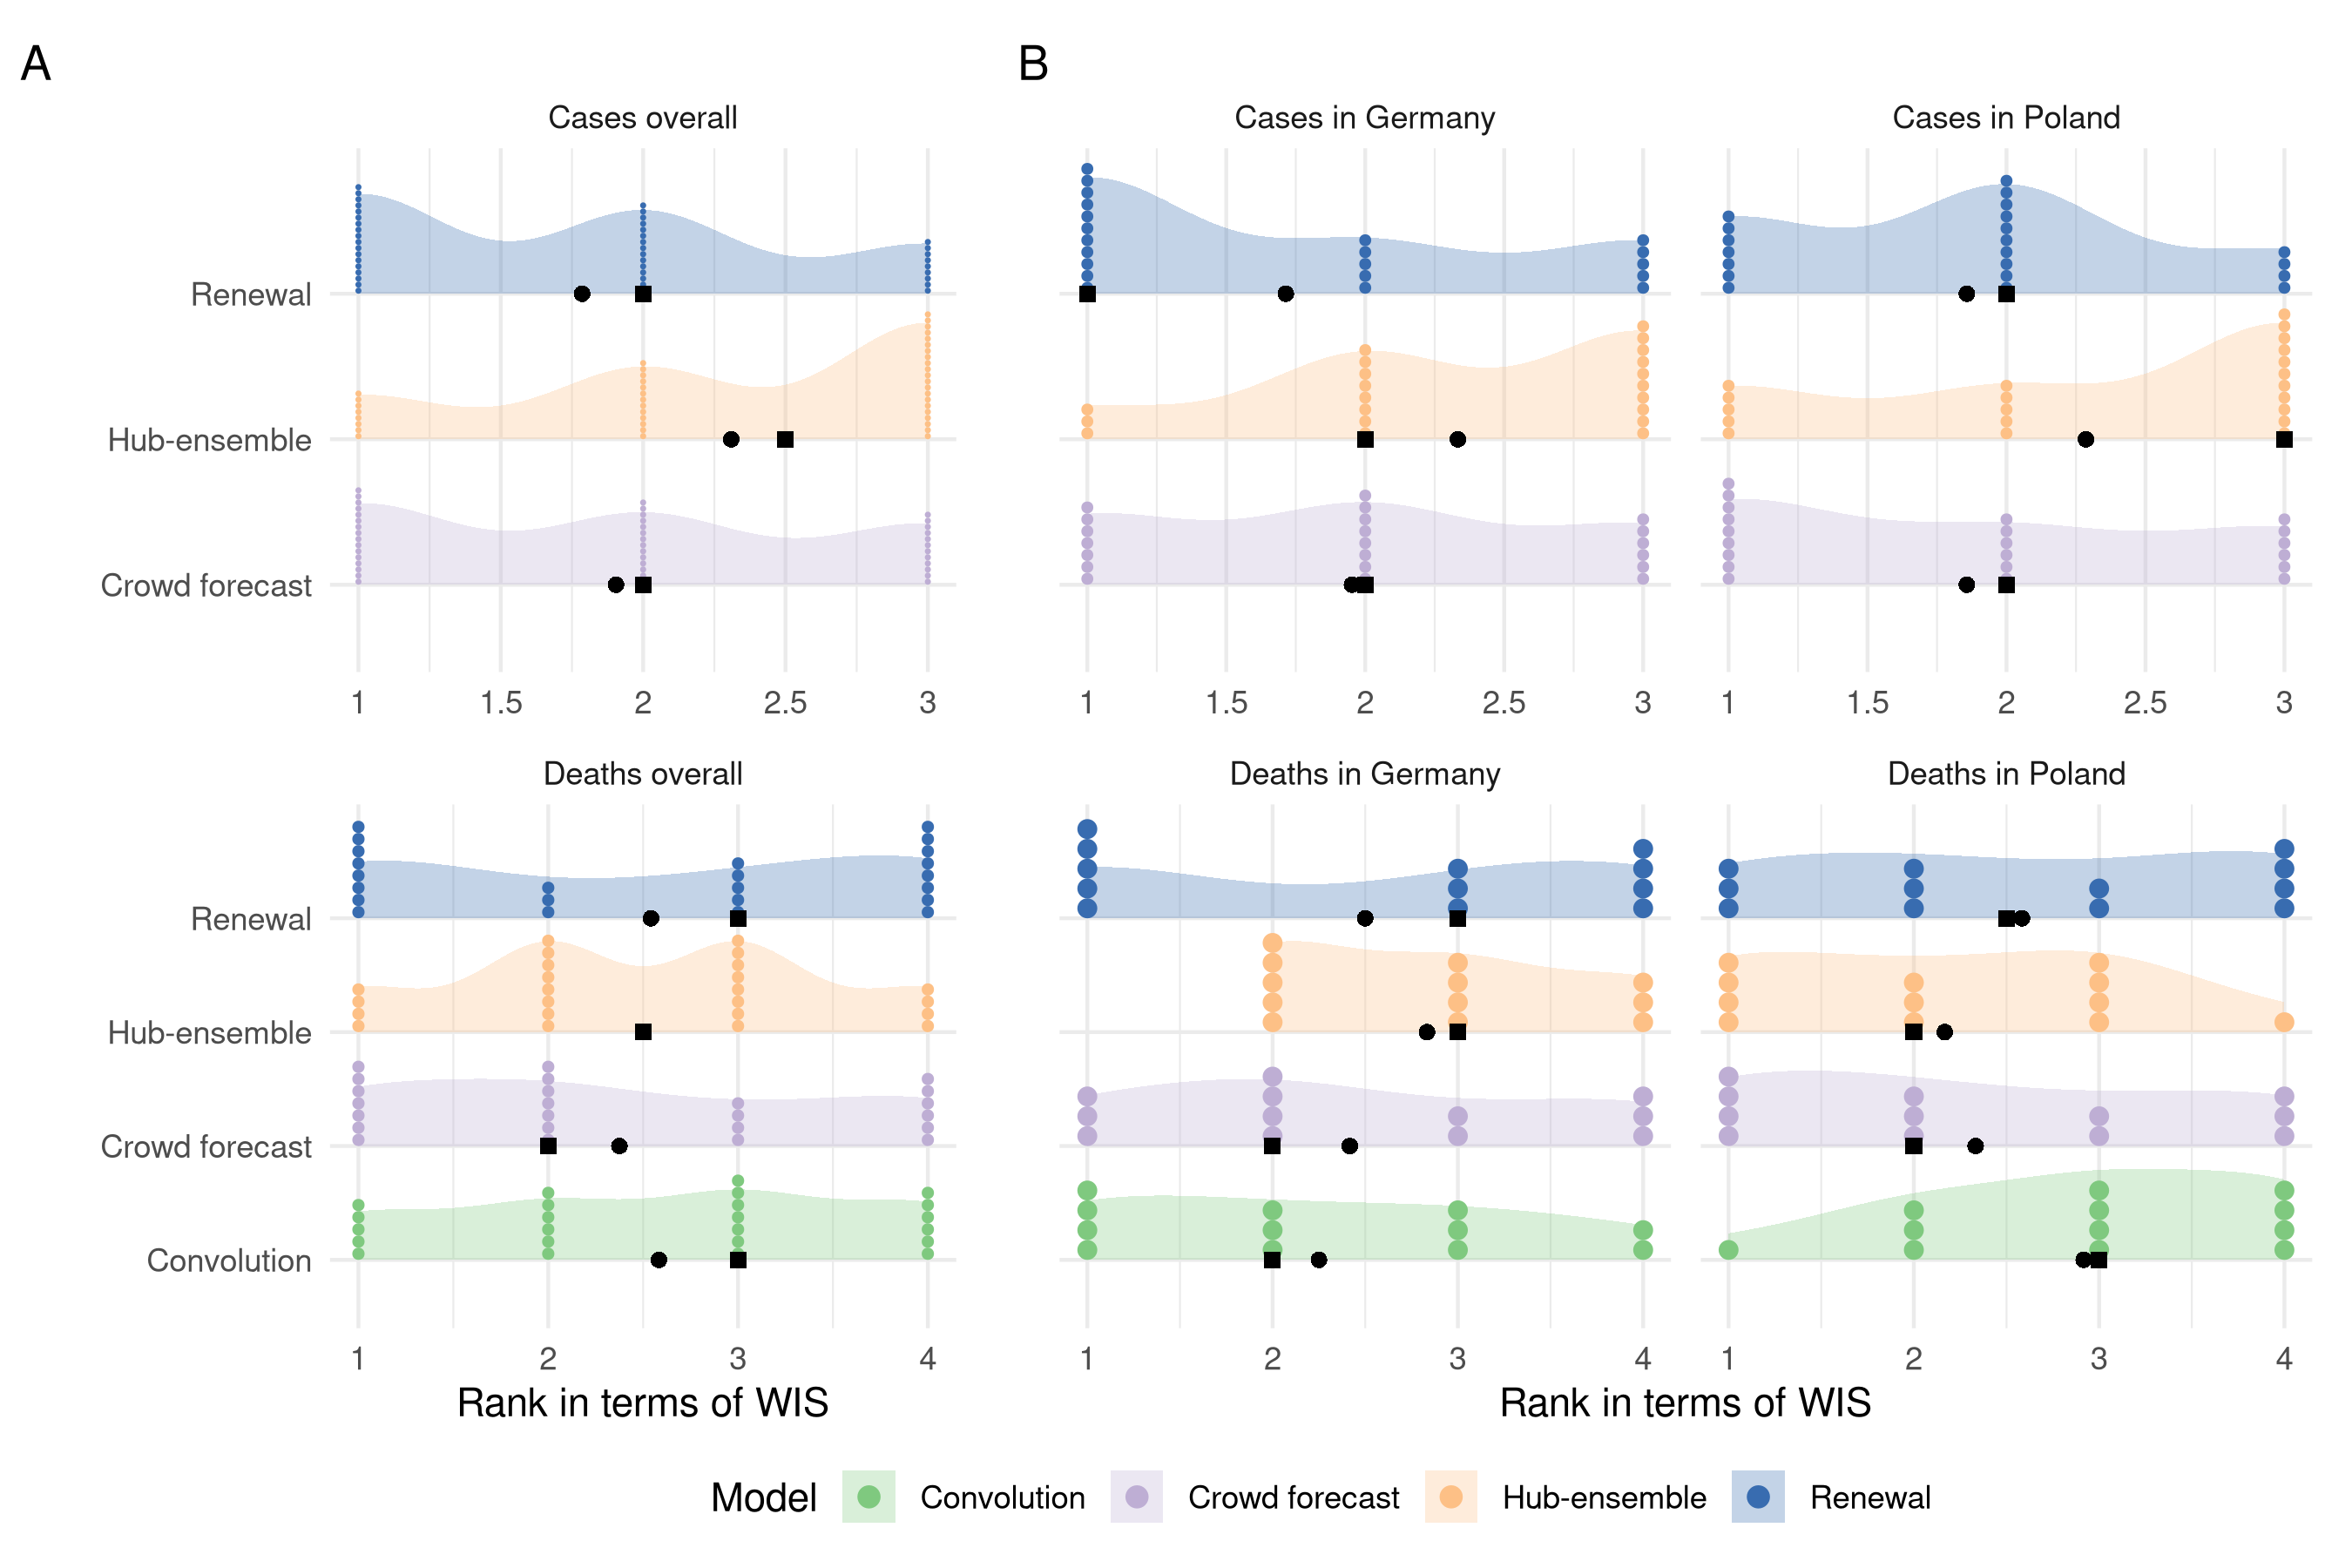
\includegraphics[width=1\linewidth,]{../../../analysis/plots/distribution_scores_wis-1-ranks} 
\caption{A: Distribution of the ranks (determined by the weighted interval score) for one week ahead forecasts of the different models and forecast targets. B: Distribution of ranks separate by country.}\label{fig:distribution-scores-ranks-1}
\end{figure}

\begin{figure}[H]
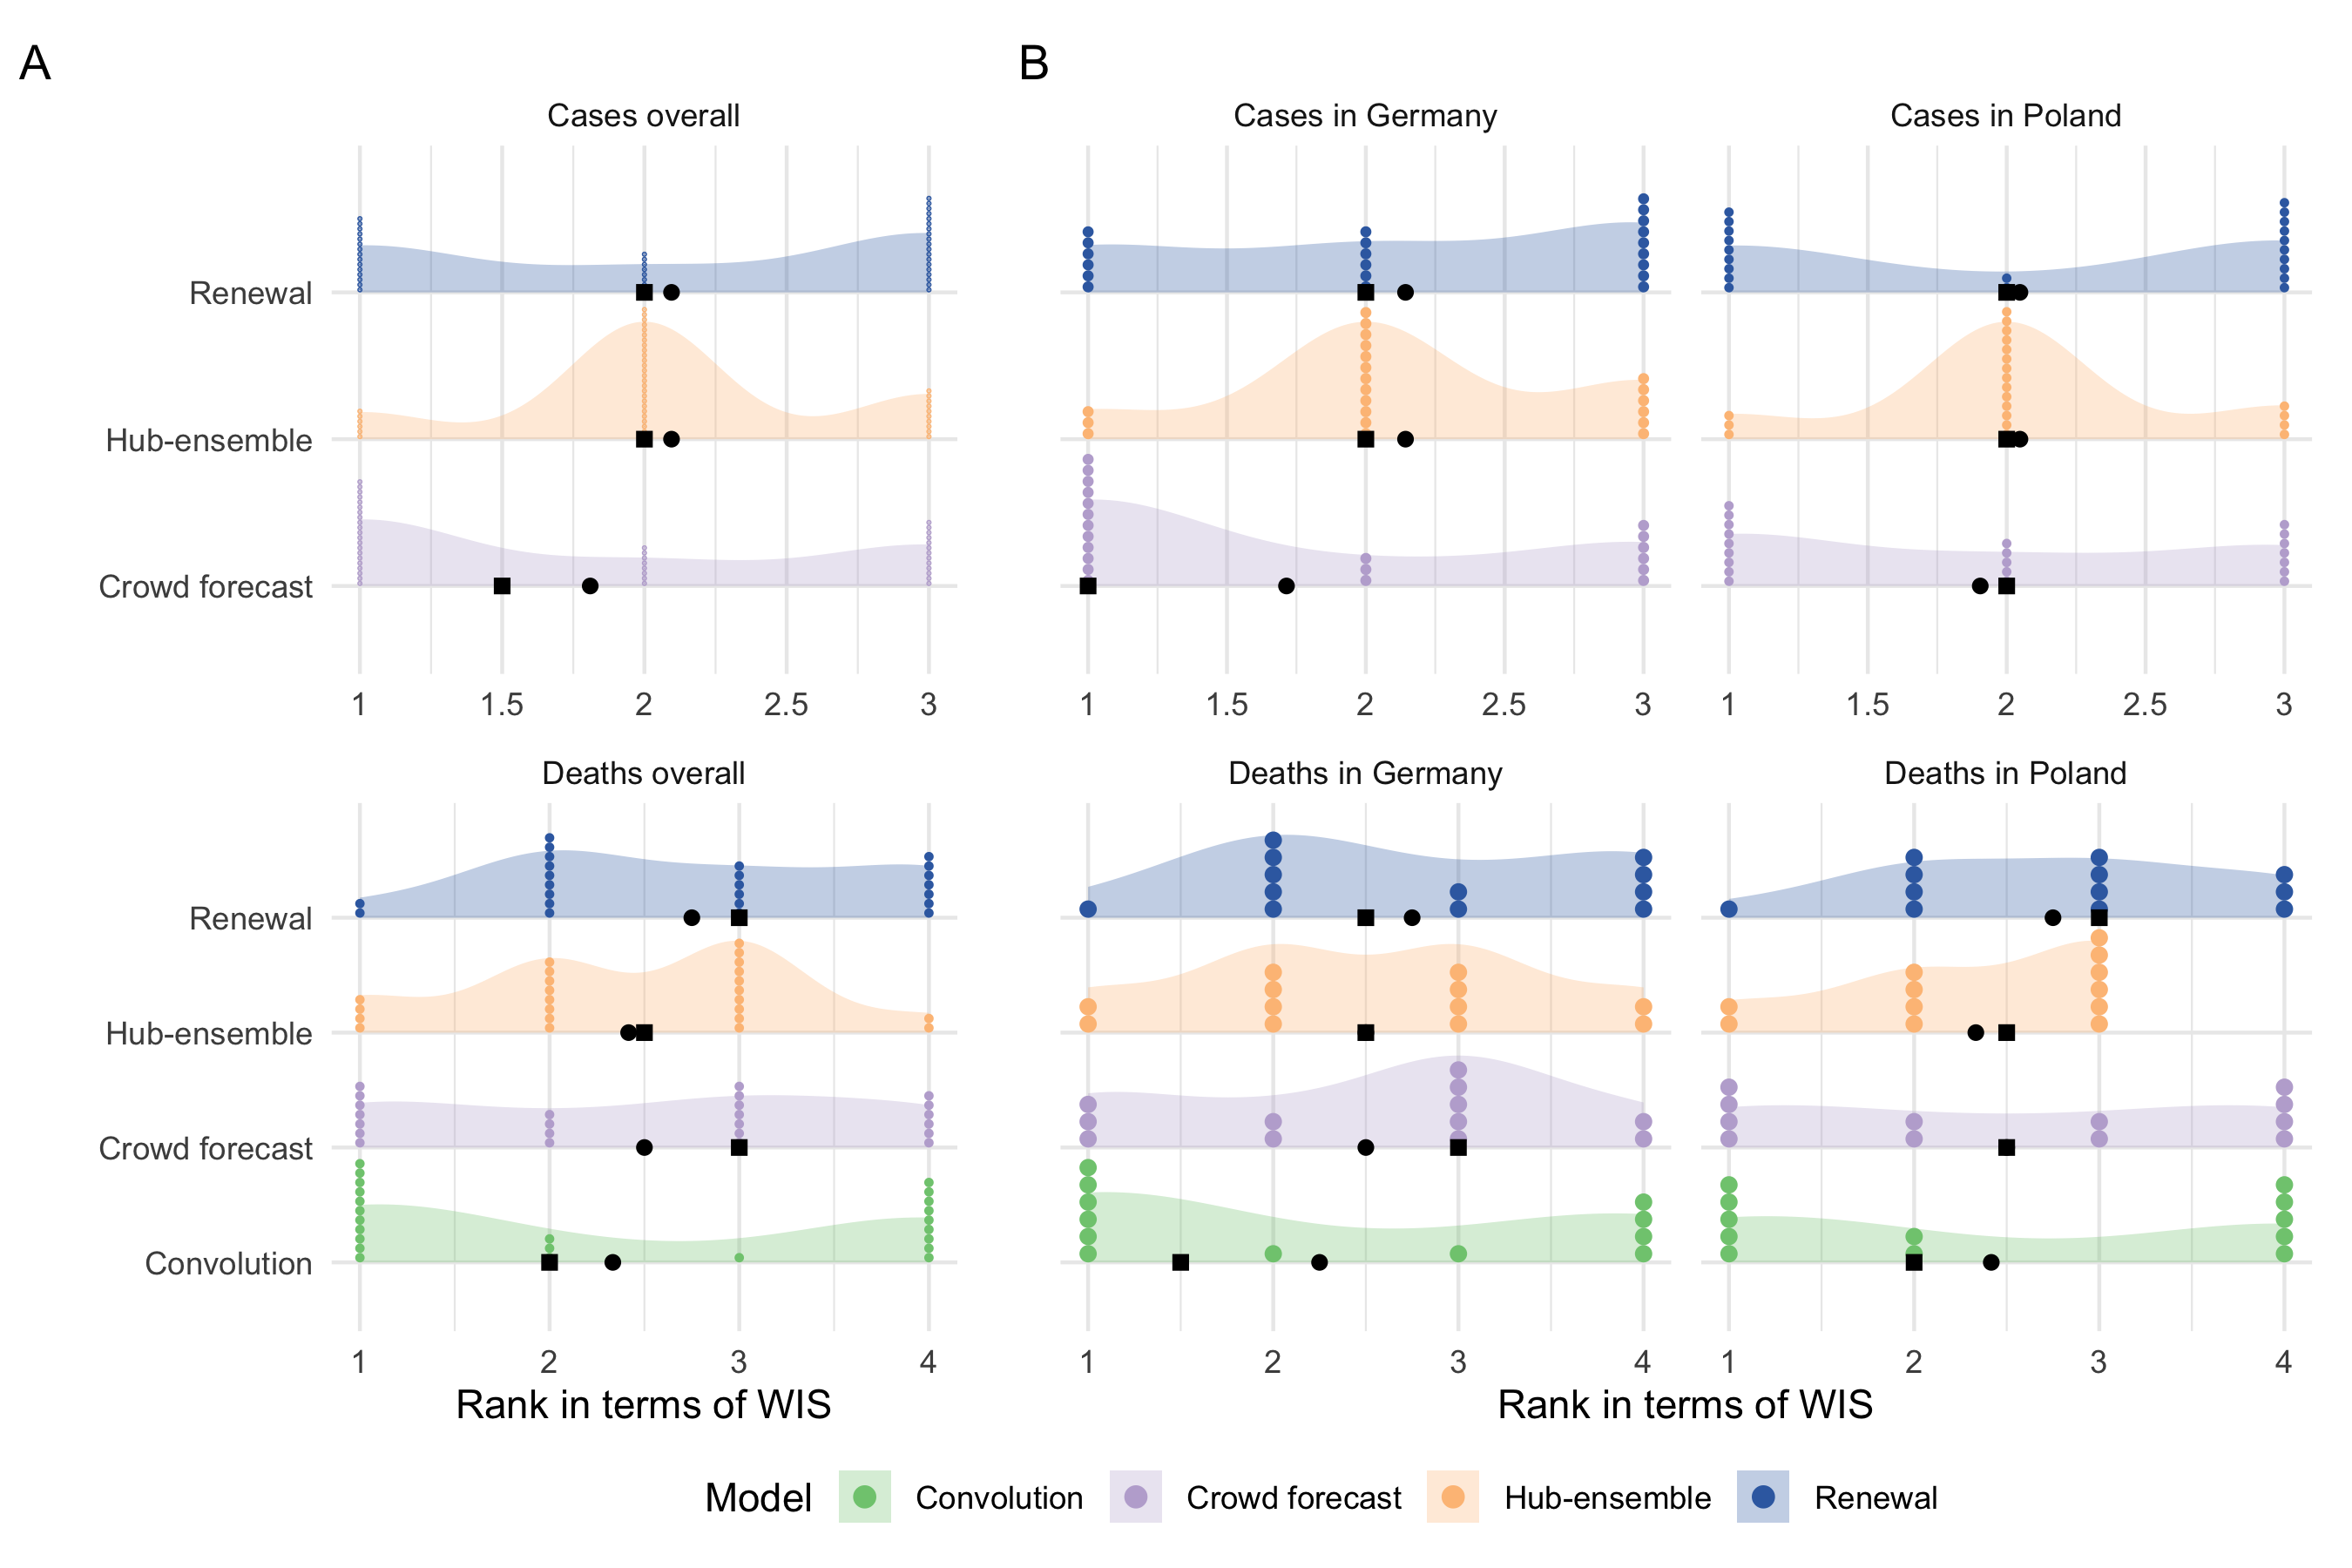
\includegraphics[width=1\linewidth,]{../../../analysis/plots/distribution_scores_wis-2-ranks} 
\caption{A: Distribution of the ranks (determined by the weighted interval score) for two week ahead forecasts of the different models and forecast targets. B: Distribution of ranks separate by country.}\label{fig:distribution-scores-ranks-2}
\end{figure}

\begin{figure}[H]
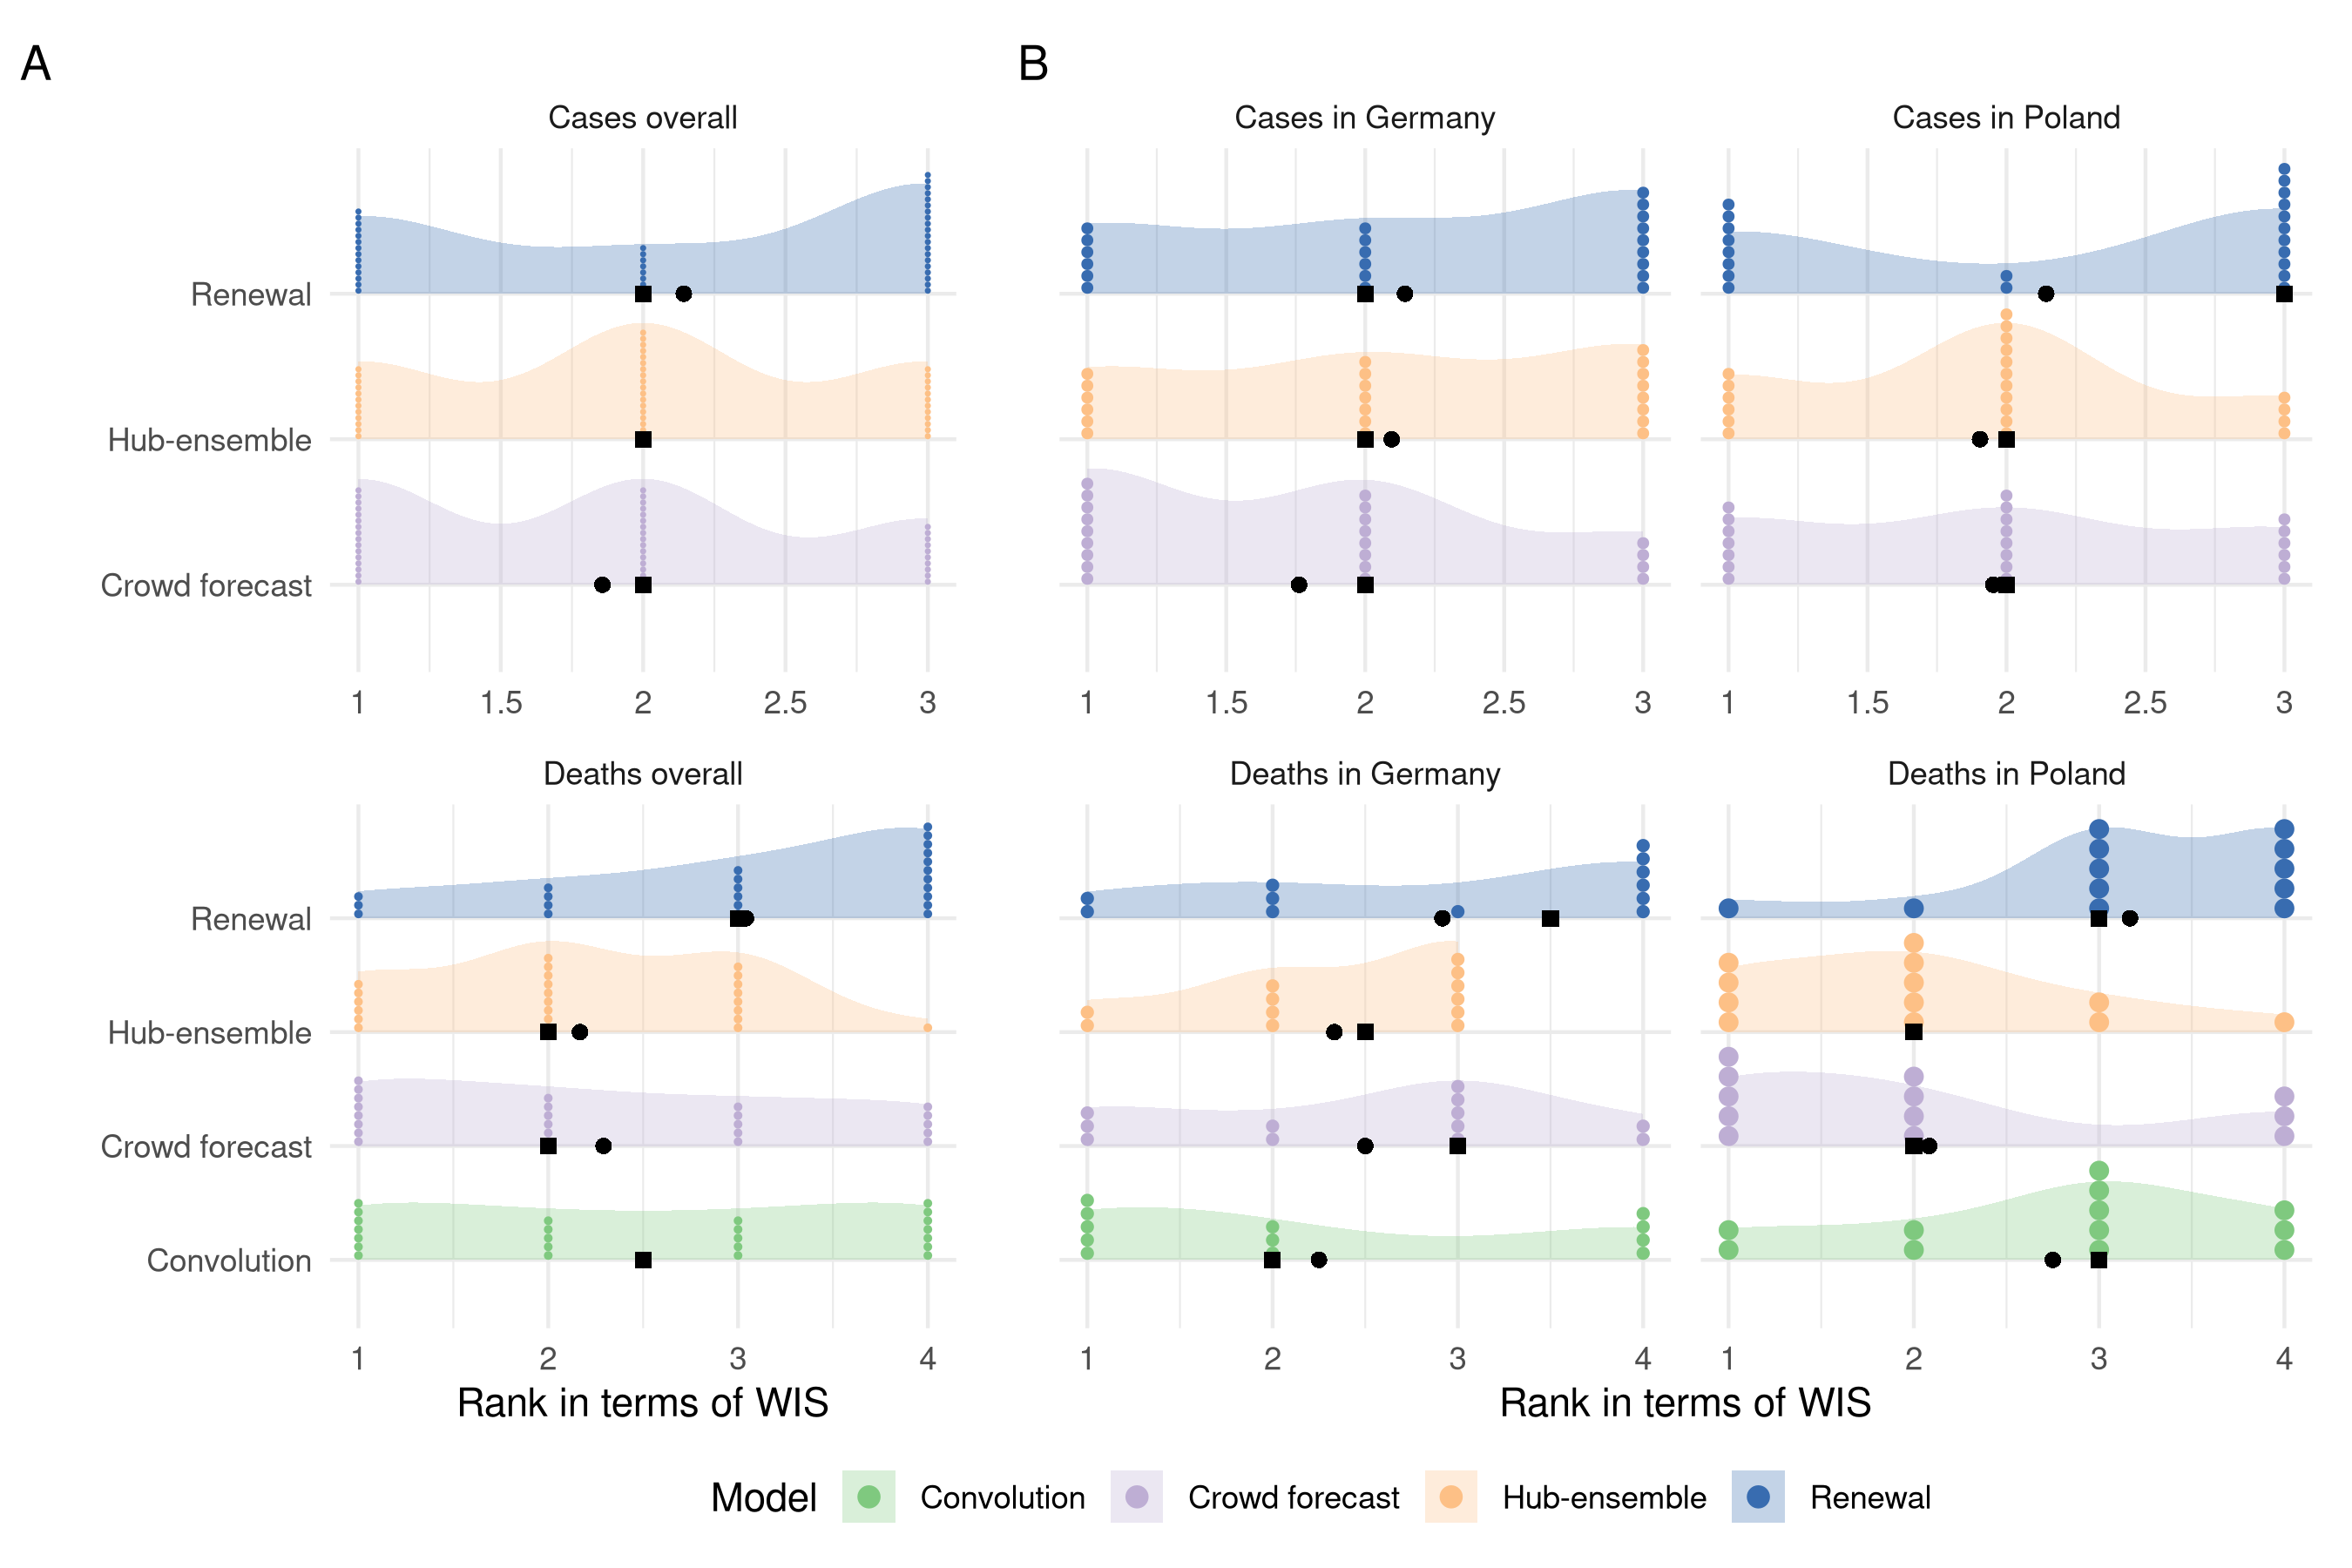
\includegraphics[width=1\linewidth,]{../../../analysis/plots/distribution_scores_wis-3-ranks} 
\caption{A: Distribution of the ranks (determined by the weighted interval score) for three week ahead forecasts of the different models and forecast targets. B: Distribution of ranks separate by country.}\label{fig:distribution-scores-ranks-3}
\end{figure}

\begin{figure}[H]
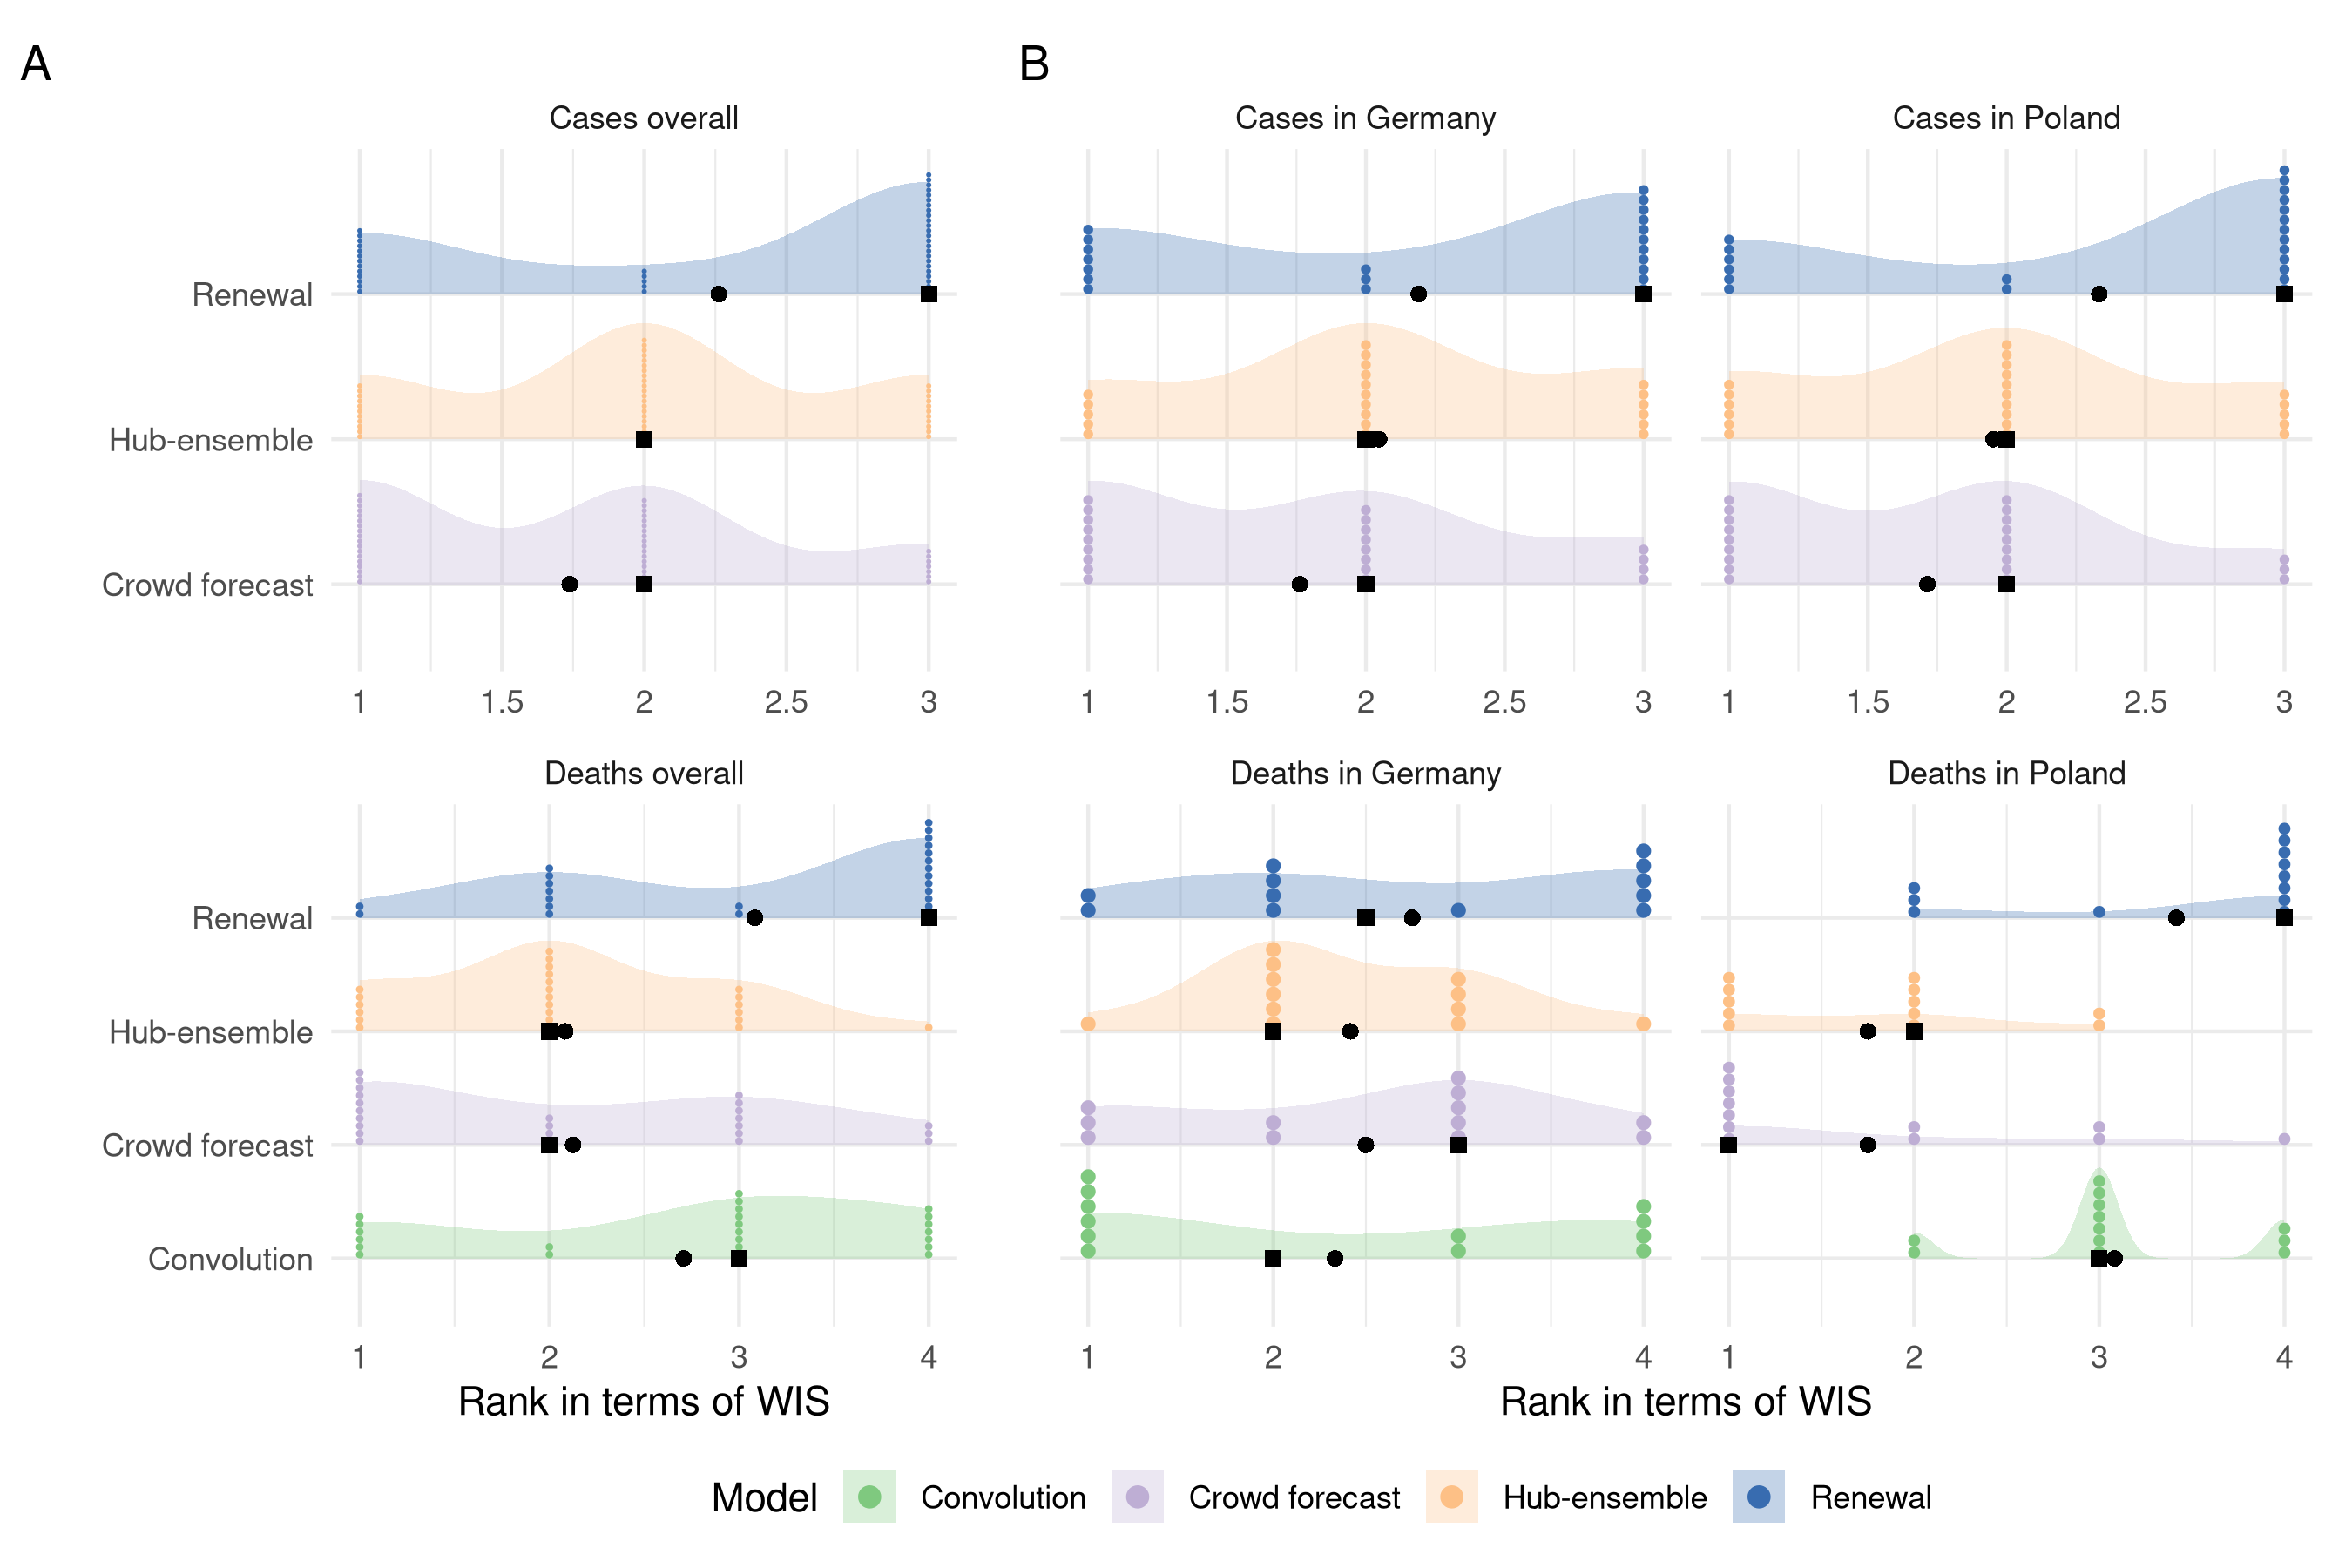
\includegraphics[width=1\linewidth,]{../../../analysis/plots/distribution_scores_wis-4-ranks} 
\caption{A: Distribution of the ranks (determined by the weighted interval score) for four week ahead forecasts of the different models and forecast targets. B: Distribution of ranks separate by country.}\label{fig:distribution-scores-ranks-4}
\end{figure}

\begin{figure}[H]
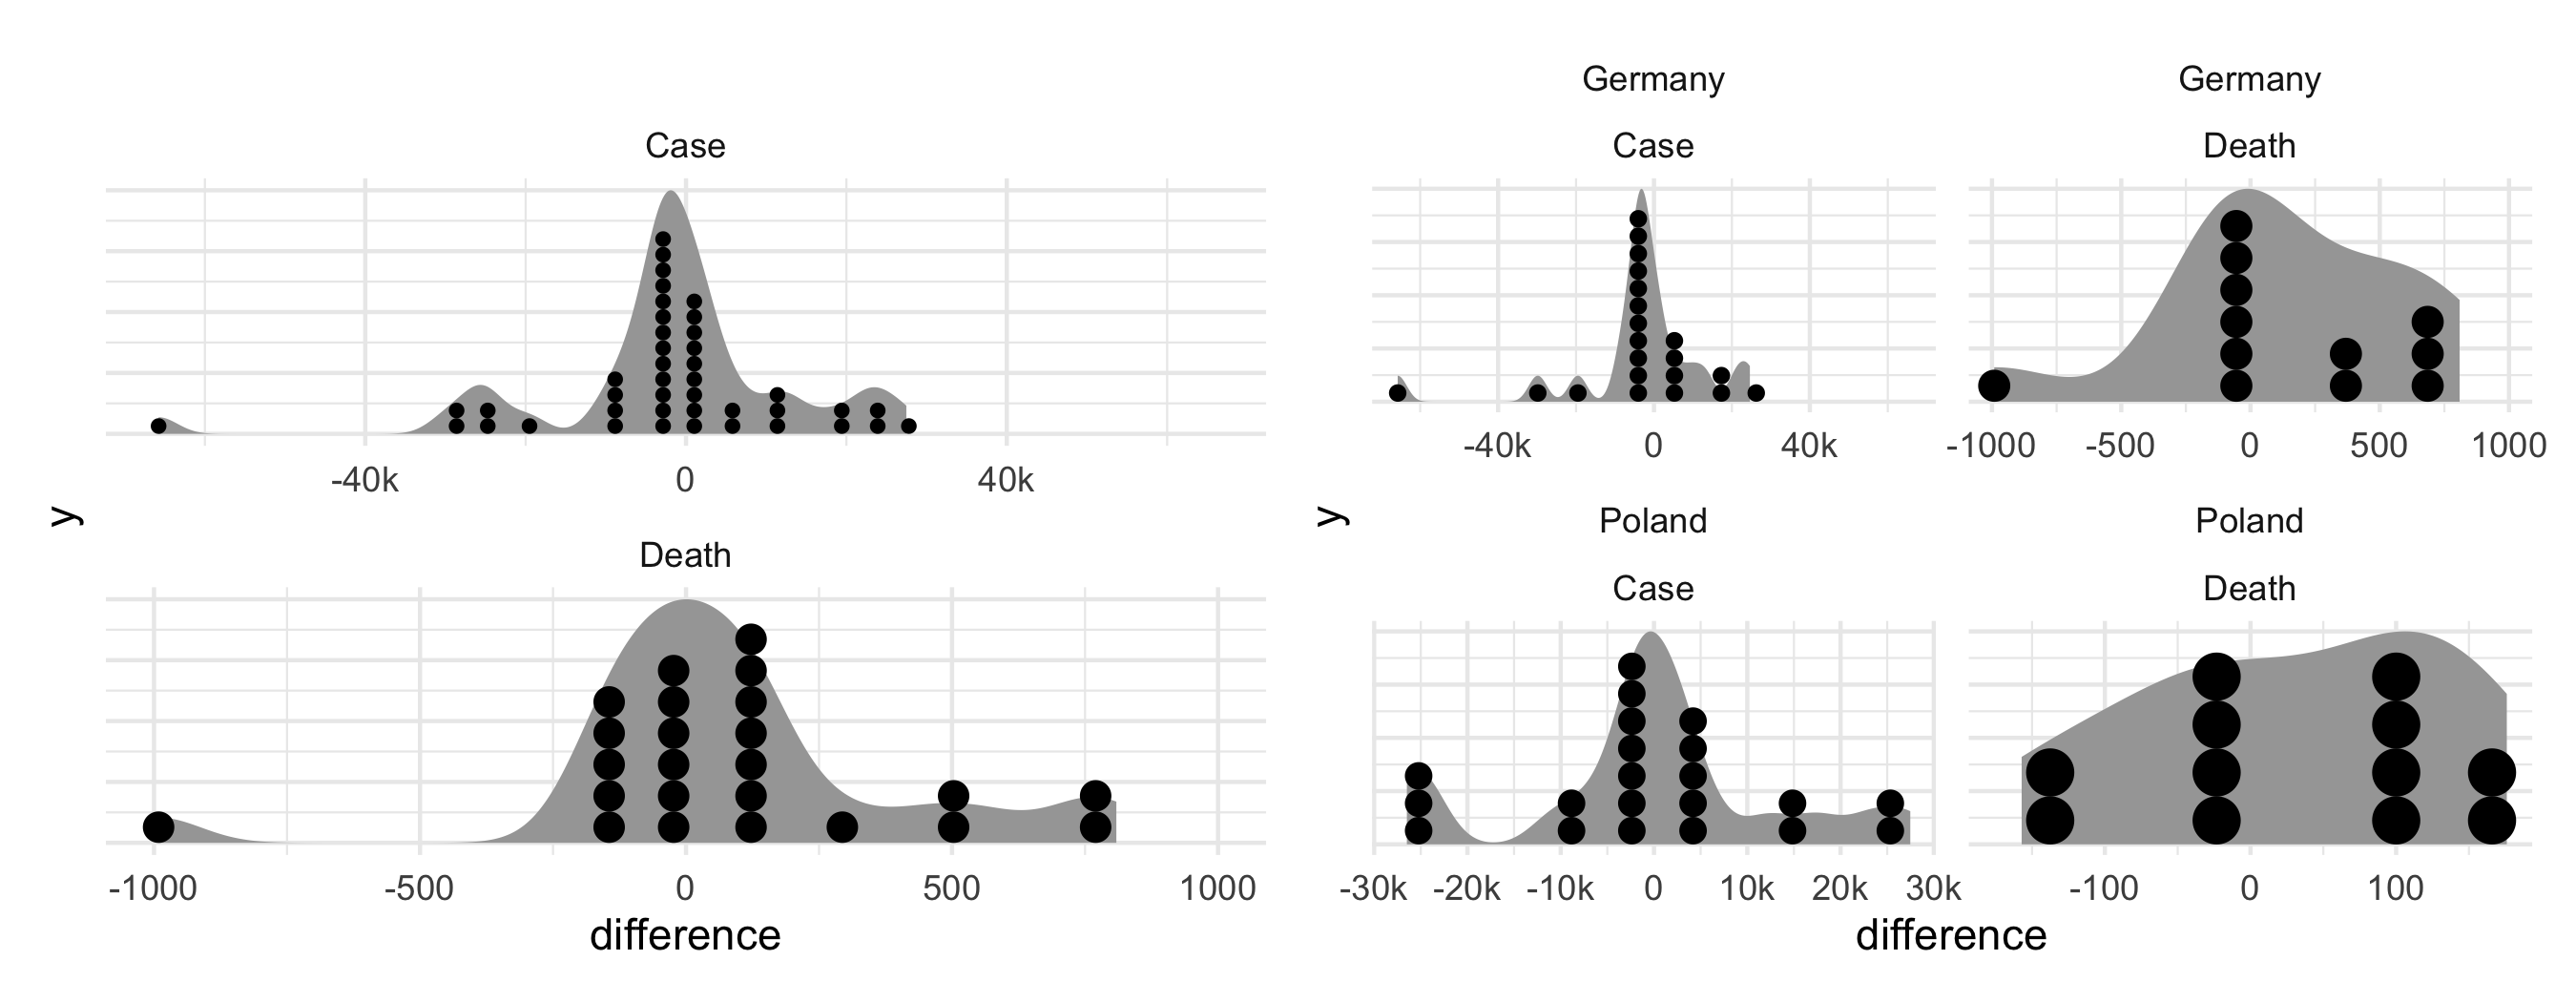
\includegraphics[width=1\linewidth,]{../../../analysis/plots/difference-wis-crowd-ensemble} 
\caption{Density plot with the difference in WIS between the Crowd forecast and the Hub ensemble (values below zero mean better performance of the Crowd forecasts) for a 2 week ahead forecast horizon.}\label{fig:distribution-scores-differences}
\end{figure}

\begin{figure}[H]
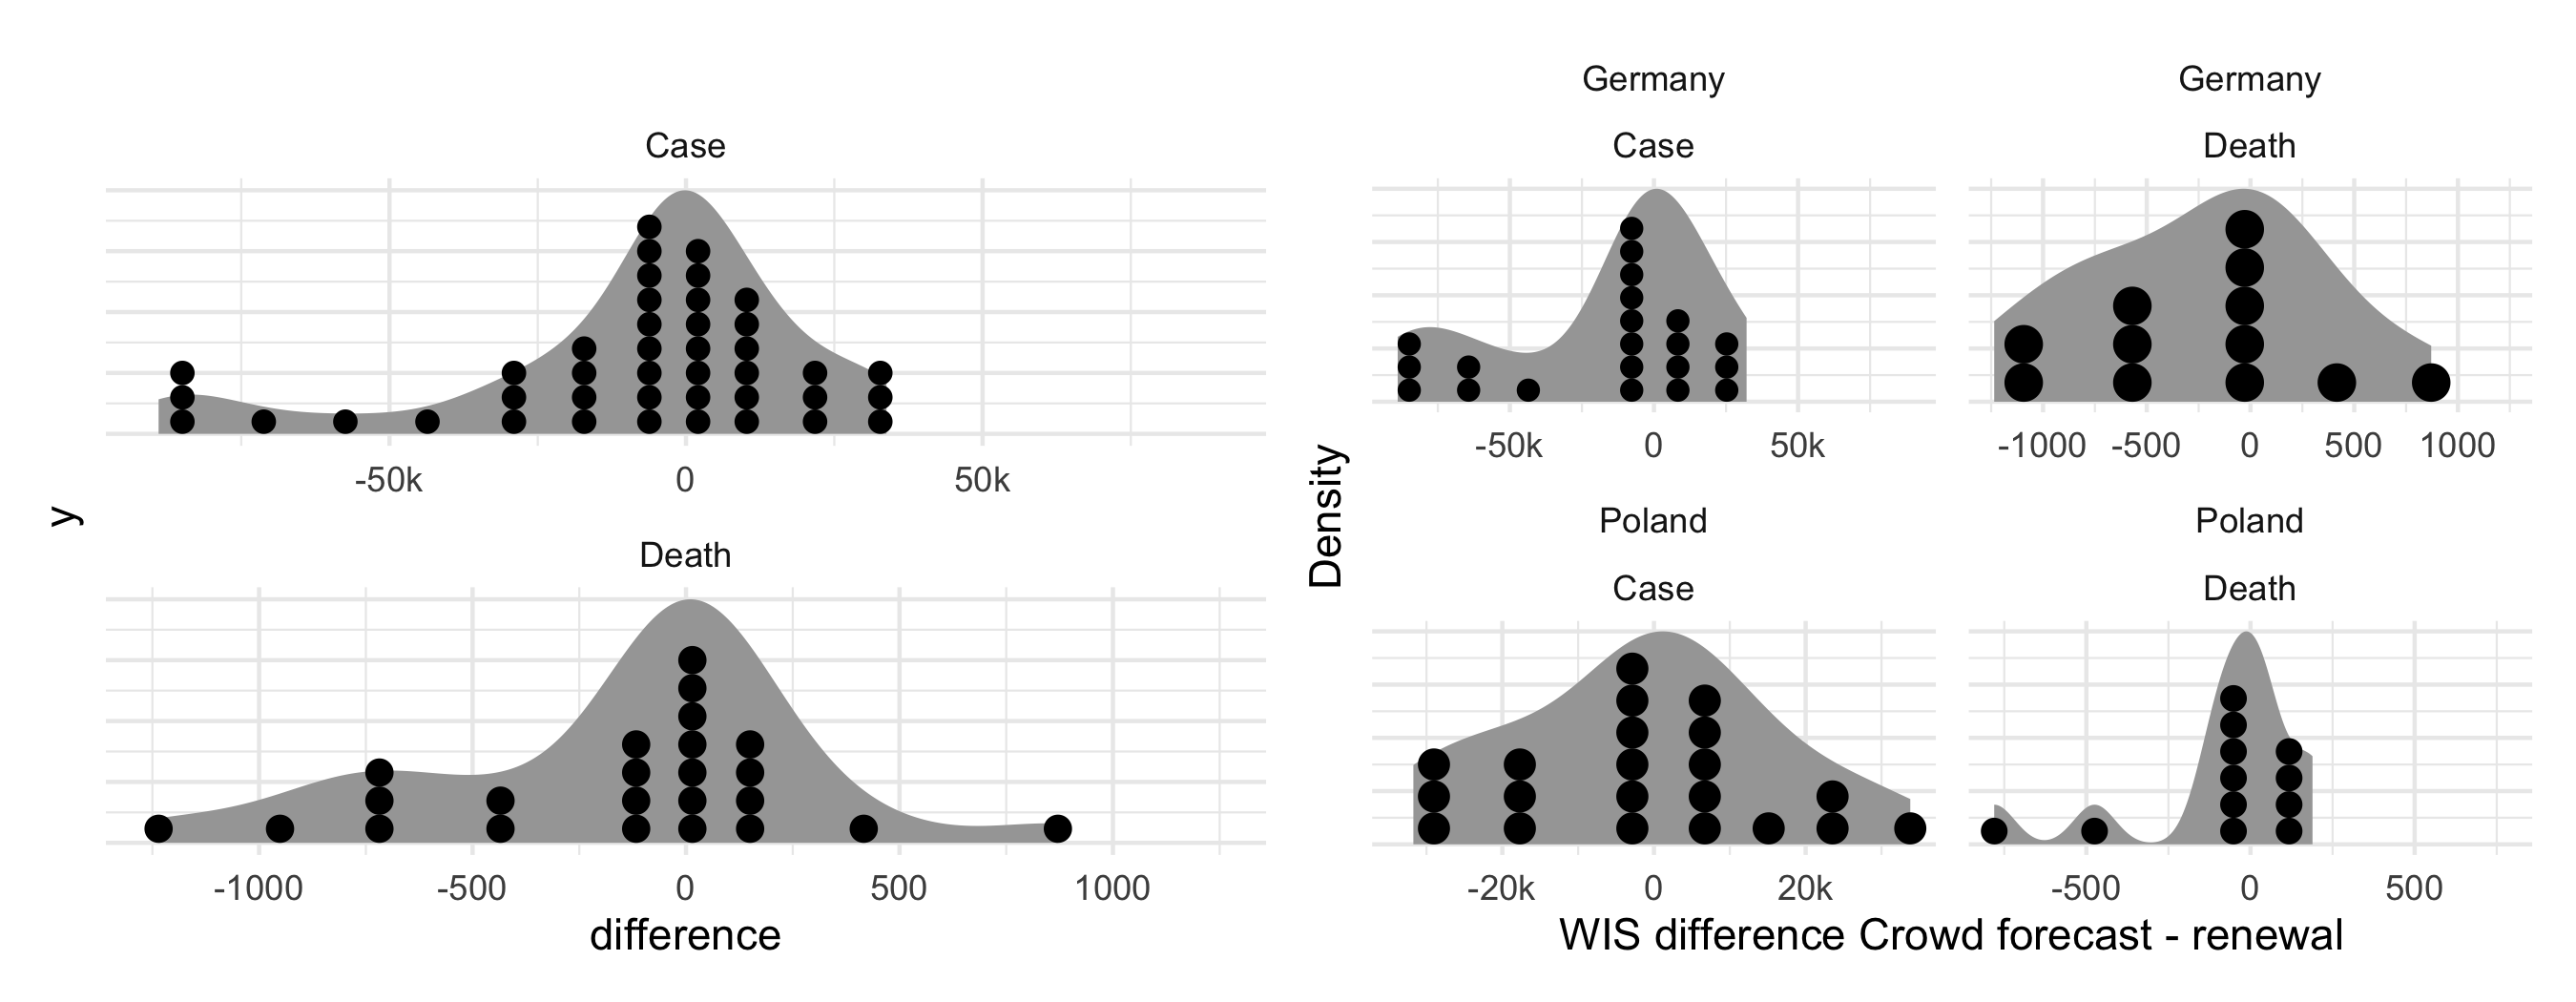
\includegraphics[width=1\linewidth,]{../../../analysis/plots/difference-wis-crowd-renewal} 
\caption{Density plot with the difference in WIS between the Crowd forecast and the Renewal model (values below zero mean better performance of the Crowd forecasts) for a 2 week ahead forecast horizon.}\label{fig:distribution-scores-differences-renewal}
\end{figure}

\newpage

\hypertarget{comparison-of-ensembles}{%
\subsection{Comparison of ensembles}\label{comparison-of-ensembles}}

\hypertarget{performance-visualisation-mean-ensemble}{%
\subsubsection{Performance visualisation mean
ensemble}\label{performance-visualisation-mean-ensemble}}

\begin{figure}[H]
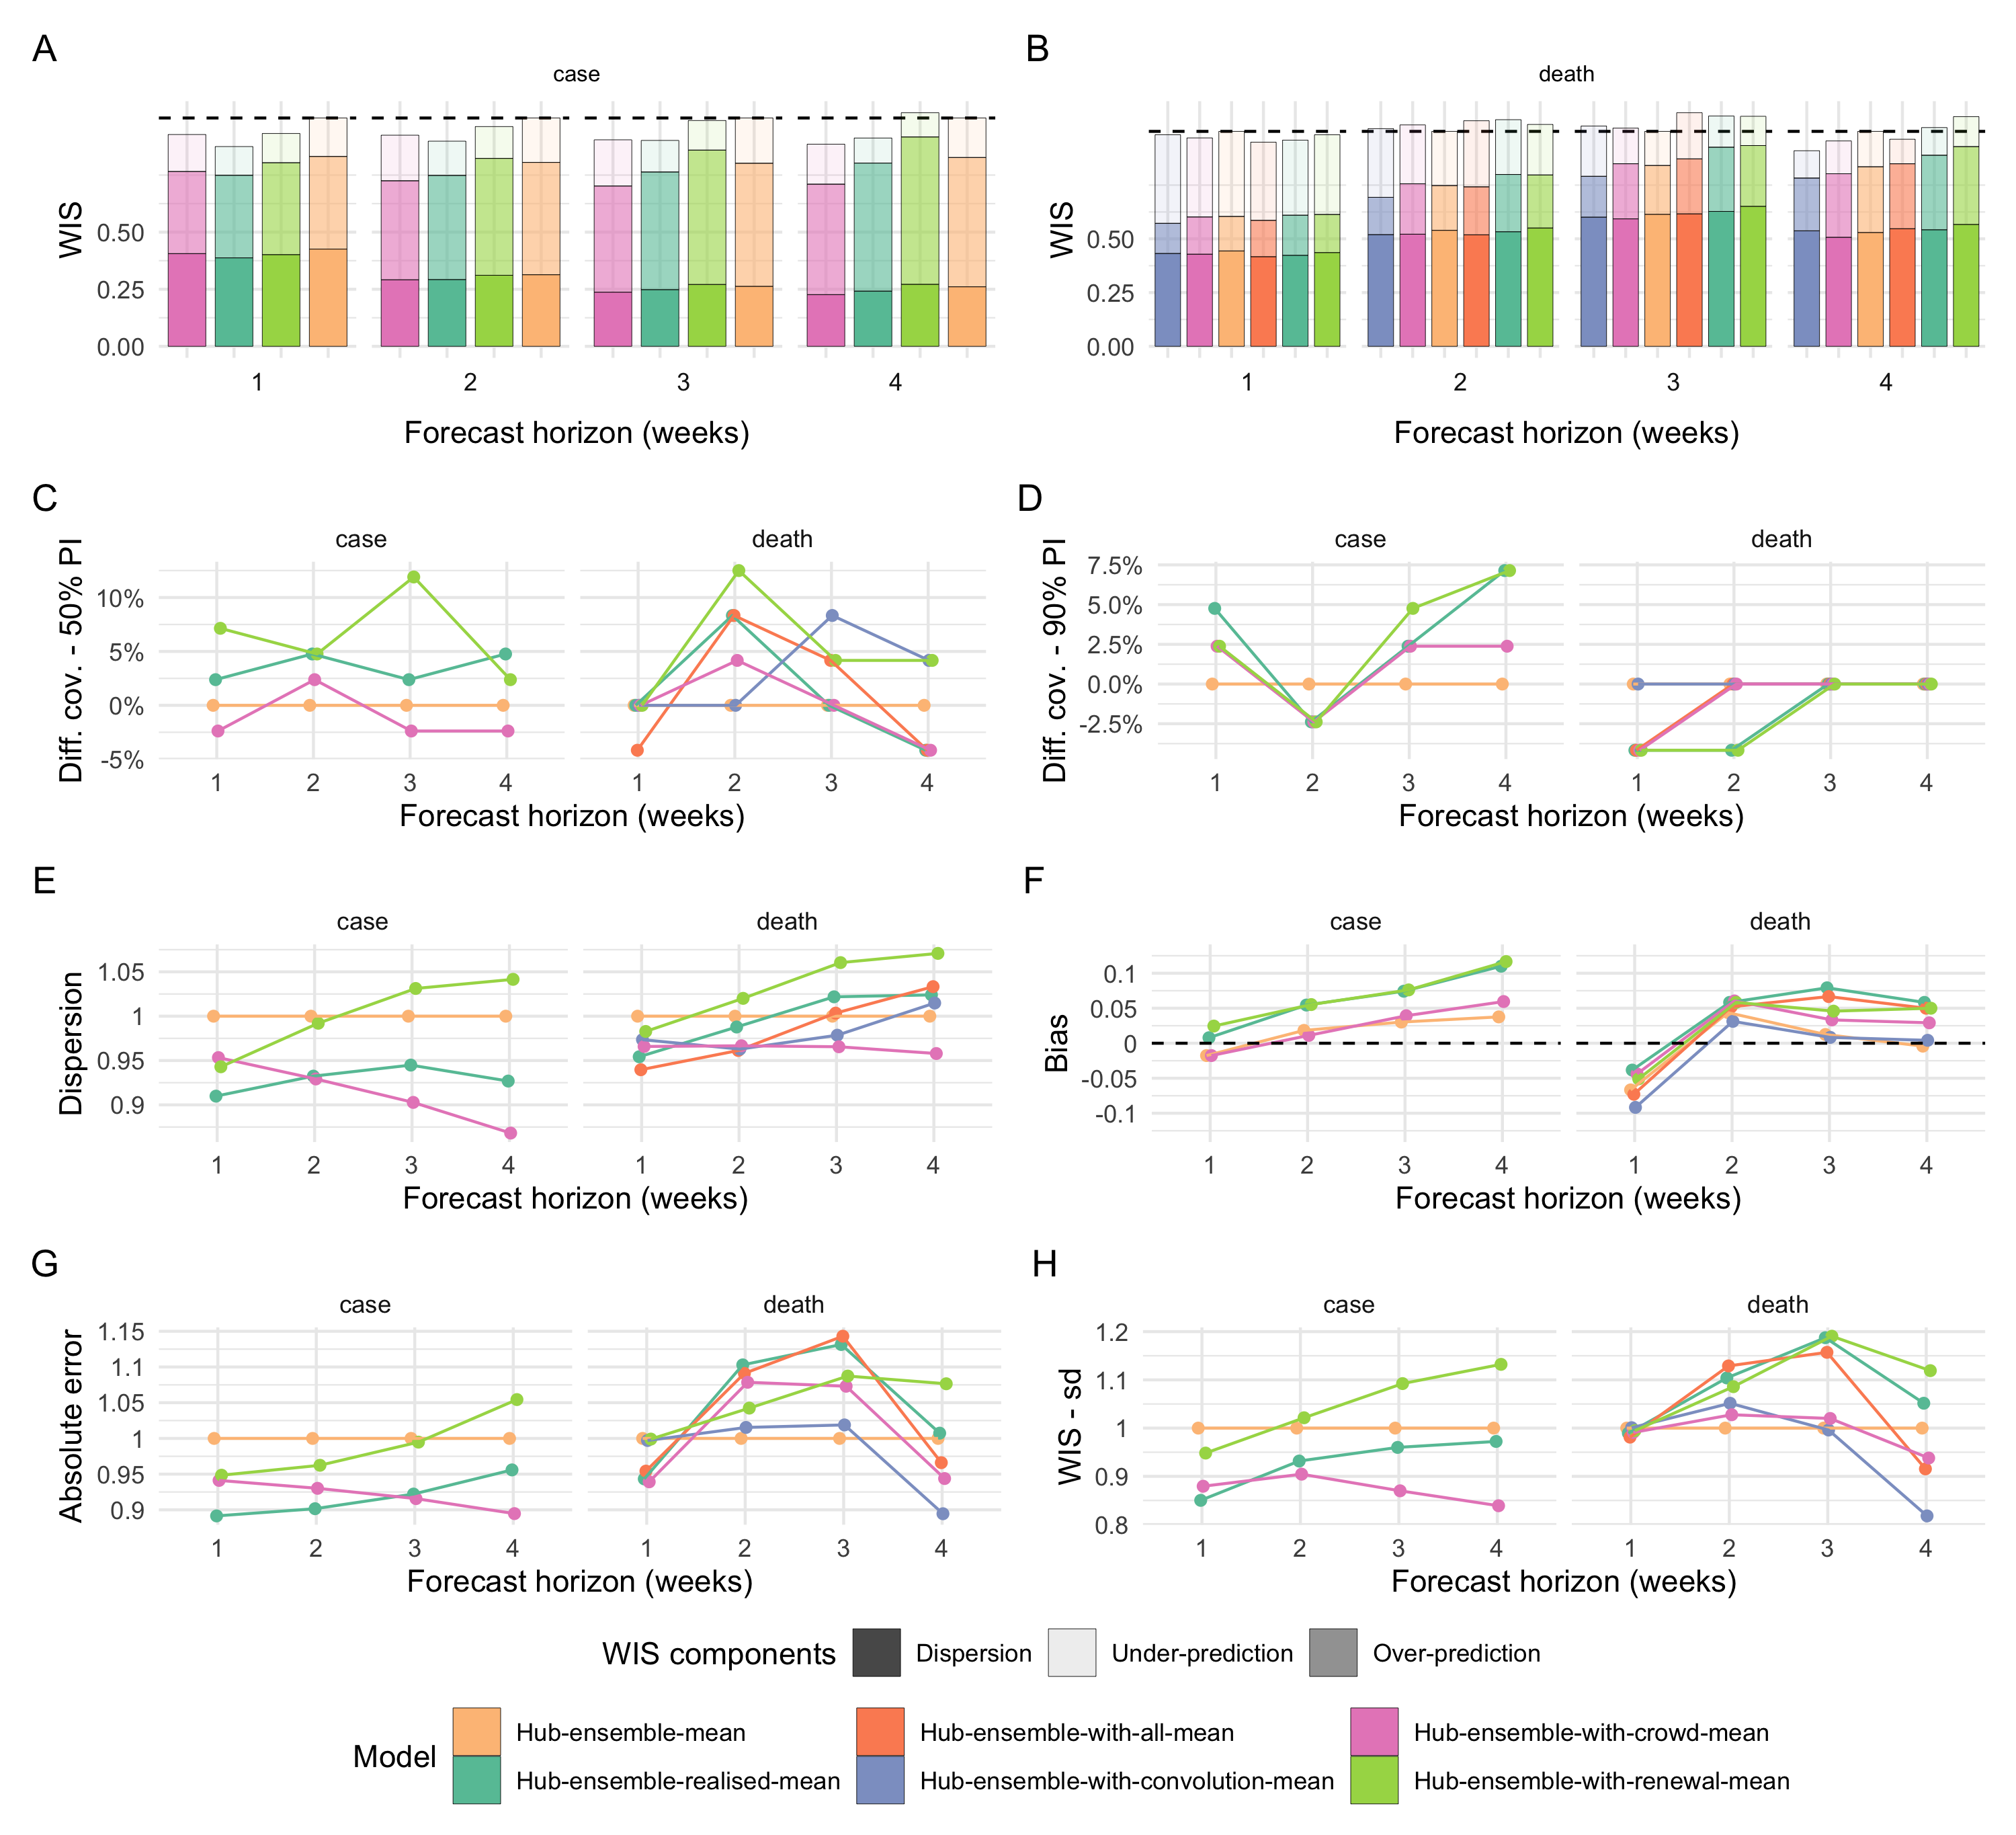
\includegraphics[width=1\linewidth,]{../../../analysis/plots/aggregate-performance-rel-ensemble-mean-v4}
\caption{Visualisation of aggregate performance metrics across forecast horizons for the different versions of the Hub mean ensemble. “Hub-ensemble”     extit{excludes} all our models, Hub-ensemble-all    extit{includes} all of our models, “Hub-ensemble-realised” is the actual hub-ensemble observed in reality, which includes the renewal model and the crowd forecasts, but ont the convolution model. Values (except for Bias) are computed as differences to the Hub ensemble which excludes our contributions. For Coverage, this is an absolute difference, for other metrics this is a percentage difference. A, B: mean weighted interval score (WIS) across horizons relative to the Hub ensemble (lower values indicate better performance). C, D: Empirical coverage of the 50\% and 90\% prediction intervals minus empirical coverage observed for the Hub ensemble. E: Dispersion relative to the dispersion of the Hub ensemble. Higher values mean greater dispersion of the forecast and imply ceteris paribus a worse score. F: Bias, i.e. general (relative) tendency to over- orunderpredict. Values are between -1 (complete under-prediction) and 1 (complete over-prediction) and 0 ideally. G: Absolute error of the median forecast relative to the Hub ensemble. H. Standard deviation of all WIS values for different horizons relative to the Hub ensemble.}\label{fig:agg-performance-ensemble-mean}
\end{figure}

\hypertarget{tables-median-ensemble}{%
\subsubsection{Tables median ensemble}\label{tables-median-ensemble}}

\begin{table}[!h]
\caption{\label{tab:score-table-ensemble-2}Scores for one and two week ahead forecasts (cut to three significant digits and rounded) for the different versions of the median ensemble. Note that scores for cases (which include the whole period from October 12th 2020 until March 1st 2021) and deaths (which include only forecasts from the 21st of December 2020 on) are computed on different subsets. Numbers in brackets show the metrics relative to the Hub ensemble (i.e. the median ensemble of all other models submitted to the German and Polish Forecast Hub, excluding our contributions). WIS is the mean weighted interval score (lower values are better), WIS - sd is the standard deviation of all scores achieved by a model. Dispersion, over-prediction and under-prediction together sum up to the weighted interval score. Bias (between -1 and 1, 0 is ideal) represents the general average tendency of a model to over- or underpredict. 50\% and 90\%-coverage are the percentage of observed values that fell within the 50\% and 90\% prediction intervals of a model.\\\hspace{\textwidth}}

\centering
\resizebox{\linewidth}{!}{
\begin{tabular}{>{}llccccccccc}
\toprule
  & Model & WIS & WIS - sd & dispersion & Underpred. & Overpred. & Bias & Abs. error & 50\%-Cov. & 90\%-Cov.\\
\midrule
\addlinespace[0.3em]
\multicolumn{11}{l}{\textbf{Cases}}\\
\hline
\cellcolor{white}{} & Hub-ensemble & 8770 (1) & 11700 (1) & 3670 (1) & 1230 (1) & 3870 (1) & -0.04 & 12700 (1) & 0.57 & 0.81\\
\cmidrule{2-11}
\cellcolor{white}{} & Hub-ensemble-realised & 6970 (0.79) & 8260 (0.71) & 3060 (0.83) & 943 (0.77) & 2970 (0.77) & 0.04 & 10800 (0.85) & 0.55 & 0.83\\
\cmidrule{2-11}
\cellcolor{white}{} & Hub-ensemble-with-crowd & 7820 (0.89) & 9630 (0.82) & 3270 (0.89) & 1210 (0.98) & 3330 (0.86) & -0.02 & 12000 (0.94) & 0.48 & 0.81\\
\cmidrule{2-11}
\cellcolor{white}{\multirow{-4}{*}{\raggedright\arraybackslash 1 wk ahead}} & Hub-ensemble-with-renewal & 7960 (0.91) & 10300 (0.88) & 3190 (0.87) & 1020 (0.83) & 3760 (0.97) & 0.04 & 12100 (0.95) & 0.57 & 0.83\\
\cmidrule{1-11}
\cellcolor{white}{} & Hub-ensemble & 18300 (1) & 21900 (1) & 6140 (1) & 3800 (1) & 8410 (1) & -0.03 & 26800 (1) & 0.43 & 0.64\\
\cmidrule{2-11}
\cellcolor{white}{} & Hub-ensemble-realised & 16400 (0.9) & 19600 (0.89) & 5350 (0.87) & 3290 (0.87) & 7730 (0.92) & 0.02 & 24200 (0.9) & 0.43 & 0.69\\
\cmidrule{2-11}
\cellcolor{white}{} & Hub-ensemble-with-crowd & 16900 (0.92) & 19600 (0.89) & 5230 (0.85) & 4310 (1.13) & 7370 (0.88) & 0.00 & 24600 (0.92) & 0.38 & 0.64\\
\cmidrule{2-11}
\cellcolor{white}{\multirow{-4}{*}{\raggedright\arraybackslash 2 wk ahead}} & Hub-ensemble-with-renewal & 17500 (0.96) & 21400 (0.98) & 5830 (0.95) & 2880 (0.76) & 8770 (1.04) & 0.00 & 25500 (0.95) & 0.45 & 0.71\\
\cmidrule{1-11}
\addlinespace[0.3em]
\multicolumn{11}{l}{\textbf{Deaths}}\\
\hline
\cellcolor{white}{} & Hub-ensemble & 248 (1) & 338 (1) & 92.2 (1) & 115 (1) & 41.6 (1) & -0.04 & 334 (1) & 0.62 & 0.92\\
\cmidrule{2-11}
\cellcolor{white}{} & Hub-ensemble-realised & 235 (0.95) & 332 (0.98) & 88.6 (0.96) & 90.4 (0.79) & 55.5 (1.33) & -0.01 & 323 (0.97) & 0.62 & 0.88\\
\cmidrule{2-11}
\cellcolor{white}{} & Hub-ensemble-with-all & 234 (0.94) & 331 (0.98) & 85.2 (0.92) & 98.1 (0.85) & 50.2 (1.21) & -0.05 & 329 (0.99) & 0.62 & 0.92\\
\cmidrule{2-11}
\cellcolor{white}{} & Hub-ensemble-with-convolution & 234 (0.94) & 329 (0.97) & 90.7 (0.98) & 118 (1.03) & 25.3 (0.61) & -0.08 & 333 (1) & 0.62 & 0.92\\
\cmidrule{2-11}
\cellcolor{white}{} & Hub-ensemble-with-crowd & 239 (0.96) & 337 (1) & 85.2 (0.92) & 99.6 (0.87) & 54.2 (1.3) & -0.03 & 322 (0.96) & 0.62 & 0.92\\
\cmidrule{2-11}
\cellcolor{white}{\multirow{-6}{*}{\raggedright\arraybackslash 1 wk ahead}} & Hub-ensemble-with-renewal & 246 (0.99) & 342 (1.01) & 91.5 (0.99) & 106 (0.92) & 48.6 (1.17) & -0.06 & 342 (1.02) & 0.67 & 0.92\\
\cmidrule{1-11}
\cellcolor{white}{} & Hub-ensemble & 292 (1) & 385 (1) & 132 (1) & 108 (1) & 51.9 (1) & 0.01 & 429 (1) & 0.62 & 0.96\\
\cmidrule{2-11}
\cellcolor{white}{} & Hub-ensemble-realised & 296 (1.01) & 398 (1.03) & 125 (0.95) & 91 (0.84) & 80.2 (1.55) & 0.05 & 486 (1.13) & 0.58 & 0.92\\
\cmidrule{2-11}
\cellcolor{white}{} & Hub-ensemble-with-all & 303 (1.04) & 423 (1.1) & 115 (0.87) & 122 (1.13) & 66.1 (1.27) & 0.00 & 483 (1.13) & 0.62 & 0.88\\
\cmidrule{2-11}
\cellcolor{white}{} & Hub-ensemble-with-convolution & 270 (0.92) & 385 (1) & 121 (0.92) & 119 (1.1) & 29.9 (0.58) & -0.04 & 403 (0.94) & 0.58 & 0.96\\
\cmidrule{2-11}
\cellcolor{white}{} & Hub-ensemble-with-crowd & 303 (1.04) & 392 (1.02) & 122 (0.92) & 106 (0.98) & 74.6 (1.44) & 0.03 & 499 (1.16) & 0.58 & 0.92\\
\cmidrule{2-11}
\cellcolor{white}{\multirow{-6}{*}{\raggedright\arraybackslash 2 wk ahead}} & Hub-ensemble-with-renewal & 296 (1.01) & 397 (1.03) & 128 (0.97) & 97.1 (0.9) & 71.2 (1.37) & -0.01 & 462 (1.08) & 0.67 & 0.92\\
\bottomrule
\end{tabular}}
\end{table}

\begin{table}[!h]
\caption{\label{tab:score-table-ensemble-4}Scores for three and four week ahead forecasts (cut to three significant digits and rounded) for the different versions of the median ensemble. Note that scores for cases (which include the whole period from October 12th 2020 until March 1st 2021) and deaths (which include only forecasts from the 21st of December 2020 on) are computed on different subsets. Numbers in brackets show the metrics relative to the Hub ensemble (i.e. the median ensemble of all other models submitted to the German and Polish Forecast Hub, excluding our contributions). WIS is the mean weighted interval score (lower values are better), WIS - sd is the standard deviation of all scores achieved by a model. Dispersion, over-prediction and under-prediction together sum up to the weighted interval score. Bias (between -1 and 1, 0 is ideal) represents the general average tendency of a model to over- or underpredict. 50\% and 90\%-coverage are the percentage of observed values that fell within the 50\% and 90\% prediction intervals of a model.\\\hspace{\textwidth}}

\centering
\resizebox{\linewidth}{!}{
\begin{tabular}{>{}llccccccccc}
\toprule
  & Model & WIS & WIS - sd & dispersion & Underpred. & Overpred. & Bias & Abs. error & 50\%-Cov. & 90\%-Cov.\\
\midrule
\addlinespace[0.3em]
\multicolumn{11}{l}{\textbf{Cases}}\\
\hline
\cellcolor{white}{} & Hub-ensemble & 33400 (1) & 40700 (1) & 9130 (1) & 7690 (1) & 16600 (1) & -0.01 & 46900 (1) & 0.29 & 0.62\\
\cmidrule{2-11}
\cellcolor{white}{} & Hub-ensemble-realised & 30800 (0.92) & 38600 (0.95) & 7910 (0.87) & 6890 (0.9) & 16000 (0.96) & 0.03 & 44200 (0.94) & 0.29 & 0.62\\
\cmidrule{2-11}
\cellcolor{white}{} & Hub-ensemble-with-crowd & 30800 (0.92) & 34100 (0.84) & 7500 (0.82) & 8960 (1.17) & 14300 (0.86) & 0.02 & 44100 (0.94) & 0.24 & 0.55\\
\cmidrule{2-11}
\cellcolor{white}{\multirow{-4}{*}{\raggedright\arraybackslash 3 wk ahead}} & Hub-ensemble-with-renewal & 34000 (1.02) & 43100 (1.06) & 8860 (0.97) & 6300 (0.82) & 18900 (1.14) & 0.02 & 48100 (1.03) & 0.29 & 0.60\\
\cmidrule{1-11}
\cellcolor{white}{} & Hub-ensemble & 55900 (1) & 73700 (1) & 12200 (1) & 12400 (1) & 31300 (1) & 0.01 & 74400 (1) & 0.24 & 0.52\\
\cmidrule{2-11}
\cellcolor{white}{} & Hub-ensemble-realised & 51200 (0.92) & 69900 (0.95) & 10900 (0.89) & 11100 (0.9) & 29300 (0.94) & 0.04 & 69600 (0.94) & 0.19 & 0.57\\
\cmidrule{2-11}
\cellcolor{white}{} & Hub-ensemble-with-crowd & 48800 (0.87) & 58600 (0.8) & 9700 (0.8) & 13700 (1.1) & 25400 (0.81) & 0.00 & 65800 (0.88) & 0.19 & 0.48\\
\cmidrule{2-11}
\cellcolor{white}{\multirow{-4}{*}{\raggedright\arraybackslash 4 wk ahead}} & Hub-ensemble-with-renewal & 59100 (1.06) & 84100 (1.14) & 12600 (1.03) & 10100 (0.81) & 36400 (1.16) & 0.01 & 78900 (1.06) & 0.29 & 0.55\\
\cmidrule{1-11}
\addlinespace[0.3em]
\multicolumn{11}{l}{\textbf{Deaths}}\\
\hline
\cellcolor{white}{} & Hub-ensemble & 319 (1) & 328 (1) & 172 (1) & 92.7 (1) & 55.1 (1) & -0.03 & 488 (1) & 0.54 & 0.96\\
\cmidrule{2-11}
\cellcolor{white}{} & Hub-ensemble-realised & 332 (1.04) & 388 (1.18) & 158 (0.92) & 78.7 (0.85) & 95 (1.72) & -0.02 & 547 (1.12) & 0.46 & 1.00\\
\cmidrule{2-11}
\cellcolor{white}{} & Hub-ensemble-with-all & 321 (1.01) & 385 (1.17) & 153 (0.89) & 100 (1.08) & 68.1 (1.24) & -0.01 & 535 (1.1) & 0.54 & 1.00\\
\cmidrule{2-11}
\cellcolor{white}{} & Hub-ensemble-with-convolution & 298 (0.93) & 337 (1.03) & 155 (0.9) & 106 (1.14) & 37.5 (0.68) & -0.04 & 441 (0.9) & 0.67 & 0.92\\
\cmidrule{2-11}
\cellcolor{white}{} & Hub-ensemble-with-crowd & 319 (1) & 342 (1.04) & 160 (0.93) & 85.1 (0.92) & 73.6 (1.34) & -0.02 & 547 (1.12) & 0.54 & 0.96\\
\cmidrule{2-11}
\cellcolor{white}{\multirow{-6}{*}{\raggedright\arraybackslash 3 wk ahead}} & Hub-ensemble-with-renewal & 332 (1.04) & 363 (1.11) & 168 (0.98) & 86.1 (0.93) & 78.2 (1.42) & -0.02 & 528 (1.08) & 0.58 & 0.96\\
\cmidrule{1-11}
\cellcolor{white}{} & Hub-ensemble & 424 (1) & 443 (1) & 212 (1) & 126 (1) & 85.7 (1) & -0.06 & 675 (1) & 0.58 & 0.92\\
\cmidrule{2-11}
\cellcolor{white}{} & Hub-ensemble-realised & 445 (1.05) & 532 (1.2) & 193 (0.91) & 107 (0.85) & 144 (1.68) & -0.03 & 700 (1.04) & 0.54 & 0.92\\
\cmidrule{2-11}
\cellcolor{white}{} & Hub-ensemble-with-all & 399 (0.94) & 438 (0.99) & 195 (0.92) & 105 (0.83) & 97.9 (1.14) & -0.05 & 692 (1.03) & 0.46 & 1.00\\
\cmidrule{2-11}
\cellcolor{white}{} & Hub-ensemble-with-convolution & 384 (0.91) & 387 (0.87) & 196 (0.92) & 122 (0.97) & 65.9 (0.77) & -0.06 & 602 (0.89) & 0.54 & 0.96\\
\cmidrule{2-11}
\cellcolor{white}{} & Hub-ensemble-with-crowd & 407 (0.96) & 456 (1.03) & 202 (0.95) & 105 (0.83) & 101 (1.18) & -0.03 & 669 (0.99) & 0.67 & 0.96\\
\cmidrule{2-11}
\cellcolor{white}{\multirow{-6}{*}{\raggedright\arraybackslash 4 wk ahead}} & Hub-ensemble-with-renewal & 457 (1.08) & 527 (1.19) & 208 (0.98) & 129 (1.02) & 121 (1.41) & -0.06 & 744 (1.1) & 0.50 & 0.96\\
\bottomrule
\end{tabular}}
\end{table}

\hypertarget{tables-mean-ensemble}{%
\subsubsection{Tables mean ensemble}\label{tables-mean-ensemble}}

\begin{table}[!h]
\caption{\label{tab:score-table-ensemble-mean-2}Scores for one and two week ahead forecasts (cut to three significant digits and rounded) for the different versions of the mean ensemble. Note that scores for cases (which include the whole period from October 12th 2020 until March 1st 2021) and deaths (which include only forecasts from the 21st of December 2020 on) are computed on different subsets. Numbers in brackets show the metrics relative to the Hub mean ensemble (i.e. the mean ensemble of all other models submitted to the German and Polish Forecast Hub, excluding our contributions). WIS is the mean weighted interval score (lower values are better), WIS - sd is the standard deviation of all scores achieved by a model. Dispersion, over-prediction and under-prediction together sum up to the weighted interval score. Bias (between -1 and 1, 0 is ideal) represents the general average tendency of a model to over- or underpredict. 50\% and 90\%-coverage are the percentage of observed values that fell within the 50\% and 90\% prediction intervals of a model.\\\hspace{\textwidth}}

\centering
\resizebox{\linewidth}{!}{
\begin{tabular}{>{}llccccccccc}
\toprule
  & Model & WIS & WIS - sd & dispersion & Underpred. & Overpred. & Bias & Abs. error & 50\%-Cov. & 90\%-Cov.\\
\midrule
\addlinespace[0.3em]
\multicolumn{11}{l}{\textbf{Cases}}\\
\hline
\cellcolor{white}{} & Hub-ensemble-mean & 8680 (1) & 10300 (1) & 3700 (1) & 1460 (1) & 3520 (1) & -0.02 & 13400 (1) & 0.50 & 0.86\\
\cmidrule{2-11}
\cellcolor{white}{} & Hub-ensemble-realised-mean & 7600 (0.88) & 8770 (0.85) & 3360 (0.91) & 1090 (0.75) & 3140 (0.89) & 0.01 & 11900 (0.89) & 0.52 & 0.90\\
\cmidrule{2-11}
\cellcolor{white}{} & Hub-ensemble-with-crowd-mean & 8050 (0.93) & 9070 (0.88) & 3520 (0.95) & 1410 (0.97) & 3120 (0.89) & -0.02 & 12600 (0.94) & 0.48 & 0.88\\
\cmidrule{2-11}
\cellcolor{white}{\multirow{-4}{*}{\raggedright\arraybackslash 1 wk ahead}} & Hub-ensemble-with-renewal-mean & 8090 (0.93) & 9780 (0.95) & 3490 (0.94) & 1110 (0.76) & 3490 (0.99) & 0.02 & 12700 (0.95) & 0.57 & 0.88\\
\cmidrule{1-11}
\cellcolor{white}{} & Hub-ensemble-mean & 19000 (1) & 22100 (1) & 5960 (1) & 3690 (1) & 9340 (1) & 0.02 & 28800 (1) & 0.33 & 0.79\\
\cmidrule{2-11}
\cellcolor{white}{} & Hub-ensemble-realised-mean & 17100 (0.9) & 20600 (0.93) & 5550 (0.93) & 2850 (0.77) & 8660 (0.93) & 0.05 & 26000 (0.9) & 0.38 & 0.76\\
\cmidrule{2-11}
\cellcolor{white}{} & Hub-ensemble-with-crowd-mean & 17600 (0.93) & 20000 (0.9) & 5540 (0.93) & 3790 (1.03) & 8230 (0.88) & 0.01 & 26800 (0.93) & 0.36 & 0.76\\
\cmidrule{2-11}
\cellcolor{white}{\multirow{-4}{*}{\raggedright\arraybackslash 2 wk ahead}} & Hub-ensemble-with-renewal-mean & 18300 (0.96) & 22600 (1.02) & 5910 (0.99) & 2640 (0.72) & 9720 (1.04) & 0.06 & 27700 (0.96) & 0.38 & 0.76\\
\cmidrule{1-11}
\addlinespace[0.3em]
\multicolumn{11}{l}{\textbf{Deaths}}\\
\hline
\cellcolor{white}{} & Hub-ensemble-mean & 229 (1) & 292 (1) & 101 (1) & 90.4 (1) & 36.7 (1) & -0.07 & 315 (1) & 0.71 & 0.92\\
\cmidrule{2-11}
\cellcolor{white}{} & Hub-ensemble-realised-mean & 219 (0.96) & 289 (0.99) & 96.8 (0.96) & 79.8 (0.88) & 42.6 (1.16) & -0.04 & 297 (0.94) & 0.71 & 0.88\\
\cmidrule{2-11}
\cellcolor{white}{} & Hub-ensemble-with-all-mean & 217 (0.95) & 287 (0.98) & 95.3 (0.94) & 83.1 (0.92) & 38.7 (1.05) & -0.07 & 300 (0.95) & 0.67 & 0.88\\
\cmidrule{2-11}
\cellcolor{white}{} & Hub-ensemble-with-convolution-mean & 225 (0.98) & 292 (1) & 98.7 (0.98) & 94.2 (1.04) & 32 (0.87) & -0.09 & 314 (1) & 0.71 & 0.92\\
\cmidrule{2-11}
\cellcolor{white}{} & Hub-ensemble-with-crowd-mean & 222 (0.97) & 289 (0.99) & 98 (0.97) & 84.1 (0.93) & 39.6 (1.08) & -0.04 & 295 (0.94) & 0.71 & 0.88\\
\cmidrule{2-11}
\cellcolor{white}{\multirow{-6}{*}{\raggedright\arraybackslash 1 wk ahead}} & Hub-ensemble-with-renewal-mean & 225 (0.98) & 290 (0.99) & 99.7 (0.99) & 84.7 (0.94) & 40.5 (1.1) & -0.05 & 314 (1) & 0.71 & 0.88\\
\cmidrule{1-11}
\cellcolor{white}{} & Hub-ensemble-mean & 256 (1) & 306 (1) & 138 (1) & 64.5 (1) & 53.2 (1) & 0.04 & 374 (1) & 0.67 & 0.96\\
\cmidrule{2-11}
\cellcolor{white}{} & Hub-ensemble-realised-mean & 270 (1.05) & 338 (1.1) & 136 (0.99) & 65.2 (1.01) & 68.1 (1.28) & 0.06 & 413 (1.1) & 0.75 & 0.92\\
\cmidrule{2-11}
\cellcolor{white}{} & Hub-ensemble-with-all-mean & 268 (1.05) & 346 (1.13) & 133 (0.96) & 78.7 (1.22) & 57.1 (1.07) & 0.05 & 408 (1.09) & 0.75 & 0.96\\
\cmidrule{2-11}
\cellcolor{white}{} & Hub-ensemble-with-convolution-mean & 259 (1.01) & 322 (1.05) & 133 (0.96) & 81.7 (1.27) & 44.4 (0.83) & 0.03 & 380 (1.02) & 0.67 & 0.96\\
\cmidrule{2-11}
\cellcolor{white}{} & Hub-ensemble-with-crowd-mean & 264 (1.03) & 315 (1.03) & 133 (0.96) & 70.1 (1.09) & 60 (1.13) & 0.06 & 404 (1.08) & 0.71 & 0.96\\
\cmidrule{2-11}
\cellcolor{white}{\multirow{-6}{*}{\raggedright\arraybackslash 2 wk ahead}} & Hub-ensemble-with-renewal-mean & 264 (1.03) & 332 (1.08) & 141 (1.02) & 60.1 (0.93) & 63.1 (1.19) & 0.06 & 390 (1.04) & 0.79 & 0.92\\
\bottomrule
\end{tabular}}
\end{table}

\begin{table}[!h]
\caption{\label{tab:score-table-ensemble-mean-4}Scores for three and four week ahead forecasts (cut to three significant digits and rounded) for the different versions of the mean ensemble. Note that scores for cases (which include the whole period from October 12th 2020 until March 1st 2021) and deaths (which include only forecasts from the 21st of December 2020 on) are computed on different subsets. Numbers in brackets show the metrics relative to the Hub mean ensemble (i.e. the mean ensemble of all other models submitted to the German and Polish Forecast Hub, excluding our contributions). WIS is the mean weighted interval score (lower values are better), WIS - sd is the standard deviation of all scores achieved by a model. Dispersion, over-prediction and under-prediction together sum up to the weighted interval score. Bias (between -1 and 1, 0 is ideal) represents the general average tendency of a model to over- or underpredict. 50\% and 90\%-coverage are the percentage of observed values that fell within the 50\% and 90\% prediction intervals of a model.\\\hspace{\textwidth}}

\centering
\resizebox{\linewidth}{!}{
\begin{tabular}{>{}llccccccccc}
\toprule
  & Model & WIS & WIS - sd & dispersion & Underpred. & Overpred. & Bias & Abs. error & 50\%-Cov. & 90\%-Cov.\\
\midrule
\addlinespace[0.3em]
\multicolumn{11}{l}{\textbf{Cases}}\\
\hline
\cellcolor{white}{} & Hub-ensemble-mean & 35600 (1) & 42100 (1) & 9340 (1) & 7050 (1) & 19200 (1) & 0.03 & 51200 (1) & 0.26 & 0.62\\
\cmidrule{2-11}
\cellcolor{white}{} & Hub-ensemble-realised-mean & 32100 (0.9) & 40500 (0.96) & 8830 (0.95) & 4920 (0.7) & 18300 (0.95) & 0.07 & 47200 (0.92) & 0.29 & 0.64\\
\cmidrule{2-11}
\cellcolor{white}{} & Hub-ensemble-with-crowd-mean & 32200 (0.9) & 36700 (0.87) & 8430 (0.9) & 7190 (1.02) & 16500 (0.86) & 0.04 & 46900 (0.92) & 0.24 & 0.64\\
\cmidrule{2-11}
\cellcolor{white}{\multirow{-4}{*}{\raggedright\arraybackslash 3 wk ahead}} & Hub-ensemble-with-renewal-mean & 35200 (0.99) & 46000 (1.09) & 9630 (1.03) & 4600 (0.65) & 20900 (1.09) & 0.08 & 51000 (1) & 0.38 & 0.67\\
\cmidrule{1-11}
\cellcolor{white}{} & Hub-ensemble-mean & 60300 (1) & 79300 (1) & 15700 (1) & 10400 (1) & 34100 (1) & 0.04 & 78600 (1) & 0.29 & 0.57\\
\cmidrule{2-11}
\cellcolor{white}{} & Hub-ensemble-realised-mean & 55000 (0.91) & 77100 (0.97) & 14600 (0.93) & 6620 (0.64) & 33800 (0.99) & 0.11 & 75200 (0.96) & 0.33 & 0.64\\
\cmidrule{2-11}
\cellcolor{white}{} & Hub-ensemble-with-crowd-mean & 53400 (0.89) & 66600 (0.84) & 13700 (0.87) & 10600 (1.02) & 29200 (0.86) & 0.06 & 70400 (0.9) & 0.26 & 0.60\\
\cmidrule{2-11}
\cellcolor{white}{\multirow{-4}{*}{\raggedright\arraybackslash 4 wk ahead}} & Hub-ensemble-with-renewal-mean & 61700 (1.02) & 89800 (1.13) & 16400 (1.04) & 6400 (0.62) & 38900 (1.14) & 0.12 & 82900 (1.05) & 0.31 & 0.64\\
\cmidrule{1-11}
\addlinespace[0.3em]
\multicolumn{11}{l}{\textbf{Deaths}}\\
\hline
\cellcolor{white}{} & Hub-ensemble-mean & 289 (1) & 293 (1) & 178 (1) & 45.9 (1) & 65.7 (1) & 0.01 & 443 (1) & 0.58 & 1.00\\
\cmidrule{2-11}
\cellcolor{white}{} & Hub-ensemble-realised-mean & 310 (1.07) & 348 (1.19) & 182 (1.02) & 42 (0.92) & 86.5 (1.32) & 0.08 & 502 (1.13) & 0.58 & 1.00\\
\cmidrule{2-11}
\cellcolor{white}{} & Hub-ensemble-with-all-mean & 315 (1.09) & 339 (1.16) & 178 (1) & 62.2 (1.36) & 74 (1.13) & 0.07 & 507 (1.14) & 0.62 & 1.00\\
\cmidrule{2-11}
\cellcolor{white}{} & Hub-ensemble-with-convolution-mean & 297 (1.03) & 292 (1) & 174 (0.98) & 67.7 (1.47) & 55 (0.84) & 0.01 & 452 (1.02) & 0.67 & 1.00\\
\cmidrule{2-11}
\cellcolor{white}{} & Hub-ensemble-with-crowd-mean & 294 (1.02) & 299 (1.02) & 172 (0.97) & 48 (1.05) & 74.2 (1.13) & 0.03 & 476 (1.07) & 0.58 & 1.00\\
\cmidrule{2-11}
\cellcolor{white}{\multirow{-6}{*}{\raggedright\arraybackslash 3 wk ahead}} & Hub-ensemble-with-renewal-mean & 310 (1.07) & 349 (1.19) & 189 (1.06) & 39.4 (0.86) & 81.9 (1.25) & 0.05 & 482 (1.09) & 0.62 & 1.00\\
\cmidrule{1-11}
\cellcolor{white}{} & Hub-ensemble-mean & 437 (1) & 568 (1) & 232 (1) & 72 (1) & 134 (1) & 0.00 & 702 (1) & 0.62 & 1.00\\
\cmidrule{2-11}
\cellcolor{white}{} & Hub-ensemble-realised-mean & 445 (1.02) & 598 (1.05) & 237 (1.02) & 56.4 (0.78) & 152 (1.13) & 0.06 & 707 (1.01) & 0.58 & 1.00\\
\cmidrule{2-11}
\cellcolor{white}{} & Hub-ensemble-with-all-mean & 421 (0.96) & 520 (0.92) & 239 (1.03) & 49.9 (0.69) & 132 (0.99) & 0.05 & 678 (0.97) & 0.58 & 1.00\\
\cmidrule{2-11}
\cellcolor{white}{} & Hub-ensemble-with-convolution-mean & 398 (0.91) & 465 (0.82) & 235 (1.01) & 55.6 (0.77) & 107 (0.8) & 0.00 & 628 (0.89) & 0.67 & 1.00\\
\cmidrule{2-11}
\cellcolor{white}{} & Hub-ensemble-with-crowd-mean & 418 (0.96) & 533 (0.94) & 222 (0.96) & 66.8 (0.93) & 129 (0.96) & 0.03 & 662 (0.94) & 0.58 & 1.00\\
\cmidrule{2-11}
\cellcolor{white}{\multirow{-6}{*}{\raggedright\arraybackslash 4 wk ahead}} & Hub-ensemble-with-renewal-mean & 467 (1.07) & 636 (1.12) & 248 (1.07) & 61 (0.85) & 158 (1.18) & 0.05 & 755 (1.08) & 0.67 & 1.00\\
\bottomrule
\end{tabular}}
\end{table}

\clearpage

\hypertarget{sensitivity-analysis}{%
\subsection{Sensitivity analysis}\label{sensitivity-analysis}}

In the original analysis, cases and deaths were scored on different
periods, as the convolution model was only added later. This sensitivity
shows performance of all models restricted to the period from December
14 2020 until March 1st 2021 where all models were available.

\begin{figure}[H]
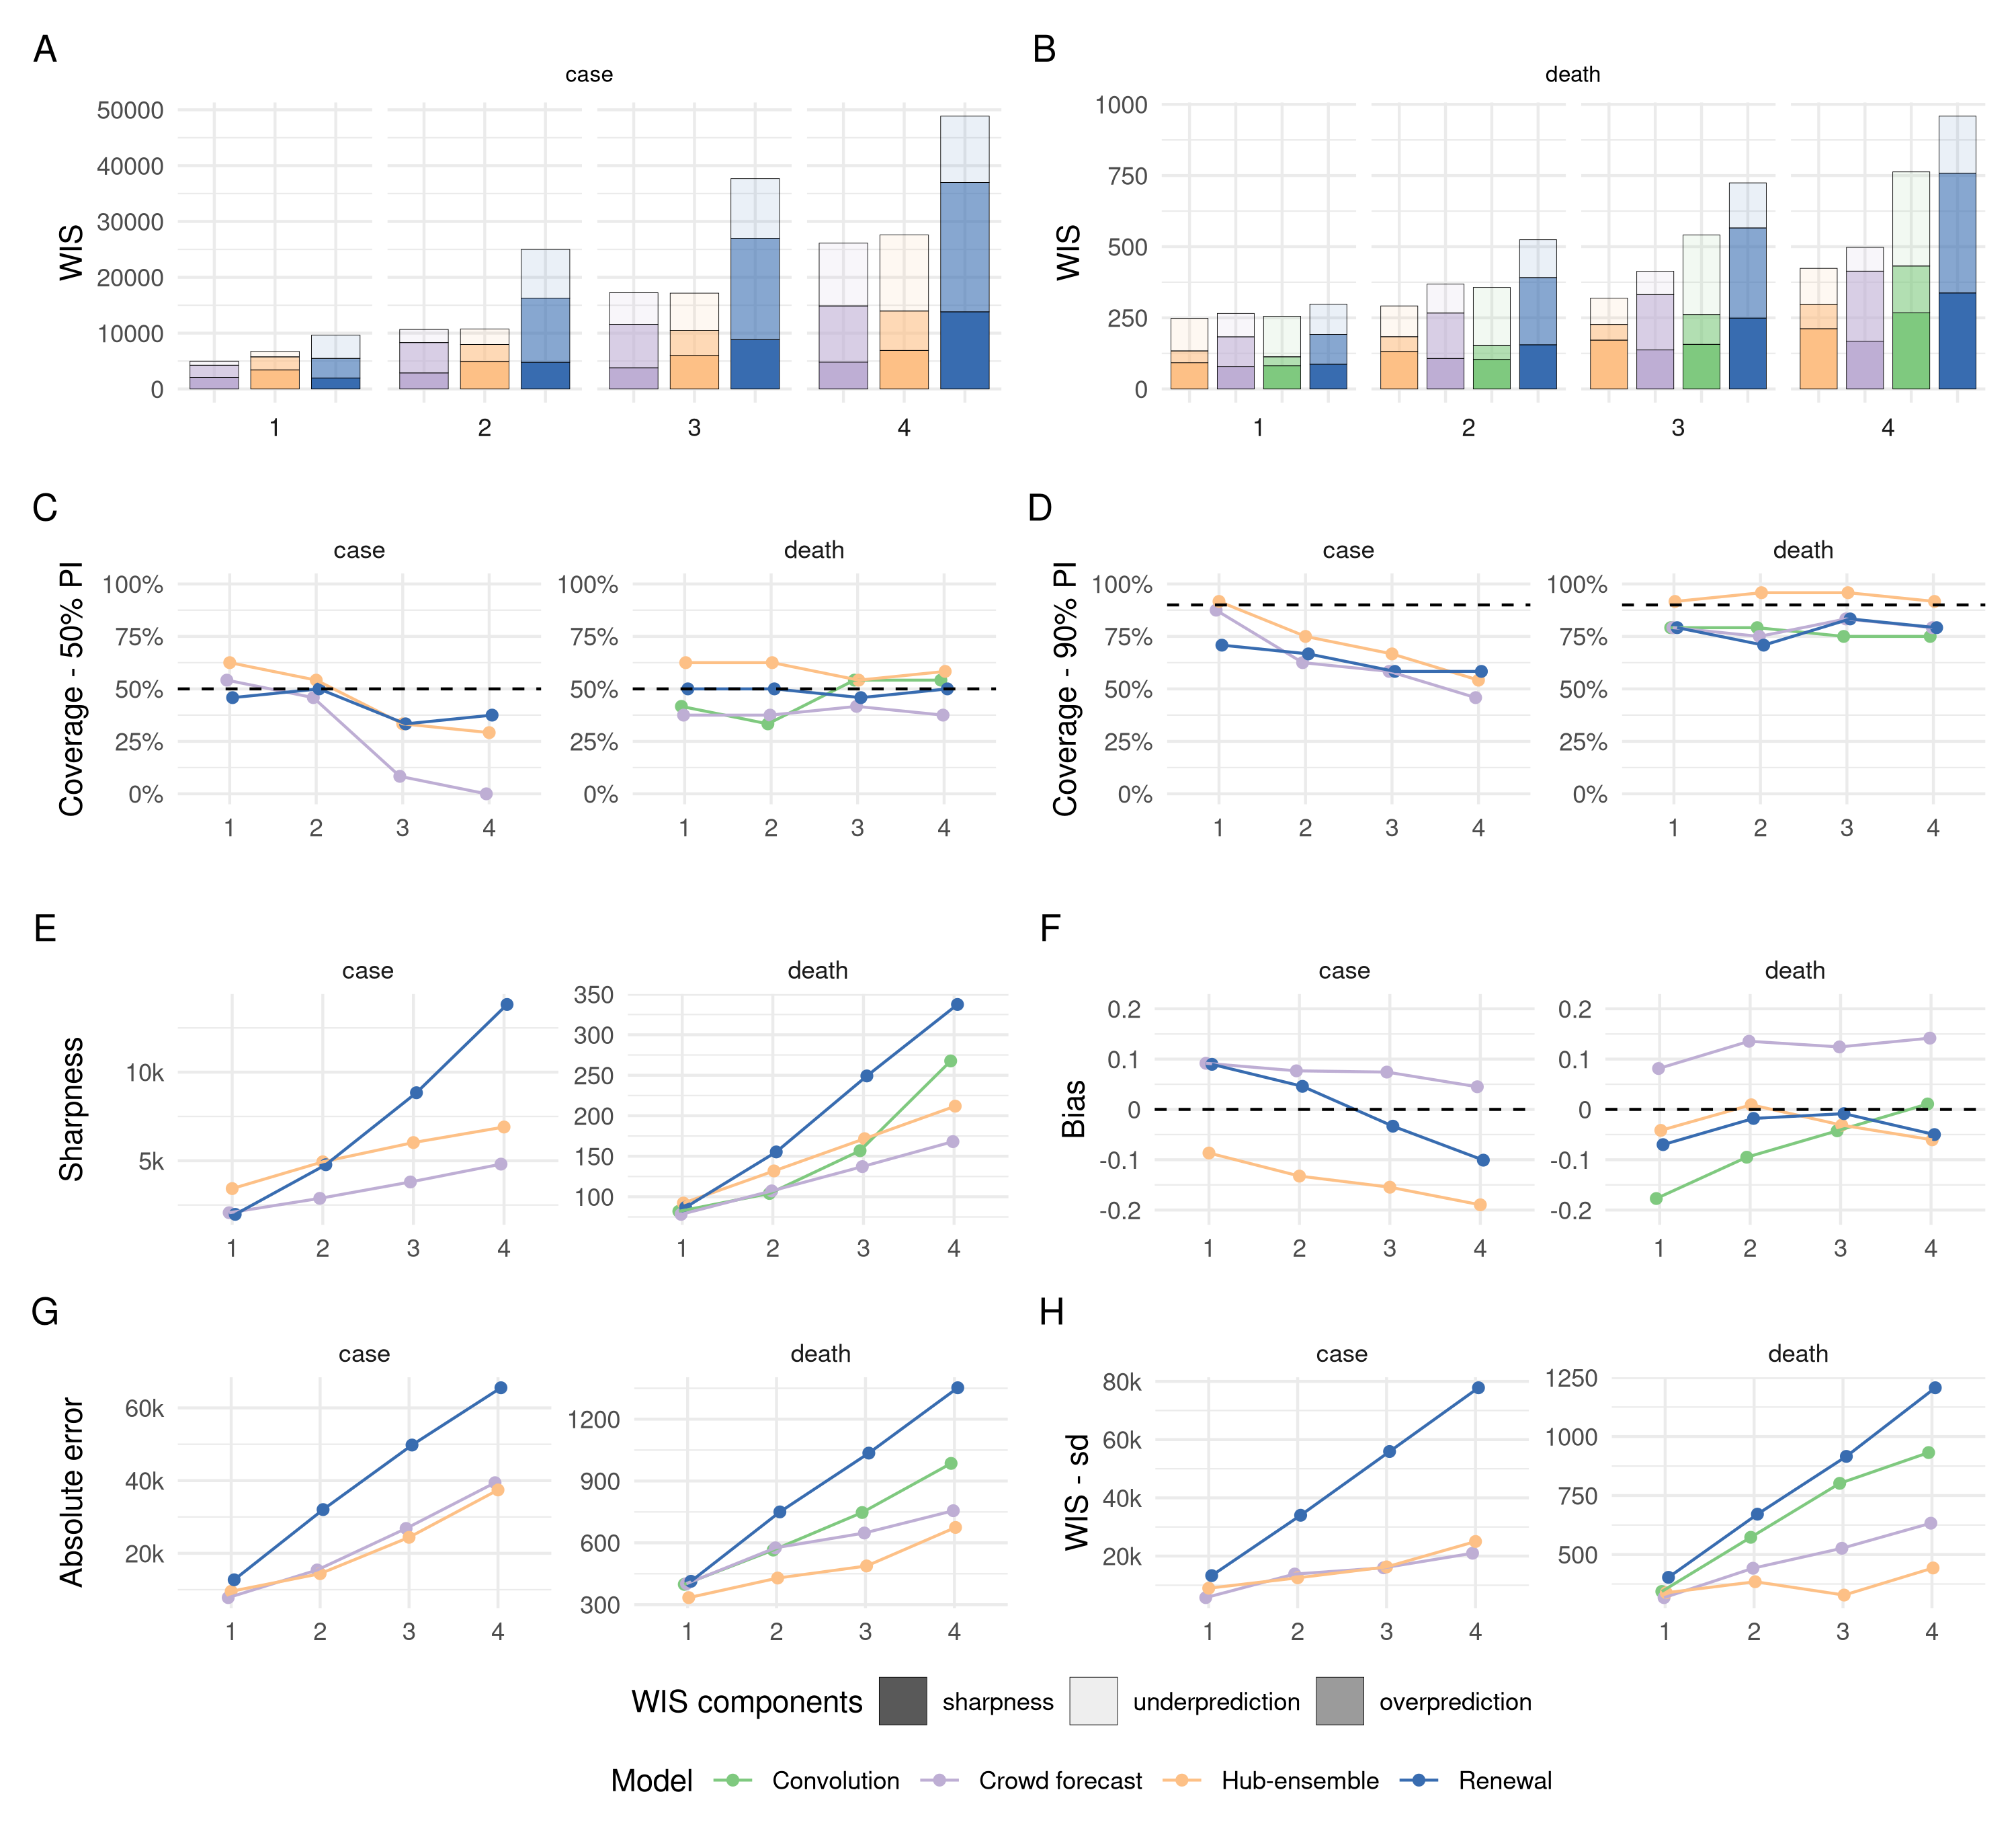
\includegraphics[width=1\linewidth,]{../../../analysis/plots/aggregate-performance-all-late-period-v4}
\caption{Visualisation of aggregate performance metrics across forecast horizons only for the period from December 14th 2020 on where all models were available. A, B: mean weighted interval score (WIS, lower indicates better performance) across horizons. WIS is decomposed into its components dispersion, over-prediction and under-prediction. C: Empirical coverage of the 50\% prediction intervals (50\% coverage is perfect). D: Empirical coverage of the 90\% prediction intervals. E: Dispersion (same as in panel A, B). Higher values mean greater dispersion of the forecast and imply ceteris paribus a worse score. F: Bias, i.e. general (relative) tendency to over- or underpredict. Values are between -1 (complete under-prediction) and 1 (complete over-prediction) and 0 ideally. G: Absolute error of the median forecast (lower is better). H. Standard deviation of all WIS values for different horizons}\label{fig:agg-performance-all-late}
\end{figure}

\begin{table}[!h]
\caption{\label{tab:score-table-late-2}Scores for one and two week ahead forecasts (cut to three significant digits and rounded) calculated on forecasts made between December 14th 2020 and March 1st 2021. Numbers in brackets show the metrics relative to the Hub ensemble (i.e. the median ensemble of all other models submitted to the German and Polish Forecast Hub, excluding our contributions). WIS is the mean weighted interval score (lower values are better), WIS - sd is the standard deviation of all scores achieved by a model. Dispersion, over-prediction and under-prediction together sum up to the weighted interval score. Bias (between -1 and 1, 0 is ideal) represents the general average tendency of a model to over- or underpredict. 50\% and 90\%-coverage are the percentage of observed values that fell within the 50\% and 90\% prediction intervals of a model.\\\hspace{\textwidth}}

\centering
\resizebox{\linewidth}{!}{
\begin{tabular}{>{}llccccccccc}
\toprule
  & Model & WIS & WIS - sd & dispersion & Underpred. & Overpred. & Bias & Abs. error & 50\%-Cov. & 90\%-Cov.\\
\midrule
\addlinespace[0.3em]
\multicolumn{11}{l}{\textbf{Cases}}\\
\hline
\cellcolor{white}{} & Crowd forecast & 4980 (0.74) & 5730 (0.64) & 2070 (0.6) & 728 (0.74) & 2190 (0.94) & 0.09 & 7810 (0.82) & 0.54 & 0.88\\
\cmidrule{2-11}
\cellcolor{white}{} & Hub-ensemble & 6730 (1) & 8960 (1) & 3430 (1) & 978 (1) & 2330 (1) & -0.09 & 9550 (1) & 0.62 & 0.92\\
\cmidrule{2-11}
\cellcolor{white}{\multirow{-3}{*}{\raggedright\arraybackslash 1 wk ahead}} & Renewal & 9640 (1.43) & 13300 (1.48) & 1970 (0.57) & 4170 (4.26) & 3500 (1.5) & 0.09 & 12700 (1.33) & 0.46 & 0.71\\
\cmidrule{1-11}
\cellcolor{white}{} & Crowd forecast & 10700 (0.99) & 13800 (1.1) & 2880 (0.58) & 2350 (0.85) & 5430 (1.79) & 0.08 & 15400 (1.07) & 0.46 & 0.62\\
\cmidrule{2-11}
\cellcolor{white}{} & Hub-ensemble & 10800 (1) & 12500 (1) & 4940 (1) & 2780 (1) & 3030 (1) & -0.13 & 14400 (1) & 0.54 & 0.75\\
\cmidrule{2-11}
\cellcolor{white}{\multirow{-3}{*}{\raggedright\arraybackslash 2 wk ahead}} & Renewal & 25000 (2.31) & 34000 (2.72) & 4780 (0.97) & 8710 (3.13) & 11500 (3.8) & 0.05 & 32000 (2.22) & 0.50 & 0.67\\
\cmidrule{1-11}
\addlinespace[0.3em]
\multicolumn{11}{l}{\textbf{Deaths}}\\
\hline
\cellcolor{white}{} & Convolution & 255 (1.03) & 343 (1.01) & 82 (0.89) & 142 (1.23) & 31.1 (0.75) & -0.18 & 399 (1.19) & 0.42 & 0.79\\
\cmidrule{2-11}
\cellcolor{white}{} & Crowd forecast & 265 (1.07) & 317 (0.94) & 78.2 (0.85) & 82 (0.71) & 105 (2.52) & 0.08 & 402 (1.2) & 0.38 & 0.79\\
\cmidrule{2-11}
\cellcolor{white}{} & Hub-ensemble & 248 (1) & 338 (1) & 92.2 (1) & 115 (1) & 41.6 (1) & -0.04 & 334 (1) & 0.62 & 0.92\\
\cmidrule{2-11}
\cellcolor{white}{\multirow{-4}{*}{\raggedright\arraybackslash 1 wk ahead}} & Renewal & 298 (1.2) & 403 (1.19) & 87 (0.94) & 107 (0.93) & 105 (2.52) & -0.07 & 413 (1.24) & 0.50 & 0.79\\
\cmidrule{1-11}
\cellcolor{white}{} & Convolution & 357 (1.22) & 573 (1.49) & 104 (0.79) & 204 (1.89) & 48.8 (0.94) & -0.10 & 565 (1.32) & 0.33 & 0.79\\
\cmidrule{2-11}
\cellcolor{white}{} & Crowd forecast & 368 (1.26) & 442 (1.15) & 107 (0.81) & 102 (0.94) & 160 (3.08) & 0.14 & 576 (1.34) & 0.38 & 0.75\\
\cmidrule{2-11}
\cellcolor{white}{} & Hub-ensemble & 292 (1) & 385 (1) & 132 (1) & 108 (1) & 51.9 (1) & 0.01 & 429 (1) & 0.62 & 0.96\\
\cmidrule{2-11}
\cellcolor{white}{\multirow{-4}{*}{\raggedright\arraybackslash 2 wk ahead}} & Renewal & 524 (1.79) & 671 (1.74) & 155 (1.17) & 133 (1.23) & 236 (4.55) & -0.02 & 750 (1.75) & 0.50 & 0.71\\
\bottomrule
\end{tabular}}
\end{table}

\begin{table}[!h]
\caption{\label{tab:score-table-late-4}Scores for three and four week ahead forecasts (cut to three significant digits and rounded) calculated on forecasts made between December 14th 2020 and March 1st 2021. Numbers in brackets show the metrics relative to the Hub ensemble (i.e. the median ensemble of all other models submitted to the German and Polish Forecast Hub, excluding our contributions). WIS is the mean weighted interval score (lower values are better), WIS - sd is the standard deviation of all scores achieved by a model. Dispersion, over-prediction and under-prediction together sum up to the weighted interval score. Bias (between -1 and 1, 0 is ideal) represents the general average tendency of a model to over- or underpredict. 50\% and 90\%-coverage are the percentage of observed values that fell within the 50\% and 90\% prediction intervals of a model.\\\hspace{\textwidth}}

\centering
\resizebox{\linewidth}{!}{
\begin{tabular}{>{}llccccccccc}
\toprule
  & Model & WIS & WIS - sd & dispersion & Underpred. & Overpred. & Bias & Abs. error & 50\%-Cov. & 90\%-Cov.\\
\midrule
\addlinespace[0.3em]
\multicolumn{11}{l}{\textbf{Cases}}\\
\hline
\cellcolor{white}{} & Crowd forecast & 17200 (1) & 16000 (0.98) & 3800 (0.63) & 5660 (0.85) & 7770 (1.74) & 0.07 & 26800 (1.1) & 0.08 & 0.58\\
\cmidrule{2-11}
\cellcolor{white}{} & Hub-ensemble & 17200 (1) & 16300 (1) & 6030 (1) & 6670 (1) & 4470 (1) & -0.16 & 24400 (1) & 0.33 & 0.67\\
\cmidrule{2-11}
\cellcolor{white}{\multirow{-3}{*}{\raggedright\arraybackslash 3 wk ahead}} & Renewal & 37700 (2.19) & 55900 (3.43) & 8840 (1.47) & 10700 (1.6) & 18100 (4.05) & -0.03 & 49800 (2.04) & 0.33 & 0.58\\
\cmidrule{1-11}
\cellcolor{white}{} & Crowd forecast & 26100 (0.95) & 21000 (0.84) & 4810 (0.7) & 11300 (0.83) & 10100 (1.43) & 0.04 & 39400 (1.05) & 0.00 & 0.46\\
\cmidrule{2-11}
\cellcolor{white}{} & Hub-ensemble & 27600 (1) & 25000 (1) & 6900 (1) & 13600 (1) & 7060 (1) & -0.19 & 37400 (1) & 0.29 & 0.54\\
\cmidrule{2-11}
\cellcolor{white}{\multirow{-3}{*}{\raggedright\arraybackslash 4 wk ahead}} & Renewal & 48900 (1.77) & 77800 (3.11) & 13800 (2) & 11900 (0.88) & 23200 (3.29) & -0.10 & 65500 (1.75) & 0.38 & 0.58\\
\cmidrule{1-11}
\addlinespace[0.3em]
\multicolumn{11}{l}{\textbf{Deaths}}\\
\hline
\cellcolor{white}{} & Convolution & 541 (1.7) & 802 (2.45) & 157 (0.91) & 279 (3.01) & 105 (1.91) & -0.04 & 747 (1.53) & 0.54 & 0.75\\
\cmidrule{2-11}
\cellcolor{white}{} & Crowd forecast & 414 (1.3) & 526 (1.6) & 137 (0.8) & 82 (0.88) & 194 (3.52) & 0.12 & 648 (1.33) & 0.42 & 0.83\\
\cmidrule{2-11}
\cellcolor{white}{} & Hub-ensemble & 319 (1) & 328 (1) & 172 (1) & 92.7 (1) & 55.1 (1) & -0.03 & 488 (1) & 0.54 & 0.96\\
\cmidrule{2-11}
\cellcolor{white}{\multirow{-4}{*}{\raggedright\arraybackslash 3 wk ahead}} & Renewal & 724 (2.27) & 916 (2.79) & 249 (1.45) & 158 (1.7) & 317 (5.75) & -0.01 & 1040 (2.13) & 0.46 & 0.83\\
\cmidrule{1-11}
\cellcolor{white}{} & Convolution & 763 (1.8) & 932 (2.1) & 268 (1.26) & 331 (2.63) & 164 (1.91) & 0.01 & 985 (1.46) & 0.54 & 0.75\\
\cmidrule{2-11}
\cellcolor{white}{} & Crowd forecast & 498 (1.17) & 633 (1.43) & 168 (0.79) & 83.6 (0.66) & 246 (2.87) & 0.14 & 756 (1.12) & 0.38 & 0.79\\
\cmidrule{2-11}
\cellcolor{white}{} & Hub-ensemble & 424 (1) & 443 (1) & 212 (1) & 126 (1) & 85.7 (1) & -0.06 & 675 (1) & 0.58 & 0.92\\
\cmidrule{2-11}
\cellcolor{white}{\multirow{-4}{*}{\raggedright\arraybackslash 4 wk ahead}} & Renewal & 959 (2.26) & 1210 (2.73) & 337 (1.59) & 200 (1.59) & 421 (4.91) & -0.05 & 1350 (2) & 0.50 & 0.79\\
\bottomrule
\end{tabular}}
\end{table}

\clearpage

\hypertarget{overview-of-models-and-forecasters}{%
\subsection{Overview of models and
forecasters}\label{overview-of-models-and-forecasters}}

\begin{longtable}[t]{>{\raggedright\arraybackslash}p{4.5cm}>{\raggedright\arraybackslash}p{7.3cm}}
\caption{\label{tab:table-ensemble-versions}Overview of the models and ensembles used.}\\
\toprule
Name & Explanation\\
\midrule
\endfirsthead
\caption[]{Overview of the models and ensembles used. \textit{(continued)}}\\
\toprule
Name & Explanation\\
\midrule
\endhead

\endfoot
\bottomrule
\endlastfoot
\cellcolor{gray!6}{Hub-ensemble-realised} & \cellcolor{gray!6}{Official Forecast Hub median ensemble. Created by the Forecast Hub officially under the name 'KITCOVIDhub-median\_ensemble' and used as the default ensemble. Included are our crowd forecasts as well as the renewal model (with one missed submission on December 28 2020, but not the convolution model which was deemed to similar to the renewal model.}\\
\addlinespace \addlinespace
Hub-ensemble-realised-mean & Official Forecast Hub mean ensemble. Created by the Forecast Hub officially under the name 'KITCOVIDhub-mean\_ensemble'.\\
\addlinespace \addlinespace
\cellcolor{gray!6}{ \vphantom{1}} & \cellcolor{gray!6}{}\\
\addlinespace \addlinespace
Hub-ensemble & Version of the official Hub median ensemble which excludes all our contributions.\\
\addlinespace \addlinespace
\cellcolor{gray!6}{Hub-ensemble-mean} & \cellcolor{gray!6}{Version of the official Hub mean ensemble which excludes all our contributions.}\\
\addlinespace \addlinespace
Hub-ensemble-with-renewal, 
    Hub-ensemble-with-renewal-mean & Versions of the official Hub ensembles which of our contributions includes only the Renewal model.\\
\addlinespace \addlinespace
Hub-ensemble-with-crowd, 
\cellcolor{gray!6}{    Hub-ensemble-with-crowd-mean} & \cellcolor{gray!6}{Versions of the official Hub ensembles which of our contributions includes only the Crowd forecast.}\\
\addlinespace \addlinespace
Hub-ensemble-with-convolution, 
    Hub-ensemble-with-convolution-mean & Versions of the official Hub ensembles which of our contributions includes only the Convolution model (which originally was never included in any official Hub ensemble).\\
\addlinespace \addlinespace
Hub-ensemble-with-all, 
\cellcolor{gray!6}{    Hub-ensemble-with-all-mean} & \cellcolor{gray!6}{Versions of the official Hub ensembles which includes all our contributions. For cases, this is identical to the official Hub ensembles, but for deaths the convolution model was added.}\\
\addlinespace \addlinespace
 & \\
\addlinespace \addlinespace
\cellcolor{gray!6}{Crowd forecast} & \cellcolor{gray!6}{Submitted to the Forecast Hub as 'epiforecasts-EpiExpert'}\\
\addlinespace \addlinespace
Renewal model & Submitted to the Forecast Hub as 'epiforecasts-EpiNow2'\\
\addlinespace \addlinespace
\cellcolor{gray!6}{Convolution model} & \cellcolor{gray!6}{Submitted to the Forecast Hub as 'epiforecasts-EpiNow2\_secondary'}\\*
\end{longtable}

\begin{figure}[H]
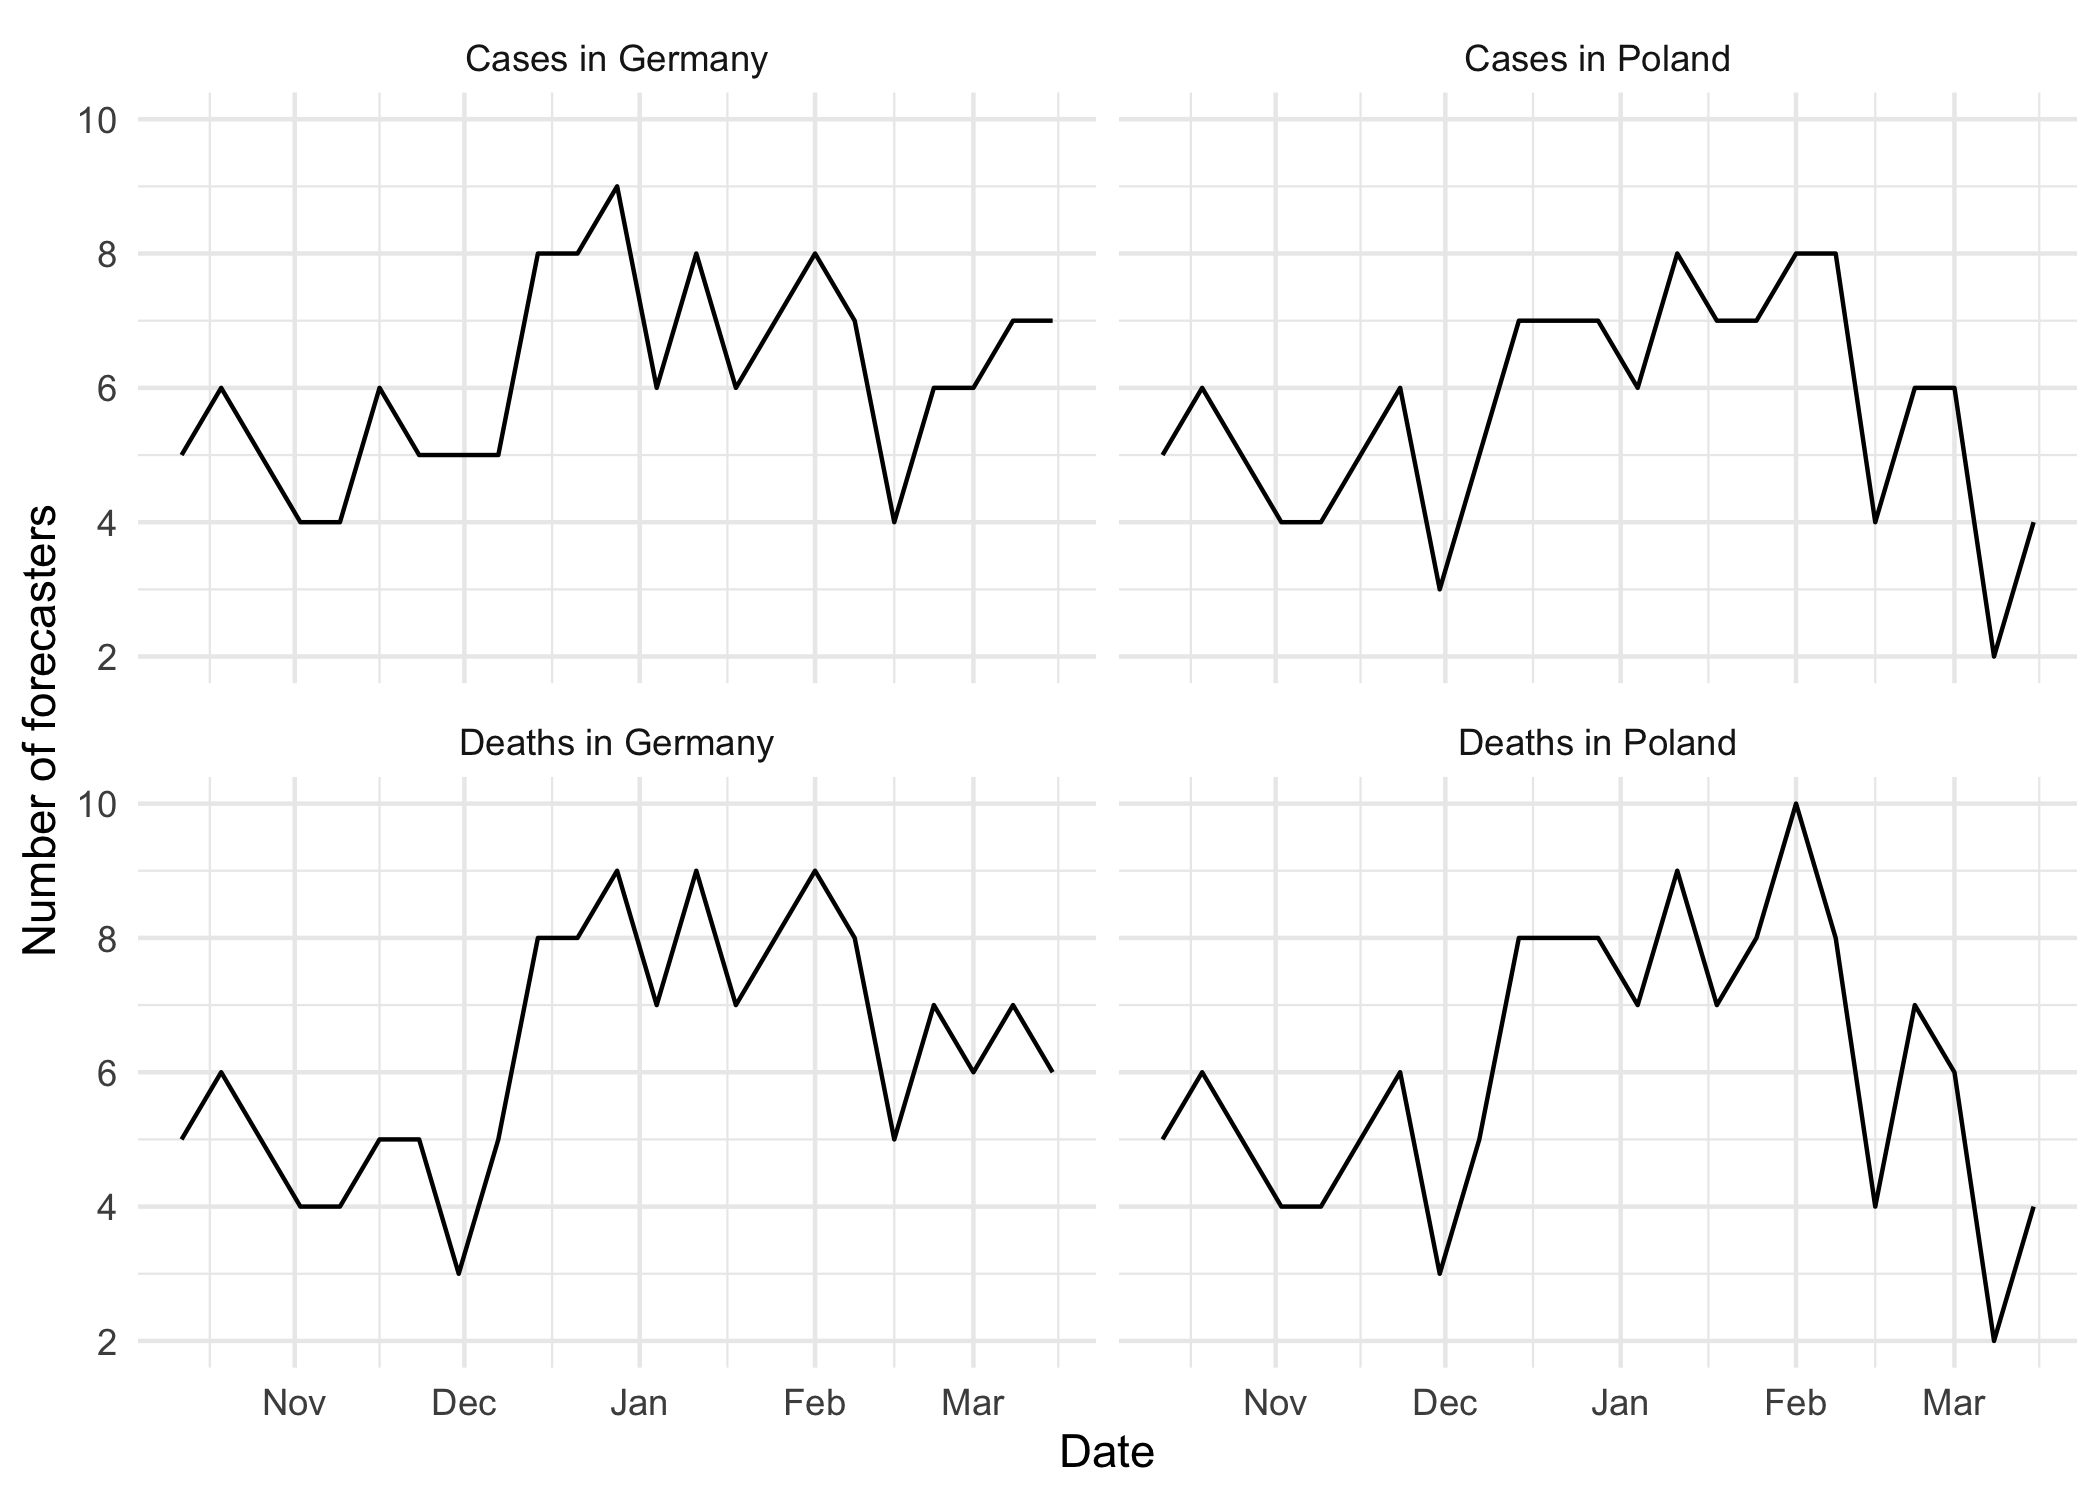
\includegraphics[width=1\linewidth,]{../../../analysis/plots/number-forecasters} 
\caption{Number of participants who submitted a forecast over time.}\label{fig:num-forecasters}
\end{figure}

\begin{figure}[H]
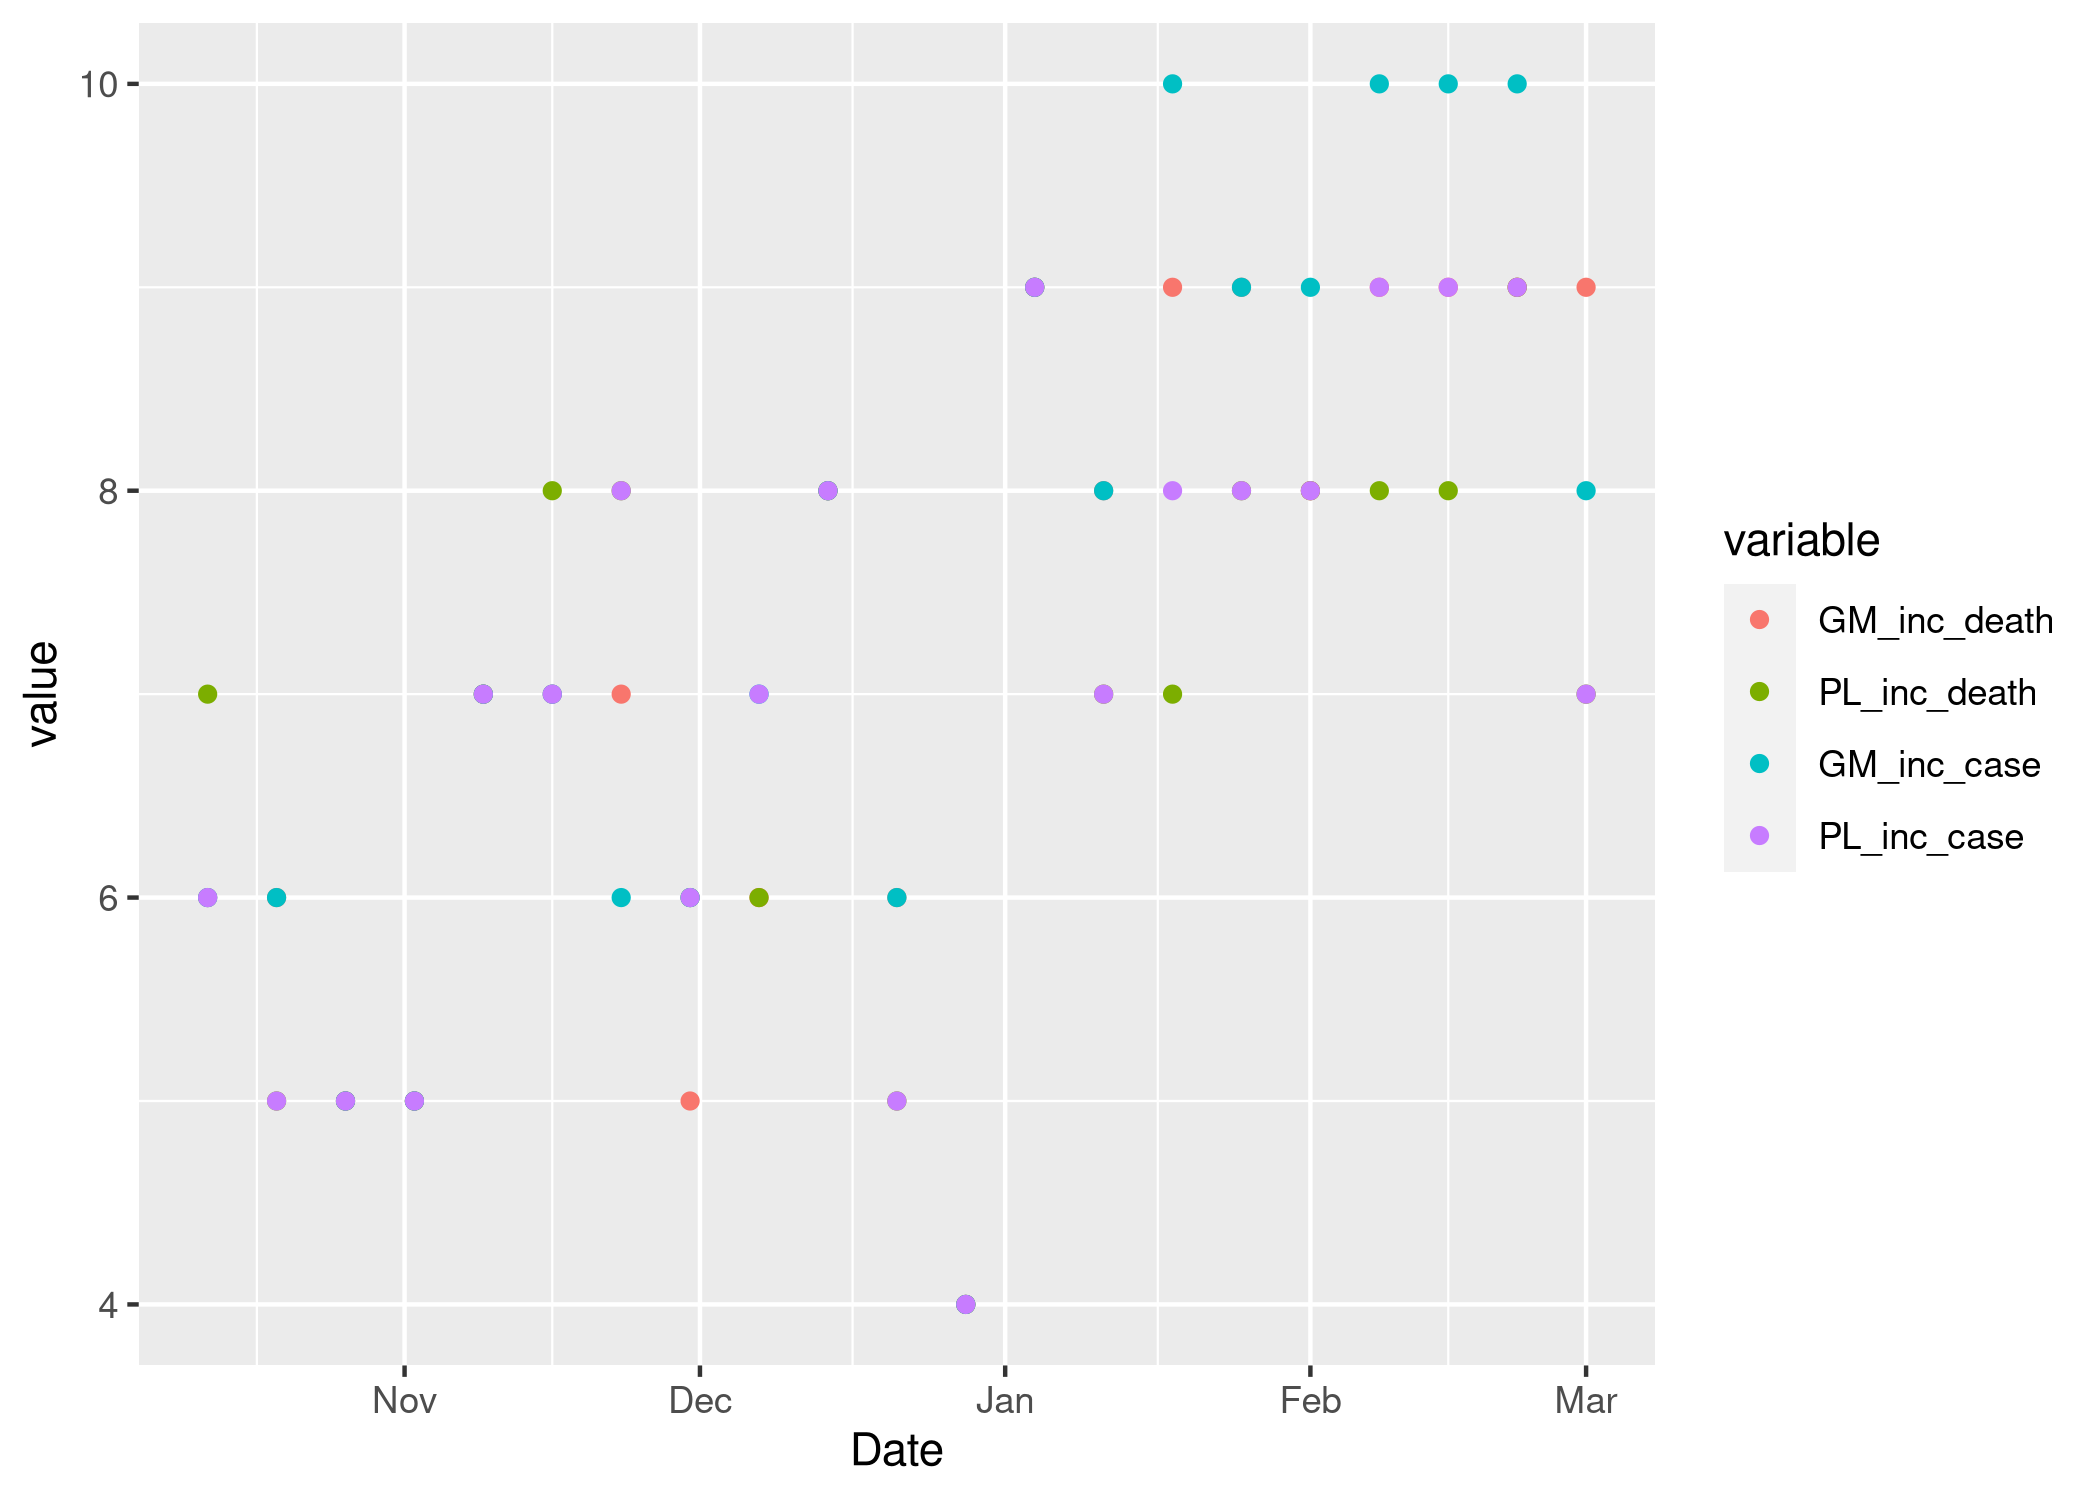
\includegraphics[width=1\linewidth,]{../../../analysis/plots/ensemble-members} 
\caption{Number of member models (including our crowd forecasts and the renewal model) in the official Hub ensemble. Note that the renewal model was not included in the ensemble on December 28th 2020.}\label{fig:num-ensemble-members}
\end{figure}

\clearpage

\hypertarget{comparison-of-crowd-forecasts-and-application-baseline}{%
\subsection{Comparison of crowd forecasts and application
baseline}\label{comparison-of-crowd-forecasts-and-application-baseline}}

\begin{figure}[H]
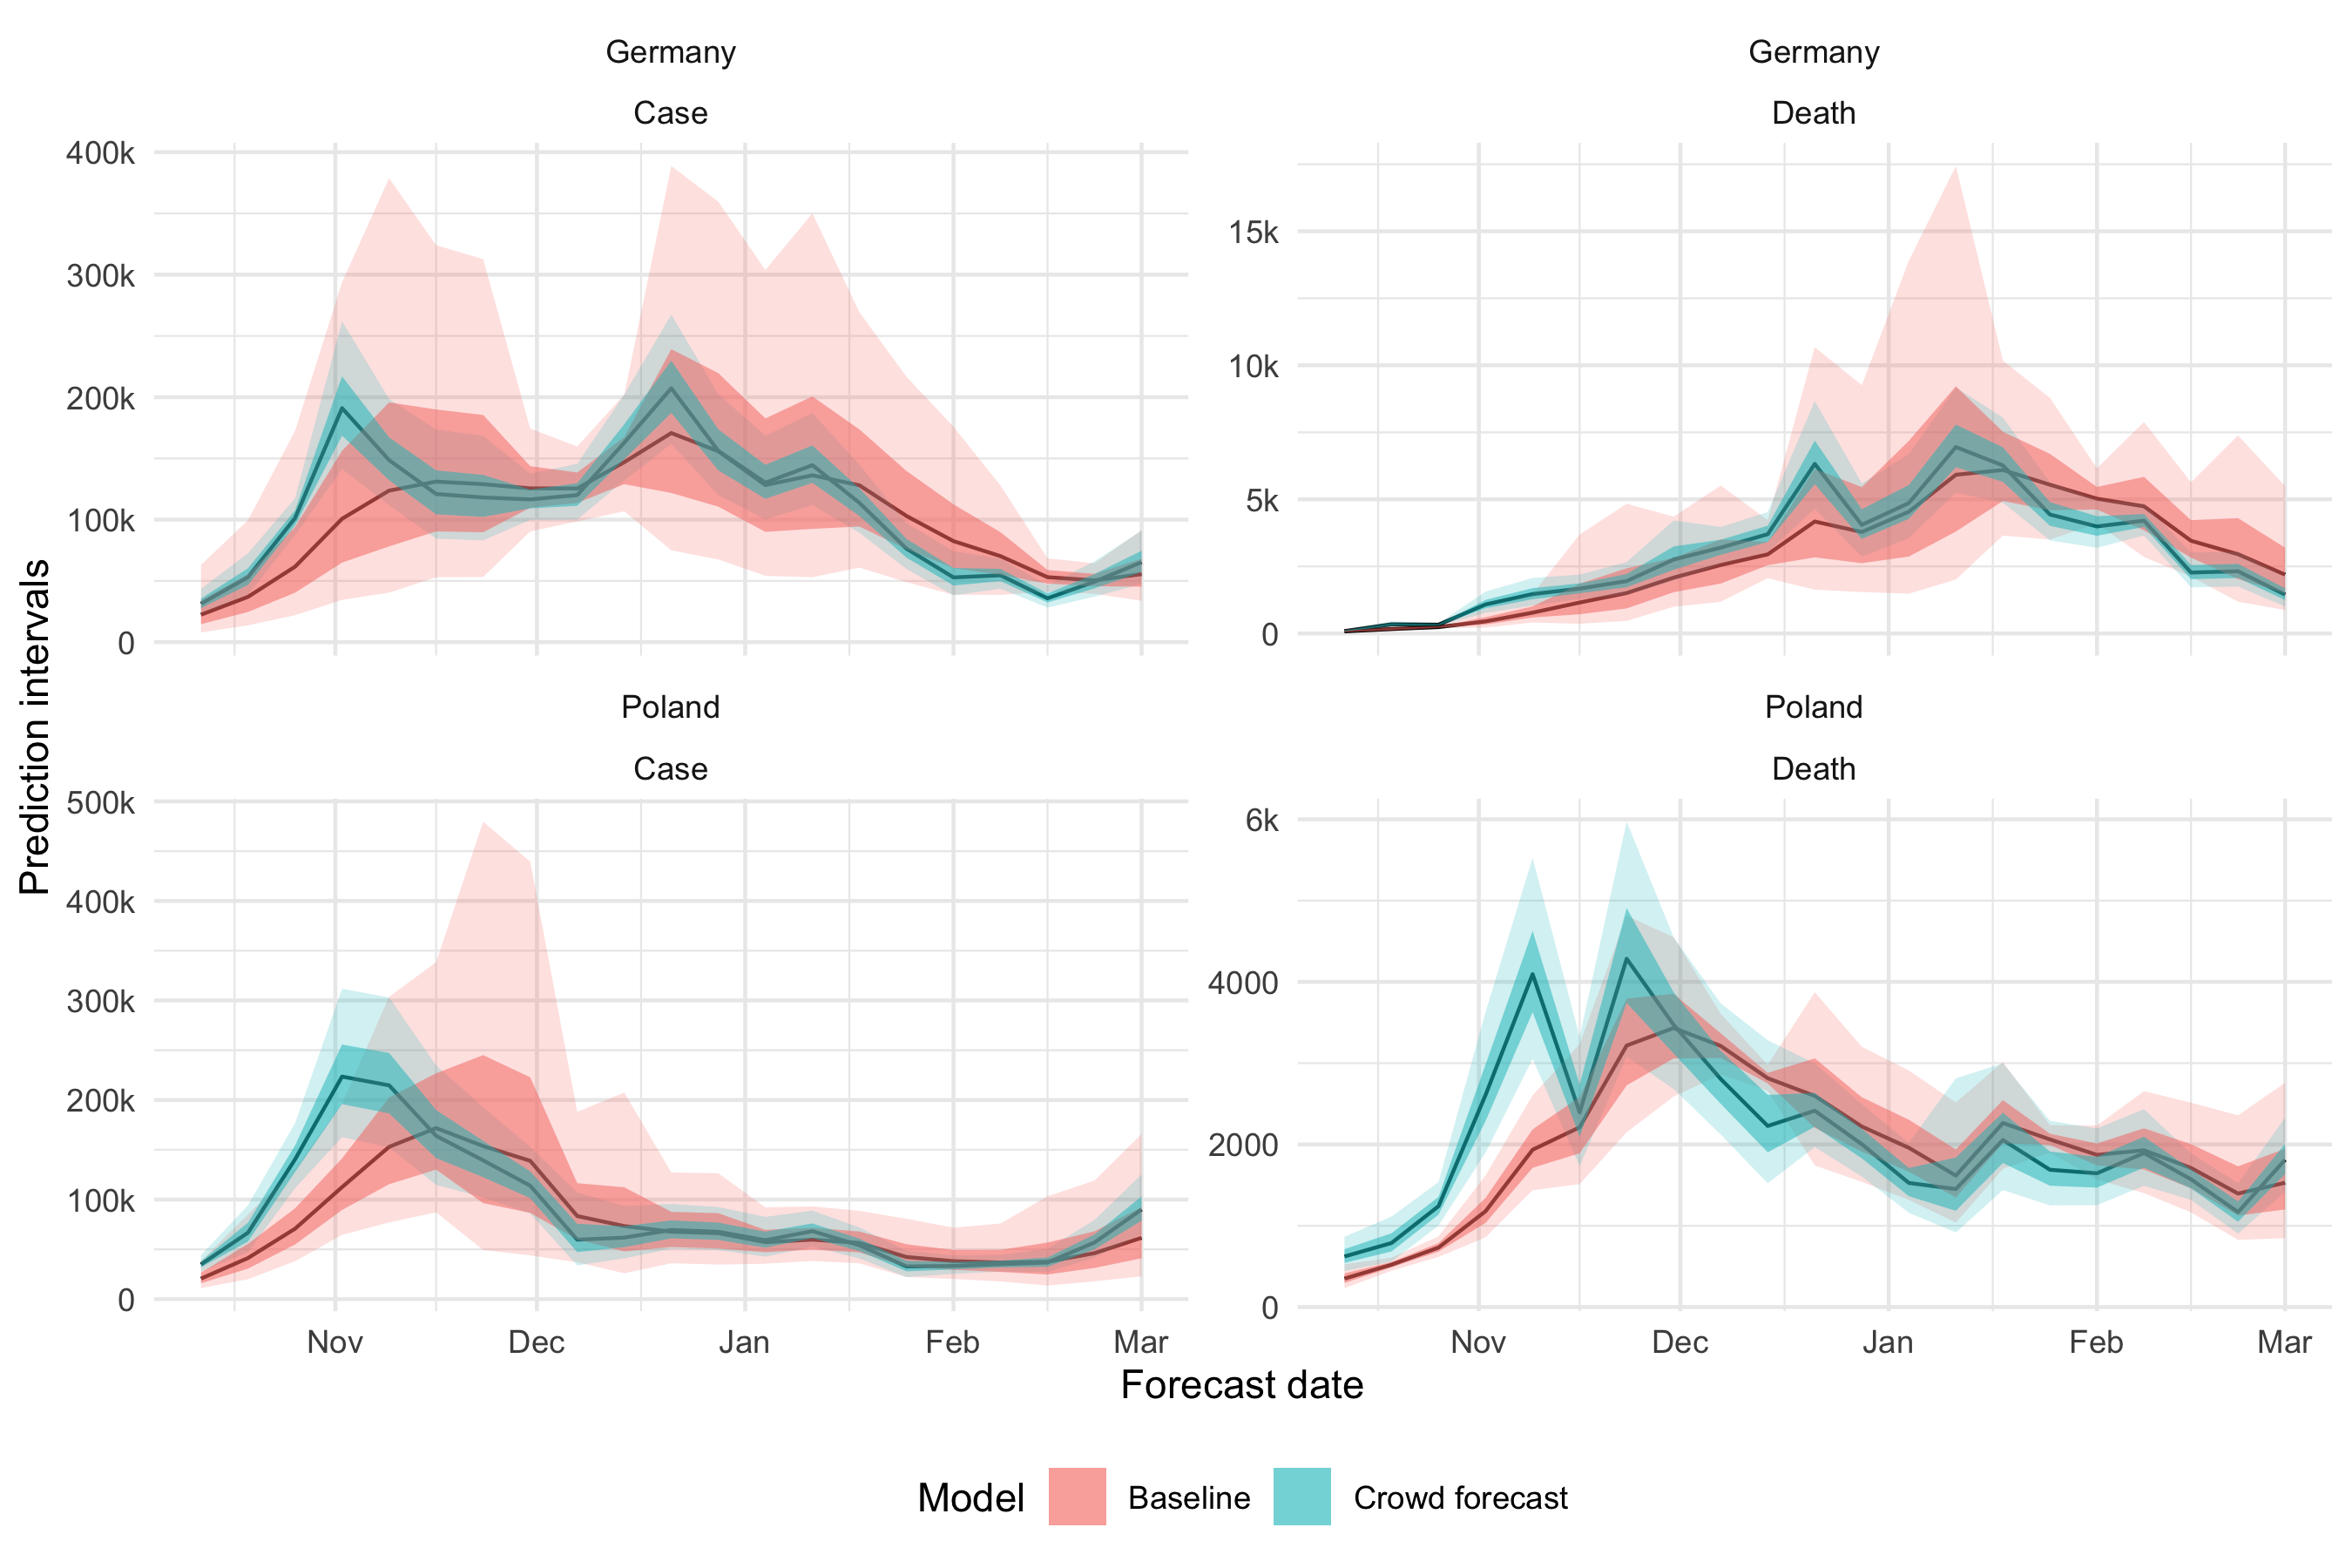
\includegraphics[width=1\linewidth,]{../../../analysis/plots/comparison-forecast-interals}
\caption{Crowd forecasts and baseline shown in the application for a two week horizon. Shown are the median, as well as the 50\% and 90\% prediction intervals (in order of decreasing opacity). For any given point in time, the baseline shown in red is what forecasters saw when they opened the app (the baseline shown was constant across all forecast horizons).}\label{fig:compare-forecasters}
\end{figure}


\end{document}
